\RequirePackage{luatex85}
\PassOptionsToPackage{unicode}{hyperref}
\PassOptionsToPackage{naturalnames}{hyperref}
\documentclass{article}
% \documentclass[english,aps,prd,onecolumn,showpacs,superscriptaddress,groupedaddress,fixfloats]{revtex4-1}
\usepackage{geometry}
\usepackage[cm]{fullpage}
\usepackage{parskip}
\usepackage{physics}
\usepackage{amsmath}
\usepackage{amssymb}
\usepackage[dvipsnames]{xcolor}
\usepackage[colorlinks,linkcolor=blue,citecolor=green]{hyperref}
\usepackage{array}
\usepackage{longtable}
\usepackage{multirow}
\usepackage{comment}
\usepackage{graphicx}
\usepackage{cite}
\usepackage{amsfonts}
\usepackage{bm}
\usepackage{slashed}
\usepackage{dsfont}
\usepackage{mathtools}
\usepackage[compat=1.1.0]{tikz-feynman}
\usepackage{tikz}
\usetikzlibrary{hobby}
\usepackage{pgfplots}
\pgfplotsset{compat=newest}
\usepackage{simpler-wick} 
\usepackage{mathrsfs}
\usepackage{xparse}
\usepackage{enumerate}
\usepackage{extarrows}
\usepackage[caption=false]{subfig}
% ==============================================================================
% Endnotes
% ==============================================================================
\usepackage{enotez}
% HOWTO: 
% \endnote{}
% Print the notes by adding the following to the end of the document: 
% \printendnotes

% ==============================================================================
% Minted
% ==============================================================================
\usepackage{minted}
\usemintedstyle{colorful}
% HOWTO: 
% \begin{minted}{lang}
% 	code
% \end{minted}{lang}

% ==============================================================================
% Changes: comments and highlights
% ==============================================================================
\let\comment\undefined
\usepackage[highlightmarkup=uwave]{changes}

\allowdisplaybreaks

% ==============================================================================
% mathtools
% ==============================================================================
\newcommand\MTkillspecial[1]{% helper macro
	\bgroup
	\catcode`\&=9
	\let\\\relax%
	\scantokens{#1}%
	\egroup
	}
\DeclarePairedDelimiter\BraceM\{\}
\reDeclarePairedDelimiterInnerWrapper\BraceM{star}{
	\mathopen{#1\vphantom{\MTkillspecial{#2}}\kern-\nulldelimiterspace\right.}
	#2
	\mathclose{\left.\kern-\nulldelimiterspace\vphantom{\MTkillspecial{#2}}#3}
	}
\DeclarePairedDelimiter\bracketM{[}{]}
\reDeclarePairedDelimiterInnerWrapper\bracketM{star}{
	\mathopen{#1\vphantom{\MTkillspecial{#2}}\kern-\nulldelimiterspace\right.}
	#2
	\mathclose{\left.\kern-\nulldelimiterspace\vphantom{\MTkillspecial{#2}}#3}
	}
\let\Bqty\relax
\let\bqty\relax
\newcommand{\Bqty}[1]{\BraceM*{#1}}
\newcommand{\bqty}[1]{\bracketM*{#1}}
\DeclarePairedDelimiter\ceil{\lceil}{\rceil}
\DeclarePairedDelimiter\floor{\lfloor}{\rfloor}

% ==============================================================================
% ifthen for User-definition
% ==============================================================================
\usepackage{ifthen}
% HOWTO:
% \ifthenelse{<test>}{<code for true>}{<code for false>}

% ==============================================================================
% User Definition
% ==============================================================================
\newcommand{\red}[1]{{\color{red}#1}}
\newcommand{\mm}[1]{\frac{\dd^4#1}{(2\pi)^4}}
\newcommand{\mme}[1]{\frac{\dd^3\vb{#1}}{(2\pi)^3}}
\newcommand{\mmd}[2][d]{\ifthenelse{\equal{#1}{1}}{\frac{\dd {#2}}{2\pi}}{\frac{\dd^{#1}{#2}}{(2\pi)^{#1}}}}

\newcommand{\glprog}[2]{\int\frac{\dd #1}{2\pi}\frac{ie^{-i#1 #2}}{#1+i\epsilon}}

\makeatletter
\newcommand{\pushright}[1]{\ifmeasuring@#1\else\omit\hfill$\displaystyle#1$\fi\ignorespaces}
\newcommand{\pushleft}[1]{\ifmeasuring@#1\else\omit$\displaystyle#1$\hfill\fi\ignorespaces}
\makeatother

\NewDocumentCommand\NL{s}{%
  \IfBooleanTF#1%
    {\notag\\\times}% If a star is seen
    {\notag\\}%     If no star is seen
}



% ==============================================================================
% Tikz-Feynman Externalization
% ==============================================================================
\usepackage{shellesc}
\usetikzlibrary{external}
\usepgfplotslibrary{external}
\tikzexternalize[shell escape=-enable-write18,prefix=./QuasiPDF2L/,system call={lualatex \tikzexternalcheckshellescape -halt-on-error -interaction=batchmode -jobname "\image" "\texsource"},up to date check=md5]

\tikzfeynmanset{
	Eikonal/.style={
		/tikz/draw=none,
		/tikz/decoration={name=none},
		/tikz/postaction={
			/tikz/draw,
			/tikz/double distance=2pt,
			% /tikzfeynman/with arrow=0.5,
		},
	},
	tikzmom/.code n args={4}{
		\def\tempa{#1}
		\def\tempb{#2}
		\def\tempc{#3}
		\def\tempd{#4}

		\ifx \empty\tempa 
			\pgfkeysalso{momentum/arrow shorten={0.15}} % default value
		\else \pgfkeysalso{momentum/arrow shorten={#1}}
		\fi

		\ifx \empty\tempb 
			\pgfkeysalso{momentum/arrow distance={3mm}} % default value
		\else \pgfkeysalso{momentum/arrow distance={#2}}
		\fi

		\ifx \empty\tempc 
			\pgfkeysalso{momentum/label distance={0pt}} % default value
		\else \pgfkeysalso{momentum/label distance={#3}}
		\fi

		\pgfkeysalso{momentum={#4}}
	},
	tikzmom'/.code n args={4}{
		\def\tempa{#1}
		\def\tempb{#2}
		\def\tempc{#3}
		\def\tempd{#4}

		\ifx \empty\tempa 
			\pgfkeysalso{momentum/arrow shorten={0.15}} % default value
		\else \pgfkeysalso{momentum/arrow shorten={#1}}
		\fi

		\ifx \empty\tempb 
			\pgfkeysalso{momentum/arrow distance={3mm}} % default value
		\else \pgfkeysalso{momentum/arrow distance={#2}}
		\fi

		\ifx \empty\tempc 
			\pgfkeysalso{momentum/label distance={0pt}} % default value
		\else \pgfkeysalso{momentum/label distance={#3}}
		\fi

		\pgfkeysalso{momentum'={#4}}
	},
	half right/.append style={
		/tikz/looseness=2
	},
	half left/.append style={
		/tikz/looseness=2
	}
}

% ==============================================================================
% Tikz-Feynman Auxiliary
% ==============================================================================
\def\FDWidth{3cm}
\def\FDHeight{3cm}
\def\FDWidthS{2cm}
\def\FDHeightS{2cm}


\makeatletter
\renewcommand\subparagraph{%
 \@startsection {subparagraph}{5}{1em }{1.25ex \@plus 1ex
 \@minus .2ex}{-1em}{\normalfont \normalsize \bfseries }}%
\makeatother

\newcommand{\ZR}[1]{\textcolor{LimeGreen}{#1}}
\newcommand{\CJ}[1]{\textcolor{RoyalBlue}{#1}}
\newcommand{\WN}[1]{\textcolor{RawSienna}{#1}}
\newcommand{\WNZF}{\WN{Zero FIRE.py input file. }}
\newcommand{\WNOF}{\WN{Numbers overflow. }}
\newcommand{\WNNH}{\WN{Not handled eqn. }}
\newcommand{\WNDIV}{\WN{Divergent integrand. }}
\newcommand{\WNGINAC}{\WN{Failed in GiNaC\_Parallel! }}
\newcommand{\WNDZ}{\WN{power::eval(): division by zero. }}

\title{Two Loop Matching for Quasi PDF}
\author{Yingsheng Huang}
\begin{document}
\maketitle
\tableofcontents

\clearpage

\section{Renormalization}
\subsection{One loop diagrams}
\begin{figure}[!htpb]
	\centering
	\hfil\subfloat[8]{
		\centering
		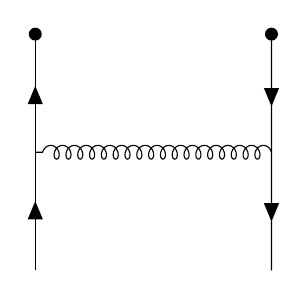
\begin{tikzpicture}[baseline=($(a)!0.5!(exa)$.base)]
			\begin{feynman}
				\node[dot] (a);
				\node[right=\FDWidth of a,dot] (b);open
				\vertex[below=\FDHeight of a] (exa);
				\vertex[below=\FDHeight of b] (exb);
				\vertex at ($(exa)!0.5!(a)$) (a1);
				\vertex at ($(exb)!0.5!(b)$) (b1);
				\diagram*{
				% (a) --[Eikonal] (b);
				(exa) --[fermion] (a1) --[fermion] (a);
				(b) --[fermion] (b1) --[fermion] (exb);
				(b1) --[gluon] (a1);
				};
			\end{feynman}
		\end{tikzpicture}
		\label{2:--}
	}\hfil
	\subfloat[4]{
		\centering
		\begin{tikzpicture}[baseline=($(a)!0.5!(exa)$.base)]
			\begin{feynman}
				\node[dot] (a);
				\node[right=\FDWidth of a,dot] (b);
				\vertex at ($(a)!0.5!(b)$) (o);
				\vertex[below=\FDHeight of a] (exa);
				\vertex[below=\FDHeight of b] (exb);
				\vertex at ($(exa)!0.5!(a)$) (a1);
				\vertex at ($(exb)!0.5!(b)$) (b1);
				\diagram*{
				(o) --[Eikonal] (b);
				(exa) --[fermion] (a1) --[fermion] (a);
				(b) --[fermion] (exb);
				(a1) --[gluon] (o);
				};
			\end{feynman}
		\end{tikzpicture}
		\label{2/-}
	}\hfil
	\subfloat[3]{
		\centering
		\begin{tikzpicture}[baseline=($(a)!0.5!(exa)$.base)]
			\begin{feynman}
				\node[dot] (a);
				\node[right=\FDWidth of a,dot] (b);
				\vertex at ($(a)!0.5!(b)$) (o);
				\vertex[below=\FDHeight of a] (exa);
				\vertex[below=\FDHeight of b] (exb);
				\vertex at ($(exa)!0.5!(a)$) (a1);
				\vertex at ($(exb)!0.5!(b)$) (b1);
				\diagram*{
				(a) --[Eikonal] (o);
				(exa) --[fermion] (a);
				(b) --[fermion] (b1) --[fermion] (exb);
				(b1) --[gluon] (o);
				};
			\end{feynman}
		\end{tikzpicture}
		\label{2-`}
	}\hfil
	\subfloat[5]{
		\centering
		\begin{tikzpicture}[baseline=($(a)!0.5!(exa)$.base)]
			\begin{feynman}
				\node[dot] (a);
				\node[right=\FDWidth of a,dot] (b);
				\vertex at ($(a)!0.3!(b)$) (o1);
				\vertex at ($(a)!0.7!(b)$) (o2);
				\vertex[below=\FDHeight of a] (exa);
				\vertex[below=\FDHeight of b] (exb);
				\diagram*{
				(a) --[Eikonal] (o1);
				(b) --[Eikonal] (o2);
				(exa) --[fermion] (a);
				(b) --[fermion] (exb);
				(o1) --[gluon, half right] (o2);
				};
			\end{feynman}
		\end{tikzpicture}
		\label{2-v-}
	}\hfil\\\hfil
	\subfloat[1]{
		\centering
		\begin{tikzpicture}[baseline=($(a)!0.5!(exa)$.base)]
			\begin{feynman}
				\node[dot] (a);
				\node[right=\FDWidth of a,dot] (b);
				\vertex at ($(a)!0.5!(b)$) (o);
				\vertex[below=\FDHeight of a] (exa);
				\vertex[below=\FDHeight of b] (exb);
				\vertex at ($(exa)!0.5!(a)$) (a1);
				\vertex at ($(exb)!0.5!(b)$) (b1);
				\diagram*{
				(o) --[Eikonal] (a);
				(exa) --[fermion] (a1) --[fermion] (a);
				(b) --[fermion] (exb);
				(a1) --[gluon] (o);
				};
			\end{feynman}
		\end{tikzpicture}
		\label{2-/}
	}\hfil
	\subfloat[7]{
		\centering
		\begin{tikzpicture}[baseline=($(a)!0.5!(exa)$.base)]
			\begin{feynman}
				\node[dot] (a);
				\node[right=\FDWidth of a,dot] (b);
				\vertex at ($(a)!0.5!(b)$) (o);
				\vertex[below=\FDHeight of a] (exa);
				\vertex[below=\FDHeight of b] (exb);
				\vertex at ($(exa)!0.5!(a)$) (a1);
				\vertex at ($(exb)!0.5!(b)$) (b1);
				\diagram*{
				(b) --[Eikonal] (o);
				(exa) --[fermion] (a);
				(b) --[fermion] (b1) --[fermion] (exb);
				(b1) --[gluon] (o);
				};
			\end{feynman}
		\end{tikzpicture}
		\label{2`-}
	}\hfil
	\subfloat[2]{
		\centering
		\begin{tikzpicture}[baseline=($(a)!0.5!(exa)$.base)]
			\begin{feynman}
				\node[dot] (a);
				\node[right=\FDWidth of a,dot] (b);
				\vertex at ($(a)!0.5!(b)$) (o);
				\vertex at ($(a)!0.2!(b)$) (o1);
				\vertex at ($(a)!0.8!(b)$) (o2);
				\vertex[below=\FDHeight of a] (exa);
				\vertex[below=\FDHeight of b] (exb);
				\diagram*{
				(a) --[Eikonal] (o);
				(exa) --[fermion] (a);
				(b) --[fermion] (exb);
				(o1) --[gluon, half right] (o);
				};
			\end{feynman}
		\end{tikzpicture}
		\label{2-o}
	}\hfil
	\subfloat[6]{
		\centering
		\begin{tikzpicture}[baseline=($(a)!0.5!(exa)$.base)]
			\begin{feynman}
				\node[dot] (a);
				\node[right=\FDWidth of a,dot] (b);
				\vertex at ($(a)!0.5!(b)$) (o);
				\vertex at ($(a)!0.2!(b)$) (o1);
				\vertex at ($(a)!0.8!(b)$) (o2);
				\vertex[below=\FDHeight of a] (exa);
				\vertex[below=\FDHeight of b] (exb);
				\diagram*{
				(b) --[Eikonal] (o);
				(exa) --[fermion] (a);
				(b) --[fermion] (exb);
				(o) --[gluon, half right] (o2);
				};
			\end{feynman}
		\end{tikzpicture}
		\label{2o-}
	}\hfil\\\hfil
	\subfloat[]{
		\centering
		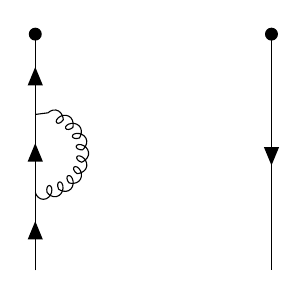
\begin{tikzpicture}[baseline=($(a)!0.5!(exa)$.base)]
			\begin{feynman}
				\node[dot] (a);
				\node[right=\FDWidth of a,dot] (b);
				\vertex[below=\FDHeight of a] (exa);
				\vertex[below=\FDHeight of b] (exb);
				\vertex at ($(exa)!0.33!(a)$) (a1);
				\vertex at ($(exa)!0.66!(a)$) (a2);
				\diagram*{
				% (a) --[Eikonal] (b);
				(exa) --[fermion] (a1) --[fermion] (a2) --[fermion] (a);
				(b) --[fermion] (exb);
				(a1) --[gluon, half right,looseness=2] (a2);
				};
			\end{feynman}
		\end{tikzpicture}
	}\hfil
	\subfloat[]{
		\centering
		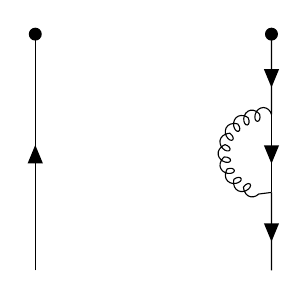
\begin{tikzpicture}[baseline=($(a)!0.5!(exa)$.base)]
			\begin{feynman}
				\node[dot] (a);
				\node[right=\FDWidth of a,dot] (b);
				\vertex[below=\FDHeight of a] (exa);
				\vertex[below=\FDHeight of b] (exb);
				\vertex at ($(exb)!0.33!(b)$) (b1);
				\vertex at ($(exb)!0.66!(b)$) (b2);
				\diagram*{
				% (a) --[Eikonal] (b);
				(exa) --[fermion] (a);
				(b) --[fermion] (b2) --[fermion] (b1) --[fermion] (exb);
				(b2) --[gluon, half right,looseness=2] (b1);
				};
			\end{feynman}
		\end{tikzpicture}
	}\hfil
	\caption{Diagrams of quasi PDF in Feynman gauge. }
\end{figure}
\subsection{Vertex corrections}
According to \cite{Ji:2015jwa}, the vertex correction diagrams in axial gauge (which corresponds to varieties of diagrams in general covariant gauge) don't have total UV divergence. Rather, they only have subdivergence for sub-diagrams. For example the first column (which involves Figure~3), second row of Table~1 in \cite{Ji:2015jwa} is composed of $\tilde q_{11}$ and $\tilde q_{12}$, thus we can find some representative diagrams and extract those components ($l\equiv l_1+l_2, \Delta l\equiv l_1-l_2$)
\begin{align}
	  & \begin{tikzpicture}[transform shape,scale=1,baseline=($(a)!0.5!(exa)$.base)]
		\begin{feynman}
			\node[dot] (a);
			\node[right=\FDWidth of a,dot] (b);
			\vertex at ($(a)!0.66!(b)$) (o);
			\vertex[below=\FDHeight of a] (exa);
			\vertex[below=\FDHeight of b] (exb);
			\vertex at ($(exa)!0.3!(a)$) (a1);
			\vertex at ($(exa)!0.7!(a)$) (a2);
			\vertex at ($(a1)!0.5!(a2)!1.2!-90:(a2)$) (g1);
			\vertex at ($(exb)!0.5!(b)$) (b1);
			\diagram*{
			(o) --[Eikonal,momentum=\(P-l_2\)] (b);
			(exa) --[fermion,momentum=\(P\)] (a1) --[fermion,momentum=\(l_1\)] (a2) --[fermion,momentum=\(l_2\)] (a);
			(a1) --[gluon,half right,looseness=2] (a2);
			(a1) --[quarter right,tikzmom'={0.2}{2mm}{-2pt}{$P-l_1$},draw=none] (g1) --[quarter right,tikzmom'={0.2}{2mm}{-2pt}{$\Delta l$},draw=none] (a2);
			(b) --[fermion,momentum=\(P\)] (exb);
			(g1) --[gluon,tikzmom'={0.2}{2mm}{-2pt}{$P-l_2$}] (o);
			};
		\end{feynman}
	\end{tikzpicture}\propto \int\mmd[d]{l_1}\mmd[d]{l_2}\frac{1}{\bqty{\slashed l_1-m}\bqty{\slashed l_2-m}\bqty{(P-l_1)^2}\bqty{(l_1-l_2)^2}\bqty{(P-l_2)^2}\bqty{n\cdot(P-l_2)}}
\end{align}
Take the $l_1\gg l_2$ limit, the integrand becomes
\begin{align}
	\frac{1}{\bqty{\slashed l_1-m}\bqty{(P-l_1)^2}\bqty{l_1^2}\bqty{\slashed l_2-m}\bqty{(P-l_2)^2}\bqty{n\cdot(P-l_2)}}
\end{align}
The integral involving $l_2$ is exactly the integral of $\tilde q_{12}$. By adding the gluon self-interacting vertex we can see that the sub-diagram is logarithmic divergent.

Take the $l_2\gg l_1$ limit, the integrand becomes
\begin{align}
	\frac{1}{\bqty{\slashed l_1-m}\bqty{(P-l_1)^2}\bqty{l_2^2}\bqty{\slashed l_2-m}\bqty{(P-l_2)^2}\bqty{n\cdot(P-l_2)}}
\end{align}

There's another limit where hard loop momentum flows through all paths except the one that's $\Delta l$ in our current diagram. This configuration gives a finite integral and a power-divergent integral which happens to be a scaleless integral as well. Thus this configuration won't contribute.

What we extracted above is only the $\tilde q_{12}$ part, now we will try on the $\tilde q_{11}$ part
\begin{align}
	  & \begin{tikzpicture}[transform shape,scale=1,baseline=($(a)!0.5!(exa)$.base)]
		\begin{feynman}
			\node[dot] (a);
			\node[right=\FDWidth of a,dot] (b);
			\vertex at ($(a)!0.66!(b)$) (o);
			\vertex[below=\FDHeight of a] (exa);
			\vertex[below=\FDHeight of b] (exb);
			\vertex at ($(exa)!0.25!(a)$) (a1);
			\vertex at ($(exa)!0.75!(a)$) (a2);
			\vertex at ($(exa)!0.5!(a)$) (am);
			\vertex at ($(exb)!0.5!(b)$) (bm);
			\diagram*{
			(exa) --[fermion,momentum=\(P\)] (a1) --[fermion,tikzmom'={0.3}{2mm}{-1pt}{$l_1$}] (am) --[fermion,tikzmom'={0.3}{2mm}{-1pt}{$l_1+l_2$}] (a2) --[fermion,momentum=\(P+l_2\)] (a);
			(a1) --[gluon,half left,looseness=2,tikzmom={0.3}{}{}{$P-l_1$}] (a2);
			(b) --[fermion,momentum=\(P+l_2\)] (bm)--[fermion,momentum=\(P\)] (exb);
			(bm) --[gluon,tikzmom={0.3}{}{}{$l_2$}] (am);
			};
		\end{feynman}
	\end{tikzpicture}\notag                                                                                                                                                                 \\
	  & \propto \int\mmd[d]{l_1}\mmd[d]{l_2}\frac{1}{\bqty{\slashed l_1-m}\bqty{\slashed l_1+\slashed l_2-m}\bqty{\slashed P+\slashed l_2-m}\bqty{\slashed P+\slashed l_2-m}\bqty{(P-l_1)^2}\bqty{l_2^2}}
\end{align}
In the $l_1\gg l_2$ limit we have
\begin{align}
	\frac{1}{\bqty{\slashed l_1-m}\bqty{\slashed l_1-m}\bqty{(P-l_1)^2}\bqty{\slashed P+\slashed l_2-m}\bqty{\slashed P+\slashed l_2-m}\bqty{l_2^2}}
\end{align}
and $\tilde q_{11}$ is factorized out.

Another example is the sixth row
\begin{align}
	\begin{tikzpicture}[transform shape,scale=1,baseline=($(a)!0.5!(exa)$.base)]
		\begin{feynman}
			\node[dot] (a);
			\node[right=\FDWidth of a,dot] (b);
			\vertex at ($(a)!0.5!(b)$) (o);
			\vertex at ($(a)!0.3!(b)$) (o1);
			\vertex at ($(a)!0.8!(b)$) (o2);
			\vertex[below=\FDHeight of a] (exa);
			\vertex[below=\FDHeight of b] (exb);
			\vertex at ($(exa)!0.4!(a)$) (a1);
			\diagram*{
			(o1) --[Eikonal] (o) --[Eikonal,tikzmom={0.2}{2mm}{-2pt}{$l_2$}] (o2) --[Eikonal] (b);
			(exa) --[fermion,momentum=\(P\)] (a1) --[fermion,momentum=\(l_1\)] (a);
			(b) --[fermion,momentum=\(P\)] (exb);
			(o) --[gluon, half right,tikzmom'={0.2}{2mm}{-2pt}{$P-l_1-l_2$}] (o2);
			(a1) --[gluon,tikzmom'={0.2}{2mm}{-2pt}{$P-l_1$}] (o1);
			};
		\end{feynman}
	\end{tikzpicture}\propto
	\int\mmd[d]{l_1}\mmd[d]{l_2}\frac{1}{\bqty{\slashed l_1-m}\bqty{(P-l_1)^2}\bqty{(P-l_1-l_2)^2}\bqty{n\cdot(P-l_1)}\bqty{n\cdot l_2}\bqty{n\cdot(P-l_1)}}
\end{align}
Take the $l_2\gg l_1$ limit, the integrand becomes
\begin{align}
	\frac{1}{\bqty{\slashed l_1-m}\bqty{(P-l_1)^2}\bqty{n\cdot(P-l_1)}\bqty{n\cdot(P-l_1)}\bqty{n\cdot l_2}\bqty{(P-l_2)^2}}
\end{align}
and the integral involving $l_2$ should give something proportional to $n\cdot (P-l_1)$, thus cancels one eikonal propagator, the remainder is the integral of $\tilde q_{12}$.

\subsection{Numerical results for one loop diagrams ($z=1/4$)}

\clearpage
\section{Real Diagrams}
\subsection{All diagrams}
Figure~\ref{re:sc} lists all self-conjugated real diagrams, and Figure~\ref{re:c} lists all non-self-conjugated diagrams, excluding their conjugates.
\renewcommand*\thesubfigure{\roman{subfigure}}
\begin{figure}[!hbtp]
	\centering\null\hfil
	\subfloat[10\red{/4.12}]{
		\begin{tikzpicture}[transform shape,scale=1,baseline=($(a)!0.5!(exa)$.base)]
			\begin{feynman}
				\node[dot] (a);
				\node[right=\FDWidth of a,dot] (b);
				\vertex[below=\FDHeight of a] (exa);
				\vertex[below=\FDHeight of b] (exb);
				% 
				\vertex at ($(a)!0.33!(b)$) (o13);
				\vertex at ($(a)!0.66!(b)$) (o23);
				\vertex at ($(a)!0.25!(b)$) (o14);
				\vertex at ($(a)!0.5!(b)$) (o12);
				\vertex at ($(a)!0.75!(b)$) (o34);
				% 
				\vertex at ($(a)!0.2!(b)$) (o15);
				\vertex at ($(a)!0.4!(b)$) (o25);
				\vertex at ($(a)!0.6!(b)$) (o35);
				\vertex at ($(a)!0.8!(b)$) (o45);
				% 
				\vertex at ($(o13)+1/4*(0,-\FDHeight)$) (o13m);
				\vertex at ($(o23)+1/4*(0,-\FDHeight)$) (o23m);
				% 
				\vertex at ($(exa)!0.25!(a)$) (a14);
				\vertex at ($(exa)!0.5!(a)$) (a12);
				\vertex at ($(exa)!0.75!(a)$) (a34);
				\vertex at ($(exa)!0.33!(a)$) (a13);
				\vertex at ($(exa)!0.66!(a)$) (a23);
				% 
				\vertex at ($(exb)!0.25!(b)$) (b14);
				\vertex at ($(exb)!0.5!(b)$) (b12);
				\vertex at ($(exb)!0.75!(b)$) (b34);
				\vertex at ($(exb)!0.33!(b)$) (b13);
				\vertex at ($(exb)!0.66!(b)$) (b23);
				% 
				\vertex at ($(a12)!0.33!(b12)$) (ab13);
				\vertex at ($(a12)!0.66!(b12)$) (ab23);
				\vertex at ($(a12)!0.5!(b12)$) (ab12);
				% 
				\vertex at ($(a14)!0.5!(a34)!1.2!-90:(a34)$) (g1);
				% 
				\diagram*{
				(a) --[Eikonal] (o13);
				(o23) --[Eikonal] (b);
				(exa) --[fermion] (a);
				(b) --[fermion] (exb);
				(o13) --[gluon] (o13m);
				(o23) --[gluon] (o23m);
				(o13m) --[gluon,half right,looseness=1.5] (o23m);
				(o13m) --[gluon] (o23m);
				};
			\end{feynman}
		\end{tikzpicture}
		\label{re:10}
	}\hfil
	\subfloat[11\red{/4.11}]{
		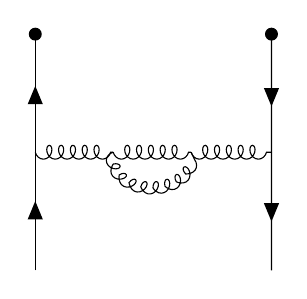
\begin{tikzpicture}[transform shape,scale=1,baseline=($(a)!0.5!(exa)$.base)]
			\begin{feynman}
				\node[dot] (a);
				\node[right=\FDWidth of a,dot] (b);
				\vertex[below=\FDHeight of a] (exa);
				\vertex[below=\FDHeight of b] (exb);
				% 
				\vertex at ($(a)!0.33!(b)$) (o13);
				\vertex at ($(a)!0.66!(b)$) (o23);
				\vertex at ($(a)!0.25!(b)$) (o14);
				\vertex at ($(a)!0.5!(b)$) (o12);
				\vertex at ($(a)!0.75!(b)$) (o34);
				% 
				\vertex at ($(a)!0.2!(b)$) (o15);
				\vertex at ($(a)!0.4!(b)$) (o25);
				\vertex at ($(a)!0.6!(b)$) (o35);
				\vertex at ($(a)!0.8!(b)$) (o45);
				% HOWTO: One can modify this to get vertexes lower than the gauge link line. 
				\vertex at ($(o13)+1/4*(0,-\FDHeight)$) (o13m);
				\vertex at ($(o23)+1/4*(0,-\FDHeight)$) (o23m);
				% 
				\vertex at ($(exa)!0.25!(a)$) (a14);
				\vertex at ($(exa)!0.5!(a)$) (a12);
				\vertex at ($(exa)!0.75!(a)$) (a34);
				\vertex at ($(exa)!0.33!(a)$) (a13);
				\vertex at ($(exa)!0.66!(a)$) (a23);
				% 
				\vertex at ($(exb)!0.25!(b)$) (b14);
				\vertex at ($(exb)!0.5!(b)$) (b12);
				\vertex at ($(exb)!0.75!(b)$) (b34);
				\vertex at ($(exb)!0.33!(b)$) (b13);
				\vertex at ($(exb)!0.66!(b)$) (b23);
				% 
				\vertex at ($(a12)!0.33!(b12)$) (ab13);
				\vertex at ($(a12)!0.66!(b12)$) (ab23);
				\vertex at ($(a12)!0.5!(b12)$) (ab12);
				% 
				\vertex at ($(a14)!0.5!(a34)!1.2!-90:(a34)$) (g1);
				% 
				\diagram*{
				(exa) --[fermion] (a12) --[fermion] (a);
				(b) --[fermion] (b12) --[fermion] (exb);
				(a12) --[gluon] (ab13) --[gluon] (ab23) --[gluon] (b12);
				(ab13) --[gluon,half right] (ab23);
				};
			\end{feynman}
		\end{tikzpicture}
		\label{}
	}\hfil
	\subfloat[26\red{/4.12}]{
		\begin{tikzpicture}[transform shape,scale=1,baseline=($(a)!0.5!(exa)$.base)]
			\begin{feynman}
				\node[dot] (a);
				\node[right=\FDWidth of a,dot] (b);
				\vertex[below=\FDHeight of a] (exa);
				\vertex[below=\FDHeight of b] (exb);
				% 
				\vertex at ($(a)!0.33!(b)$) (o13);
				\vertex at ($(a)!0.66!(b)$) (o23);
				\vertex at ($(a)!0.25!(b)$) (o14);
				\vertex at ($(a)!0.5!(b)$) (o12);
				\vertex at ($(a)!0.75!(b)$) (o34);
				% 
				\vertex at ($(a)!0.2!(b)$) (o15);
				\vertex at ($(a)!0.4!(b)$) (o25);
				\vertex at ($(a)!0.6!(b)$) (o35);
				\vertex at ($(a)!0.8!(b)$) (o45);
				% 
				\vertex at ($(o13)+1/4*(0,-\FDHeight)$) (o13m);
				\vertex at ($(o23)+1/4*(0,-\FDHeight)$) (o23m);
				% 
				\vertex at ($(exa)!0.25!(a)$) (a14);
				\vertex at ($(exa)!0.5!(a)$) (a12);
				\vertex at ($(exa)!0.75!(a)$) (a34);
				\vertex at ($(exa)!0.33!(a)$) (a13);
				\vertex at ($(exa)!0.66!(a)$) (a23);
				% 
				\vertex at ($(exb)!0.25!(b)$) (b14);
				\vertex at ($(exb)!0.5!(b)$) (b12);
				\vertex at ($(exb)!0.75!(b)$) (b34);
				\vertex at ($(exb)!0.33!(b)$) (b13);
				\vertex at ($(exb)!0.66!(b)$) (b23);
				% 
				\vertex at ($(a12)!0.33!(b12)$) (ab13);
				\vertex at ($(a12)!0.66!(b12)$) (ab23);
				\vertex at ($(a12)!0.5!(b12)$) (ab12);
				% 
				\vertex at ($(a14)!0.5!(a34)!1.2!-90:(a34)$) (g1);
				% 
				\diagram*{
				(a) --[Eikonal] (o13);
				(o23) --[Eikonal] (b);
				(exa) --[fermion] (a);
				(b) --[fermion] (exb);
				(o13) --[gluon] (o13m);
				(o23) --[gluon] (o23m);
				(o13m) --[ghost,half right,looseness=1.5] (o23m);
				(o13m) --[ghost] (o23m);
				};
			\end{feynman}
		\end{tikzpicture}
		\label{}
	}\hfil
	\subfloat[27\red{/4.11}]{
		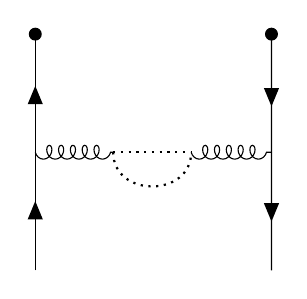
\begin{tikzpicture}[transform shape,scale=1,baseline=($(a)!0.5!(exa)$.base)]
			\begin{feynman}
				\node[dot] (a);
				\node[right=\FDWidth of a,dot] (b);
				\vertex[below=\FDHeight of a] (exa);
				\vertex[below=\FDHeight of b] (exb);
				% 
				\vertex at ($(a)!0.33!(b)$) (o13);
				\vertex at ($(a)!0.66!(b)$) (o23);
				\vertex at ($(a)!0.25!(b)$) (o14);
				\vertex at ($(a)!0.5!(b)$) (o12);
				\vertex at ($(a)!0.75!(b)$) (o34);
				% 
				\vertex at ($(a)!0.2!(b)$) (o15);
				\vertex at ($(a)!0.4!(b)$) (o25);
				\vertex at ($(a)!0.6!(b)$) (o35);
				\vertex at ($(a)!0.8!(b)$) (o45);
				% HOWTO: One can modify this to get vertexes lower than the gauge link line. 
				\vertex at ($(o13)+1/4*(0,-\FDHeight)$) (o13m);
				\vertex at ($(o23)+1/4*(0,-\FDHeight)$) (o23m);
				% 
				\vertex at ($(exa)!0.25!(a)$) (a14);
				\vertex at ($(exa)!0.5!(a)$) (a12);
				\vertex at ($(exa)!0.75!(a)$) (a34);
				\vertex at ($(exa)!0.33!(a)$) (a13);
				\vertex at ($(exa)!0.66!(a)$) (a23);
				% 
				\vertex at ($(exb)!0.25!(b)$) (b14);
				\vertex at ($(exb)!0.5!(b)$) (b12);
				\vertex at ($(exb)!0.75!(b)$) (b34);
				\vertex at ($(exb)!0.33!(b)$) (b13);
				\vertex at ($(exb)!0.66!(b)$) (b23);
				% 
				\vertex at ($(a12)!0.33!(b12)$) (ab13);
				\vertex at ($(a12)!0.66!(b12)$) (ab23);
				\vertex at ($(a12)!0.5!(b12)$) (ab12);
				% 
				\vertex at ($(a14)!0.5!(a34)!1.2!-90:(a34)$) (g1);
				% 
				\diagram*{
				(exa) --[fermion] (a12) --[fermion] (a);
				(b) --[fermion] (b12) --[fermion] (exb);
				(a12) --[gluon] (ab13) --[ghost] (ab23) --[gluon] (b12);
				(ab13) --[ghost,half right] (ab23);
				};
			\end{feynman}
		\end{tikzpicture}
		\label{}
	}\hfil\null\\\null\hfil
	\subfloat[52]{
		\begin{tikzpicture}[transform shape,scale=1,baseline=($(a)!0.5!(exa)$.base)]
			\begin{feynman}
				\node[dot] (a);
				\node[right=\FDWidth of a,dot] (b);
				\vertex[below=\FDHeight of a] (exa);
				\vertex[below=\FDHeight of b] (exb);
				% 
				\vertex at ($(a)!0.33!(b)$) (o13);
				\vertex at ($(a)!0.66!(b)$) (o23);
				\vertex at ($(a)!0.25!(b)$) (o14);
				\vertex at ($(a)!0.5!(b)$) (o12);
				\vertex at ($(a)!0.75!(b)$) (o34);
				% 
				\vertex at ($(a)!0.2!(b)$) (o15);
				\vertex at ($(a)!0.4!(b)$) (o25);
				\vertex at ($(a)!0.6!(b)$) (o35);
				\vertex at ($(a)!0.8!(b)$) (o45);
				% HOWTO: One can modify this to get vertexes lower than the gauge link line. 
				\vertex at ($(o13)+1/4*(0,-\FDHeight)$) (o13m);
				\vertex at ($(o23)+1/4*(0,-\FDHeight)$) (o23m);
				% 
				\vertex at ($(exa)!0.25!(a)$) (a14);
				\vertex at ($(exa)!0.5!(a)$) (a12);
				\vertex at ($(exa)!0.75!(a)$) (a34);
				\vertex at ($(exa)!0.33!(a)$) (a13);
				\vertex at ($(exa)!0.66!(a)$) (a23);
				% 
				\vertex at ($(exb)!0.25!(b)$) (b14);
				\vertex at ($(exb)!0.5!(b)$) (b12);
				\vertex at ($(exb)!0.75!(b)$) (b34);
				\vertex at ($(exb)!0.33!(b)$) (b13);
				\vertex at ($(exb)!0.66!(b)$) (b23);
				% 
				\vertex at ($(a12)!0.33!(b12)$) (ab13);
				\vertex at ($(a12)!0.66!(b12)$) (ab23);
				\vertex at ($(a12)!0.5!(b12)$) (ab12);
				% 
				\vertex at ($(a14)!0.5!(a34)!1.2!-90:(a34)$) (g1);
				% 
				\diagram*{
				(a12) --[gluon] (o23);
				(o13) --[white,line width=3mm] (b12);;
				(a) --[Eikonal] (o13);
				(o23) --[Eikonal] (b);
				(exa) --[fermion] (a12) --[fermion] (a);
				(b) --[fermion] (b12) --[fermion] (exb);
				(o13) --[gluon] (b12);
				};
			\end{feynman}
		\end{tikzpicture}
		\label{}
	}\hfil
	\subfloat[71]{
		\begin{tikzpicture}[transform shape,scale=1,baseline=($(a)!0.5!(exa)$.base)]
			\begin{feynman}
				\node[dot] (a);
				\node[right=\FDWidth of a,dot] (b);
				\vertex[below=\FDHeight of a] (exa);
				\vertex[below=\FDHeight of b] (exb);
				% 
				\vertex at ($(a)!0.33!(b)$) (o13);
				\vertex at ($(a)!0.66!(b)$) (o23);
				\vertex at ($(a)!0.25!(b)$) (o14);
				\vertex at ($(a)!0.5!(b)$) (o12);
				\vertex at ($(a)!0.75!(b)$) (o34);
				% 
				\vertex at ($(a)!0.2!(b)$) (o15);
				\vertex at ($(a)!0.4!(b)$) (o25);
				\vertex at ($(a)!0.6!(b)$) (o35);
				\vertex at ($(a)!0.8!(b)$) (o45);
				% HOWTO: One can modify this to get vertexes lower than the gauge link line. 
				\vertex at ($(o13)+1/4*(0,-\FDHeight)$) (o13m);
				\vertex at ($(o23)+1/4*(0,-\FDHeight)$) (o23m);
				% 
				\vertex at ($(exa)!0.25!(a)$) (a14);
				\vertex at ($(exa)!0.5!(a)$) (a12);
				\vertex at ($(exa)!0.75!(a)$) (a34);
				\vertex at ($(exa)!0.33!(a)$) (a13);
				\vertex at ($(exa)!0.66!(a)$) (a23);
				% 
				\vertex at ($(exb)!0.25!(b)$) (b14);
				\vertex at ($(exb)!0.5!(b)$) (b12);
				\vertex at ($(exb)!0.75!(b)$) (b34);
				\vertex at ($(exb)!0.33!(b)$) (b13);
				\vertex at ($(exb)!0.66!(b)$) (b23);
				% 
				\vertex at ($(a12)!0.33!(b12)$) (ab13);
				\vertex at ($(a12)!0.66!(b12)$) (ab23);
				\vertex at ($(a12)!0.5!(b12)$) (ab12);
				% 
				\vertex at ($(a14)!0.5!(a34)!1.2!-90:(a34)$) (g1);
				% 
				\diagram*{
				(a) --[Eikonal] (o13);
				(o23) --[Eikonal] (b);
				(exa) --[fermion] (a12) --[fermion] (a);
				(b) --[fermion] (b12) --[fermion] (exb);
				(o13) --[gluon,half right] (o23);
				(a12) --[gluon] (b12);
				};
			\end{feynman}
		\end{tikzpicture}
		\label{}
	}\hfil
	\subfloat[87]{
		\begin{tikzpicture}[transform shape,scale=1,baseline=($(a)!0.5!(exa)$.base)]
			\begin{feynman}
				\node[dot] (a);
				\node[right=\FDWidth of a,dot] (b);
				\vertex[below=\FDHeight of a] (exa);
				\vertex[below=\FDHeight of b] (exb);
				% 
				\vertex at ($(a)!0.33!(b)$) (o13);
				\vertex at ($(a)!0.66!(b)$) (o23);
				\vertex at ($(a)!0.25!(b)$) (o14);
				\vertex at ($(a)!0.5!(b)$) (o12);
				\vertex at ($(a)!0.75!(b)$) (o34);
				% 
				\vertex at ($(a)!0.2!(b)$) (o15);
				\vertex at ($(a)!0.4!(b)$) (o25);
				\vertex at ($(a)!0.6!(b)$) (o35);
				\vertex at ($(a)!0.8!(b)$) (o45);
				% HOWTO: One can modify this to get vertexes lower than the gauge link line. 
				\vertex at ($(o13)+1/4*(0,-\FDHeight)$) (o13m);
				\vertex at ($(o23)+1/4*(0,-\FDHeight)$) (o23m);
				% 
				\vertex at ($(exa)!0.25!(a)$) (a14);
				\vertex at ($(exa)!0.5!(a)$) (a12);
				\vertex at ($(exa)!0.75!(a)$) (a34);
				\vertex at ($(exa)!0.33!(a)$) (a13);
				\vertex at ($(exa)!0.66!(a)$) (a23);
				% 
				\vertex at ($(exb)!0.25!(b)$) (b14);
				\vertex at ($(exb)!0.5!(b)$) (b12);
				\vertex at ($(exb)!0.75!(b)$) (b34);
				\vertex at ($(exb)!0.33!(b)$) (b13);
				\vertex at ($(exb)!0.66!(b)$) (b23);
				% 
				\vertex at ($(a12)!0.33!(b12)$) (ab13);
				\vertex at ($(a12)!0.66!(b12)$) (ab23);
				\vertex at ($(a12)!0.5!(b12)$) (ab12);
				% 
				\vertex at ($(a14)!0.5!(a34)!1.2!-90:(a34)$) (g1);
				% 
				\diagram*{
				(a) --[Eikonal] (o15) --[Eikonal] (o25);
				(o35) --[Eikonal] (o45) --[Eikonal] (b);
				(exa) --[fermion] (a);
				(b) --[fermion] (exb);
				(o15) --[gluon,half right] (o45);
				(o25) --[gluon,half right] (o35);
				};
			\end{feynman}
		\end{tikzpicture}
		\label{}
	}\hfil
	\subfloat[100]{
		\begin{tikzpicture}[transform shape,scale=1,baseline=($(a)!0.5!(exa)$.base)]
			\begin{feynman}
				\node[dot] (a);
				\node[right=\FDWidth of a,dot] (b);
				\vertex[below=\FDHeight of a] (exa);
				\vertex[below=\FDHeight of b] (exb);
				% 
				\vertex at ($(a)!0.33!(b)$) (o13);
				\vertex at ($(a)!0.66!(b)$) (o23);
				\vertex at ($(a)!0.25!(b)$) (o14);
				\vertex at ($(a)!0.5!(b)$) (o12);
				\vertex at ($(a)!0.75!(b)$) (o34);
				% 
				\vertex at ($(a)!0.2!(b)$) (o15);
				\vertex at ($(a)!0.4!(b)$) (o25);
				\vertex at ($(a)!0.6!(b)$) (o35);
				\vertex at ($(a)!0.8!(b)$) (o45);
				% HOWTO: One can modify this to get vertexes lower than the gauge link line. 
				\vertex at ($(o13)+1/4*(0,-\FDHeight)$) (o13m);
				\vertex at ($(o23)+1/4*(0,-\FDHeight)$) (o23m);
				% 
				\vertex at ($(exa)!0.25!(a)$) (a14);
				\vertex at ($(exa)!0.5!(a)$) (a12);
				\vertex at ($(exa)!0.75!(a)$) (a34);
				\vertex at ($(exa)!0.33!(a)$) (a13);
				\vertex at ($(exa)!0.66!(a)$) (a23);
				% 
				\vertex at ($(exb)!0.25!(b)$) (b14);
				\vertex at ($(exb)!0.5!(b)$) (b12);
				\vertex at ($(exb)!0.75!(b)$) (b34);
				\vertex at ($(exb)!0.33!(b)$) (b13);
				\vertex at ($(exb)!0.66!(b)$) (b23);
				% 
				\vertex at ($(a12)!0.33!(b12)$) (ab13);
				\vertex at ($(a12)!0.66!(b12)$) (ab23);
				\vertex at ($(a12)!0.5!(b12)$) (ab12);
				% 
				\vertex at ($(a14)!0.5!(a34)!1.2!-90:(a34)$) (g1);
				% 
				\diagram*{
				(a) --[Eikonal] (o15) --[Eikonal] (o25);
				(o35) --[Eikonal] (o45) --[Eikonal] (b);
				(exa) --[fermion] (a);
				(b) --[fermion] (exb);
				(o35) --[gluon,half right,looseness=1.5] (o15);
				(o25) --[gluon,half right,looseness=1.5] (o45);
				};
			\end{feynman}
		\end{tikzpicture}
		\label{}
	}\hfil\null\\\null\hfil
	\subfloat[116]{
		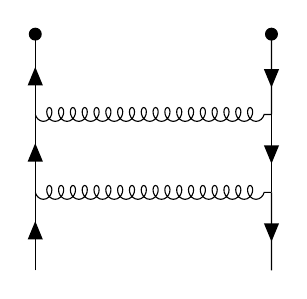
\begin{tikzpicture}[transform shape,scale=1,baseline=($(a)!0.5!(exa)$.base)]
			\begin{feynman}
				\node[dot] (a);
				\node[right=\FDWidth of a,dot] (b);
				\vertex[below=\FDHeight of a] (exa);
				\vertex[below=\FDHeight of b] (exb);
				% 
				\vertex at ($(a)!0.33!(b)$) (o13);
				\vertex at ($(a)!0.66!(b)$) (o23);
				\vertex at ($(a)!0.25!(b)$) (o14);
				\vertex at ($(a)!0.5!(b)$) (o12);
				\vertex at ($(a)!0.75!(b)$) (o34);
				% 
				\vertex at ($(a)!0.2!(b)$) (o15);
				\vertex at ($(a)!0.4!(b)$) (o25);
				\vertex at ($(a)!0.6!(b)$) (o35);
				\vertex at ($(a)!0.8!(b)$) (o45);
				% HOWTO: One can modify this to get vertexes lower than the gauge link line. 
				\vertex at ($(o13)+1/4*(0,-\FDHeight)$) (o13m);
				\vertex at ($(o23)+1/4*(0,-\FDHeight)$) (o23m);
				% 
				\vertex at ($(exa)!0.25!(a)$) (a14);
				\vertex at ($(exa)!0.5!(a)$) (a12);
				\vertex at ($(exa)!0.75!(a)$) (a34);
				\vertex at ($(exa)!0.33!(a)$) (a13);
				\vertex at ($(exa)!0.66!(a)$) (a23);
				% 
				\vertex at ($(exb)!0.25!(b)$) (b14);
				\vertex at ($(exb)!0.5!(b)$) (b12);
				\vertex at ($(exb)!0.75!(b)$) (b34);
				\vertex at ($(exb)!0.33!(b)$) (b13);
				\vertex at ($(exb)!0.66!(b)$) (b23);
				% 
				\vertex at ($(a12)!0.33!(b12)$) (ab13);
				\vertex at ($(a12)!0.66!(b12)$) (ab23);
				\vertex at ($(a12)!0.5!(b12)$) (ab12);
				% 
				\vertex at ($(a14)!0.5!(a34)!1.2!-90:(a34)$) (g1);
				% 
				\diagram*{
				(exa) --[fermion] (a13) --[fermion] (a23) --[fermion] (a);
				(b) --[fermion] (b23) --[fermion] (b13) --[fermion] (exb);
				(a13) --[gluon] (b13);
				(a23) --[gluon] (b23);
				};
			\end{feynman}
		\end{tikzpicture}
		\label{}
	}\hfil
	\subfloat[124\red{/4.12}]{
		\begin{tikzpicture}[transform shape,scale=1,baseline=($(a)!0.5!(exa)$.base)]
			\begin{feynman}
				\node[dot] (a);
				\node[right=\FDWidth of a,dot] (b);
				\vertex[below=\FDHeight of a] (exa);
				\vertex[below=\FDHeight of b] (exb);
				% 
				\vertex at ($(a)!0.33!(b)$) (o13);
				\vertex at ($(a)!0.66!(b)$) (o23);
				\vertex at ($(a)!0.25!(b)$) (o14);
				\vertex at ($(a)!0.5!(b)$) (o12);
				\vertex at ($(a)!0.75!(b)$) (o34);
				% 
				\vertex at ($(a)!0.2!(b)$) (o15);
				\vertex at ($(a)!0.4!(b)$) (o25);
				\vertex at ($(a)!0.6!(b)$) (o35);
				\vertex at ($(a)!0.8!(b)$) (o45);
				% 
				\vertex at ($(o13)+1/4*(0,-\FDHeight)$) (o13m);
				\vertex at ($(o23)+1/4*(0,-\FDHeight)$) (o23m);
				% 
				\vertex at ($(exa)!0.25!(a)$) (a14);
				\vertex at ($(exa)!0.5!(a)$) (a12);
				\vertex at ($(exa)!0.75!(a)$) (a34);
				\vertex at ($(exa)!0.33!(a)$) (a13);
				\vertex at ($(exa)!0.66!(a)$) (a23);
				% 
				\vertex at ($(exb)!0.25!(b)$) (b14);
				\vertex at ($(exb)!0.5!(b)$) (b12);
				\vertex at ($(exb)!0.75!(b)$) (b34);
				\vertex at ($(exb)!0.33!(b)$) (b13);
				\vertex at ($(exb)!0.66!(b)$) (b23);
				% 
				\vertex at ($(a12)!0.33!(b12)$) (ab13);
				\vertex at ($(a12)!0.66!(b12)$) (ab23);
				\vertex at ($(a12)!0.5!(b12)$) (ab12);
				% 
				\vertex at ($(a14)!0.5!(a34)!1.2!-90:(a34)$) (g1);
				% 
				\diagram*{
				(a) --[Eikonal] (o13);
				(o23) --[Eikonal] (b);
				(exa) --[fermion] (a);
				(b) --[fermion] (exb);
				(o13) --[gluon] (o13m);
				(o23) --[gluon] (o23m);
				(o13m) --[fermion] (o23m);
				(o23m) --[fermion,half left,looseness=1.5] (o13m);
				};
			\end{feynman}
		\end{tikzpicture}
		\label{}
	}\hfil
	\subfloat[125\red{/4.11}]{
		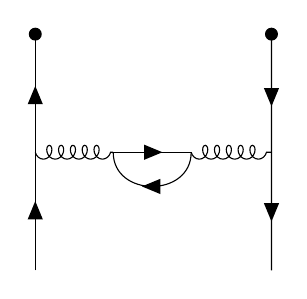
\begin{tikzpicture}[transform shape,scale=1,baseline=($(a)!0.5!(exa)$.base)]
			\begin{feynman}
				\node[dot] (a);
				\node[right=\FDWidth of a,dot] (b);
				\vertex[below=\FDHeight of a] (exa);
				\vertex[below=\FDHeight of b] (exb);
				% 
				\vertex at ($(a)!0.33!(b)$) (o13);
				\vertex at ($(a)!0.66!(b)$) (o23);
				\vertex at ($(a)!0.25!(b)$) (o14);
				\vertex at ($(a)!0.5!(b)$) (o12);
				\vertex at ($(a)!0.75!(b)$) (o34);
				% 
				\vertex at ($(a)!0.2!(b)$) (o15);
				\vertex at ($(a)!0.4!(b)$) (o25);
				\vertex at ($(a)!0.6!(b)$) (o35);
				\vertex at ($(a)!0.8!(b)$) (o45);
				% HOWTO: One can modify this to get vertexes lower than the gauge link line. 
				\vertex at ($(o13)+1/4*(0,-\FDHeight)$) (o13m);
				\vertex at ($(o23)+1/4*(0,-\FDHeight)$) (o23m);
				% 
				\vertex at ($(exa)!0.25!(a)$) (a14);
				\vertex at ($(exa)!0.5!(a)$) (a12);
				\vertex at ($(exa)!0.75!(a)$) (a34);
				\vertex at ($(exa)!0.33!(a)$) (a13);
				\vertex at ($(exa)!0.66!(a)$) (a23);
				% 
				\vertex at ($(exb)!0.25!(b)$) (b14);
				\vertex at ($(exb)!0.5!(b)$) (b12);
				\vertex at ($(exb)!0.75!(b)$) (b34);
				\vertex at ($(exb)!0.33!(b)$) (b13);
				\vertex at ($(exb)!0.66!(b)$) (b23);
				% 
				\vertex at ($(a12)!0.33!(b12)$) (ab13);
				\vertex at ($(a12)!0.66!(b12)$) (ab23);
				\vertex at ($(a12)!0.5!(b12)$) (ab12);
				% 
				\vertex at ($(a14)!0.5!(a34)!1.2!-90:(a34)$) (g1);
				% 
				\diagram*{
				(exa) --[fermion] (a12) --[fermion] (a);
				(b) --[fermion] (b12) --[fermion] (exb);
				(a12) --[gluon] (ab13) --[fermion] (ab23) --[gluon] (b12);
				(ab23) --[fermion,half left] (ab13);
				};
			\end{feynman}
		\end{tikzpicture}
		\label{}
	}\hfil
	\subfloat[128]{
		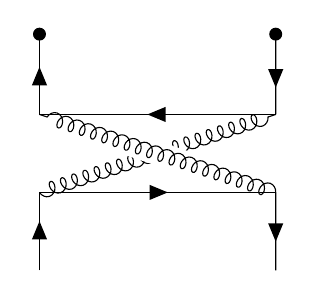
\begin{tikzpicture}[transform shape,scale=1,baseline=($(a)!0.5!(exa)$)]
			\begin{feynman}
				\node[dot] (a);
				\node[right=\FDWidth of a,dot] (b);
				\vertex[below=\FDHeight of a] (exa);
				\vertex[below=\FDHeight of b] (exb);
				% 
				\vertex at ($(a)!0.33!(b)$) (o13);
				\vertex at ($(a)!0.66!(b)$) (o23);
				\vertex at ($(a)!0.25!(b)$) (o14);
				\vertex at ($(a)!0.5!(b)$) (o12);
				\vertex at ($(a)!0.75!(b)$) (o34);
				% 
				\vertex at ($(a)!0.2!(b)$) (o15);
				\vertex at ($(a)!0.4!(b)$) (o25);
				\vertex at ($(a)!0.6!(b)$) (o35);
				\vertex at ($(a)!0.8!(b)$) (o45);
				% HOWTO: One can modify this to get vertexes lower than the gauge link line. 
				\vertex at ($(o13)+1/4*(0,-\FDHeight)$) (o13m);
				\vertex at ($(o23)+1/4*(0,-\FDHeight)$) (o23m);
				% 
				\vertex at ($(exa)!0.25!(a)$) (a14);
				\vertex at ($(exa)!0.5!(a)$) (a12);
				\vertex at ($(exa)!0.75!(a)$) (a34);
				\vertex at ($(exa)!0.33!(a)$) (a13);
				\vertex at ($(exa)!0.66!(a)$) (a23);
				% 
				\vertex at ($(exb)!0.25!(b)$) (b14);
				\vertex at ($(exb)!0.5!(b)$) (b12);
				\vertex at ($(exb)!0.75!(b)$) (b34);
				\vertex at ($(exb)!0.33!(b)$) (b13);
				\vertex at ($(exb)!0.66!(b)$) (b23);
				% 
				\vertex at ($(a12)!0.33!(b12)$) (ab13);
				\vertex at ($(a12)!0.66!(b12)$) (ab23);
				\vertex at ($(a12)!0.5!(b12)$) (ab12);
				% 
				\vertex at ($(a14)!0.5!(a34)!1.2!-90:(a34)$) (g1);
				% 
				\diagram*{
				(a13) --[gluon] (b23);
				(b13) --[white,line width=3mm] (a23);
				(b13) --[gluon] (a23);
				(exa) --[fermion] (a13) --[fermion] (b13) --[fermion] (exb);
				(b) --[fermion] (b23) --[fermion] (a23) --[fermion] (a);
				};
			\end{feynman}
		\end{tikzpicture}
		\label{}
	}\hfil
	\null\\\null\hfil
	\subfloat[129]{
		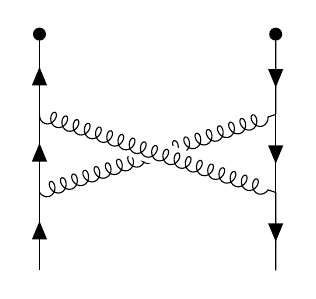
\begin{tikzpicture}[transform shape,scale=1,baseline=($(a)!0.5!(exa)$.base)]
			\begin{feynman}
				\node[dot] (a);
				\node[right=\FDWidth of a,dot] (b);
				\vertex[below=\FDHeight of a] (exa);
				\vertex[below=\FDHeight of b] (exb);
				% 
				\vertex at ($(a)!0.33!(b)$) (o13);
				\vertex at ($(a)!0.66!(b)$) (o23);
				\vertex at ($(a)!0.25!(b)$) (o14);
				\vertex at ($(a)!0.5!(b)$) (o12);
				\vertex at ($(a)!0.75!(b)$) (o34);
				% 
				\vertex at ($(a)!0.2!(b)$) (o15);
				\vertex at ($(a)!0.4!(b)$) (o25);
				\vertex at ($(a)!0.6!(b)$) (o35);
				\vertex at ($(a)!0.8!(b)$) (o45);
				% HOWTO: One can modify this to get vertexes lower than the gauge link line. 
				\vertex at ($(o13)+1/4*(0,-\FDHeight)$) (o13m);
				\vertex at ($(o23)+1/4*(0,-\FDHeight)$) (o23m);
				% 
				\vertex at ($(exa)!0.25!(a)$) (a14);
				\vertex at ($(exa)!0.5!(a)$) (a12);
				\vertex at ($(exa)!0.75!(a)$) (a34);
				\vertex at ($(exa)!0.33!(a)$) (a13);
				\vertex at ($(exa)!0.66!(a)$) (a23);
				% 
				\vertex at ($(exb)!0.25!(b)$) (b14);
				\vertex at ($(exb)!0.5!(b)$) (b12);
				\vertex at ($(exb)!0.75!(b)$) (b34);
				\vertex at ($(exb)!0.33!(b)$) (b13);
				\vertex at ($(exb)!0.66!(b)$) (b23);
				% 
				\vertex at ($(a12)!0.33!(b12)$) (ab13);
				\vertex at ($(a12)!0.66!(b12)$) (ab23);
				\vertex at ($(a12)!0.5!(b12)$) (ab12);
				% 
				\vertex at ($(a14)!0.5!(a34)!1.2!-90:(a34)$) (g1);
				% 
				\diagram*{
				(a13) --[gluon] (b23);
				(a23) --[white, line width=3mm] (b13);
				(exa) --[fermion] (a13) --[fermion] (a23) --[fermion] (a);
				(b) --[fermion] (b23) --[fermion] (b13) --[fermion] (exb);
				(a23) --[gluon] (b13);
				};
			\end{feynman}
		\end{tikzpicture}
		\label{}
	}\hfil
	\subfloat[133]{
		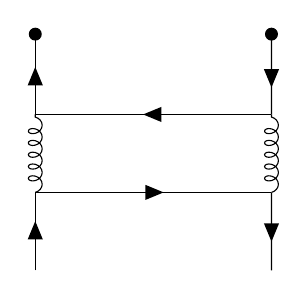
\begin{tikzpicture}[transform shape,scale=1,baseline=($(a)!0.5!(exa)$.base)]
			\begin{feynman}
				\node[dot] (a);
				\node[right=\FDWidth of a,dot] (b);
				\vertex[below=\FDHeight of a] (exa);
				\vertex[below=\FDHeight of b] (exb);
				% 
				\vertex at ($(a)!0.33!(b)$) (o13);
				\vertex at ($(a)!0.66!(b)$) (o23);
				\vertex at ($(a)!0.25!(b)$) (o14);
				\vertex at ($(a)!0.5!(b)$) (o12);
				\vertex at ($(a)!0.75!(b)$) (o34);
				% 
				\vertex at ($(a)!0.2!(b)$) (o15);
				\vertex at ($(a)!0.4!(b)$) (o25);
				\vertex at ($(a)!0.6!(b)$) (o35);
				\vertex at ($(a)!0.8!(b)$) (o45);
				% HOWTO: One can modify this to get vertexes lower than the gauge link line. 
				\vertex at ($(o13)+1/4*(0,-\FDHeight)$) (o13m);
				\vertex at ($(o23)+1/4*(0,-\FDHeight)$) (o23m);
				% 
				\vertex at ($(exa)!0.25!(a)$) (a14);
				\vertex at ($(exa)!0.5!(a)$) (a12);
				\vertex at ($(exa)!0.75!(a)$) (a34);
				\vertex at ($(exa)!0.33!(a)$) (a13);
				\vertex at ($(exa)!0.66!(a)$) (a23);
				% 
				\vertex at ($(exb)!0.25!(b)$) (b14);
				\vertex at ($(exb)!0.5!(b)$) (b12);
				\vertex at ($(exb)!0.75!(b)$) (b34);
				\vertex at ($(exb)!0.33!(b)$) (b13);
				\vertex at ($(exb)!0.66!(b)$) (b23);
				% 
				\vertex at ($(a12)!0.33!(b12)$) (ab13);
				\vertex at ($(a12)!0.66!(b12)$) (ab23);
				\vertex at ($(a12)!0.5!(b12)$) (ab12);
				% 
				\vertex at ($(a14)!0.5!(a34)!1.2!-90:(a34)$) (g1);
				% 
				\diagram*{
				(exa) --[fermion] (a13) --[fermion] (b13) --[fermion] (exb);
				(b) --[fermion] (b23) --[fermion] (a23) --[fermion] (a);
				(a13) --[gluon] (a23);
				(b13) --[gluon] (b23);
				};
			\end{feynman}
		\end{tikzpicture}
		\label{}
	}\hfil\subfloat[143\red{/4.12}]{
		\begin{tikzpicture}[transform shape,scale=1,baseline=($(a)!0.5!(exa)$.base)]
			\begin{feynman}
				\node[dot] (a);
				\node[right=\FDWidth of a,dot] (b);
				\vertex[below=\FDHeight of a] (exa);
				\vertex[below=\FDHeight of b] (exb);
				% 
				\vertex at ($(a)!0.33!(b)$) (o13);
				\vertex at ($(a)!0.66!(b)$) (o23);
				\vertex at ($(a)!0.25!(b)$) (o14);
				\vertex at ($(a)!0.5!(b)$) (o12);
				\vertex at ($(a)!0.75!(b)$) (o34);
				% 
				\vertex at ($(a)!0.2!(b)$) (o15);
				\vertex at ($(a)!0.4!(b)$) (o25);
				\vertex at ($(a)!0.6!(b)$) (o35);
				\vertex at ($(a)!0.8!(b)$) (o45);
				% HOWTO: One can modify this to get vertexes lower than the gauge link line. 
				\vertex at ($(o13)+1/4*(0,-\FDHeight)$) (o13m);
				\vertex at ($(o23)+1/4*(0,-\FDHeight)$) (o23m);
				% 
				\vertex at ($(exa)!0.25!(a)$) (a14);
				\vertex at ($(exa)!0.5!(a)$) (a12);
				\vertex at ($(exa)!0.75!(a)$) (a34);
				\vertex at ($(exa)!0.33!(a)$) (a13);
				\vertex at ($(exa)!0.66!(a)$) (a23);
				% 
				\vertex at ($(exb)!0.25!(b)$) (b14);
				\vertex at ($(exb)!0.5!(b)$) (b12);
				\vertex at ($(exb)!0.75!(b)$) (b34);
				\vertex at ($(exb)!0.33!(b)$) (b13);
				\vertex at ($(exb)!0.66!(b)$) (b23);
				% 
				\vertex at ($(a12)!0.33!(b12)$) (ab13);
				\vertex at ($(a12)!0.66!(b12)$) (ab23);
				\vertex at ($(a12)!0.5!(b12)$) (ab12);
				% 
				\vertex at ($(o12)!1.3!-90:(o23)$) (g1);
				\vertex at ($(g1)+1/4*(0,-\FDHeight)$) (gtad);
				% 
				\diagram*{
				(a) --[Eikonal] (o13);
				(o23) --[Eikonal] (b);
				(exa) --[fermion] (a);
				(b) --[fermion] (exb);
				(o13) --[gluon,half right] (o23);
				(g1) --[gluon,out=-135,in=180] (gtad) --[gluon,out=0,in=-45] (g1);
				};
			\end{feynman}
		\end{tikzpicture}
		\label{re:143}
	}\hfil
	\subfloat[144\red{/4.11}]{
		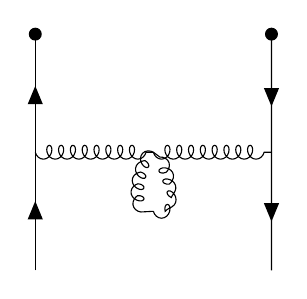
\begin{tikzpicture}[transform shape,scale=1,baseline=($(a)!0.5!(exa)$.base)]
			\begin{feynman}
				\node[dot] (a);
				\node[right=\FDWidth of a,dot] (b);
				\vertex[below=\FDHeight of a] (exa);
				\vertex[below=\FDHeight of b] (exb);
				% 
				\vertex at ($(a)!0.33!(b)$) (o13);
				\vertex at ($(a)!0.66!(b)$) (o23);
				\vertex at ($(a)!0.25!(b)$) (o14);
				\vertex at ($(a)!0.5!(b)$) (o12);
				\vertex at ($(a)!0.75!(b)$) (o34);
				% 
				\vertex at ($(a)!0.2!(b)$) (o15);
				\vertex at ($(a)!0.4!(b)$) (o25);
				\vertex at ($(a)!0.6!(b)$) (o35);
				\vertex at ($(a)!0.8!(b)$) (o45);
				% HOWTO: One can modify this to get vertexes lower than the gauge link line. 
				\vertex at ($(o13)+1/4*(0,-\FDHeight)$) (o13m);
				\vertex at ($(o23)+1/4*(0,-\FDHeight)$) (o23m);
				% 
				\vertex at ($(exa)!0.25!(a)$) (a14);
				\vertex at ($(exa)!0.5!(a)$) (a12);
				\vertex at ($(exa)!0.75!(a)$) (a34);
				\vertex at ($(exa)!0.33!(a)$) (a13);
				\vertex at ($(exa)!0.66!(a)$) (a23);
				% 
				\vertex at ($(exb)!0.25!(b)$) (b14);
				\vertex at ($(exb)!0.5!(b)$) (b12);
				\vertex at ($(exb)!0.75!(b)$) (b34);
				\vertex at ($(exb)!0.33!(b)$) (b13);
				\vertex at ($(exb)!0.66!(b)$) (b23);
				% 
				\vertex at ($(a12)!0.33!(b12)$) (ab13);
				\vertex at ($(a12)!0.66!(b12)$) (ab23);
				\vertex at ($(a12)!0.5!(b12)$) (ab12);
				% 
				\vertex at ($(ab12)+1/4*(0,-\FDHeight)$) (gtad);
				% 
				\diagram*{
				(exa) --[fermion] (a12) --[fermion] (a);
				(b) --[fermion] (b12) --[fermion] (exb);
				(a12) --[gluon] (ab12) --[gluon] (b12);
				(ab12) --[gluon,out=-135,in=180] (gtad) --[gluon,out=0,in=-45] (ab12);
				};
			\end{feynman}
		\end{tikzpicture}
		\label{}
	}\hfil\null
	\caption{All self-conjugated diagrams, \red{red n.i marks the diagram number in Ji\&Zhang's paper}. }
	\label{re:sc}
\end{figure}
\begin{figure}[!htbp]
	\centering\null\hfil
	\subfloat[2\CJ{/1}]{
		\centering
		\begin{tikzpicture}[transform shape,scale=1,baseline=($(a)!0.5!(exa)$.base)]
			\begin{feynman}
				\node[dot] (a);
				\node[right=\FDWidth of a,dot] (b);
				\vertex[below=\FDHeight of a] (exa);
				\vertex[below=\FDHeight of b] (exb);
				% 
				\vertex at ($(a)!0.33!(b)$) (o13);
				\vertex at ($(a)!0.66!(b)$) (o23);
				\vertex at ($(a)!0.25!(b)$) (o14);
				\vertex at ($(a)!0.5!(b)$) (o12);
				\vertex at ($(a)!0.75!(b)$) (o34);
				% 
				\vertex at ($(exa)!0.25!(a)$) (a14);
				\vertex at ($(exa)!0.5!(a)$) (a12);
				\vertex at ($(exa)!0.75!(a)$) (a34);
				% 
				\vertex at ($(exb)!0.25!(b)$) (b14);
				\vertex at ($(exb)!0.5!(b)$) (b12);
				\vertex at ($(exb)!0.75!(b)$) (b34);
				% 
				\vertex at ($(a12)!0.33!(b12)$) (ab13);
				\vertex at ($(a12)!0.66!(b12)$) (ab23);
				\vertex at ($(a12)!0.5!(b12)$) (ab12);
				% 
				\vertex at ($(a14)!0.5!(a34)!1.2!-90:(a34)$) (g1);
				\vertex at ($(a12)!0.5!(o23)$) (g2);
				% 
				\diagram*{
				(a) --[Eikonal] (o13);
				(o23) --[Eikonal] (b);
				(exa) --[fermion] (a12) --[fermion] (a);
				(b) --[fermion] (exb);
				(o13) --[gluon] (ab13) --[gluon] (a12);
				(o23) --[gluon] (ab13);
				};
			\end{feynman}
		\end{tikzpicture}
		\label{}
	}\hfil
	\subfloat[3\CJ{/83}]{
		\centering
		\begin{tikzpicture}[transform shape,scale=1,baseline=($(a)!0.5!(exa)$.base)]
			\begin{feynman}
				\node[dot] (a);
				\node[right=\FDWidth of a,dot] (b);
				\vertex[below=\FDHeight of a] (exa);
				\vertex[below=\FDHeight of b] (exb);
				% 
				\vertex at ($(a)!0.33!(b)$) (o13);
				\vertex at ($(a)!0.66!(b)$) (o23);
				\vertex at ($(a)!0.25!(b)$) (o14);
				\vertex at ($(a)!0.5!(b)$) (o12);
				\vertex at ($(a)!0.75!(b)$) (o34);
				% 
				\vertex at ($(exa)!0.25!(a)$) (a14);
				\vertex at ($(exa)!0.5!(a)$) (a12);
				\vertex at ($(exa)!0.75!(a)$) (a34);
				% 
				\vertex at ($(exb)!0.25!(b)$) (b14);
				\vertex at ($(exb)!0.5!(b)$) (b12);
				\vertex at ($(exb)!0.75!(b)$) (b34);
				% 
				\vertex at ($(a12)!0.33!(b12)$) (ab13);
				\vertex at ($(a12)!0.66!(b12)$) (ab23);
				\vertex at ($(a12)!0.5!(b12)$) (ab12);
				% 
				\vertex at ($(a14)!0.5!(a34)!1.2!-90:(a34)$) (g1);
				% 
				\diagram*{
				(a) --[Eikonal] (o12);
				(exa) --[fermion] (a12) --[fermion] (a);
				(b) --[fermion] (b12) --[fermion] (exb);
				(o12) --[gluon] (ab12);
				(a12) --[gluon] (ab12) --[gluon] (b12);
				};
			\end{feynman}
		\end{tikzpicture}
		\label{}
	}\hfil
	\subfloat[85\CJ{/4}\red{/3.13}]{
		\begin{tikzpicture}[transform shape,scale=1,baseline=($(a)!0.5!(exa)$.base)]
			\begin{feynman}
				\node[dot] (a);
				\node[right=\FDWidth of a,dot] (b);
				\vertex[below=\FDHeight of a] (exa);
				\vertex[below=\FDHeight of b] (exb);
				% 
				\vertex at ($(a)!0.33!(b)$) (o13);
				\vertex at ($(a)!0.66!(b)$) (o23);
				\vertex at ($(a)!0.25!(b)$) (o14);
				\vertex at ($(a)!0.5!(b)$) (o12);
				\vertex at ($(a)!0.75!(b)$) (o34);
				% 
				\vertex at ($(exa)!0.25!(a)$) (a14);
				\vertex at ($(exa)!0.5!(a)$) (a12);
				\vertex at ($(exa)!0.75!(a)$) (a34);
				% 
				\vertex at ($(exb)!0.25!(b)$) (b14);
				\vertex at ($(exb)!0.5!(b)$) (b12);
				\vertex at ($(exb)!0.75!(b)$) (b34);
				% 
				\vertex at ($(a12)!0.33!(b12)$) (ab13);
				\vertex at ($(a12)!0.66!(b12)$) (ab23);
				\vertex at ($(a12)!0.5!(b12)$) (ab12);
				% 
				\vertex at ($(a14)!0.5!(a34)!1.2!-90:(a34)$) (g1);
				% 
				\diagram*{
				(o13) --[Eikonal] (o23) --[Eikonal] (b);
				(exa) --[fermion] (a12) --[fermion] (a);
				(b) --[fermion] (exb);
				(o13) --[gluon] (ab13) --[gluon] (a12);
				(ab13) --[gluon] (o23);
				};
			\end{feynman}
		\end{tikzpicture}
		\label{}
	}\hfil
	\subfloat[5\CJ{/113}\red{/3.10}]{
		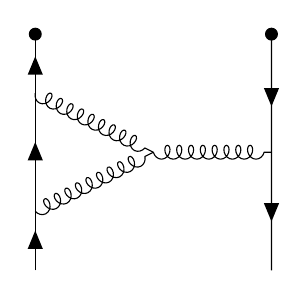
\begin{tikzpicture}[transform shape,scale=1,baseline=($(a)!0.5!(exa)$.base)]
			\begin{feynman}
				\node[dot] (a);
				\node[right=\FDWidth of a,dot] (b);
				\vertex[below=\FDHeight of a] (exa);
				\vertex[below=\FDHeight of b] (exb);
				% 
				\vertex at ($(a)!0.33!(b)$) (o13);
				\vertex at ($(a)!0.66!(b)$) (o23);
				\vertex at ($(a)!0.25!(b)$) (o14);
				\vertex at ($(a)!0.5!(b)$) (o12);
				\vertex at ($(a)!0.75!(b)$) (o34);
				% 
				\vertex at ($(exa)!0.25!(a)$) (a14);
				\vertex at ($(exa)!0.5!(a)$) (a12);
				\vertex at ($(exa)!0.75!(a)$) (a34);
				% 
				\vertex at ($(exb)!0.25!(b)$) (b14);
				\vertex at ($(exb)!0.5!(b)$) (b12);
				\vertex at ($(exb)!0.75!(b)$) (b34);
				% 
				\vertex at ($(a12)!0.33!(b12)$) (ab13);
				\vertex at ($(a12)!0.66!(b12)$) (ab23);
				\vertex at ($(a12)!0.5!(b12)$) (ab12);
				% 
				\vertex at ($(a14)!0.5!(a34)!1.2!-90:(a34)$) (g1);
				% 
				\diagram*{
				(exa) --[fermion] (a14) --[fermion] (a34) --[fermion] (a);
				(b) --[fermion] (b12) --[fermion] (exb);
				(a14) --[gluon] (ab12) --[gluon] (b12);
				(a34) --[gluon] (ab12);
				};
			\end{feynman}
		\end{tikzpicture}
		\label{}
	}\hfil\null\null\\\hfil
	\subfloat[7\CJ{/6}\red{/4.9}]{
		\begin{tikzpicture}[transform shape,scale=1,baseline=($(a)!0.5!(exa)$.base)]
			\begin{feynman}
				\node[dot] (a);
				\node[right=\FDWidth of a,dot] (b);
				\vertex[below=\FDHeight of a] (exa);
				\vertex[below=\FDHeight of b] (exb);
				% 
				\vertex at ($(a)!0.33!(b)$) (o13);
				\vertex at ($(a)!0.66!(b)$) (o23);
				\vertex at ($(a)!0.25!(b)$) (o14);
				\vertex at ($(a)!0.5!(b)$) (o12);
				\vertex at ($(a)!0.75!(b)$) (o34);
				% 
				\vertex at ($(exa)!0.25!(a)$) (a14);
				\vertex at ($(exa)!0.5!(a)$) (a12);
				\vertex at ($(exa)!0.75!(a)$) (a34);
				% 
				\vertex at ($(exb)!0.25!(b)$) (b14);
				\vertex at ($(exb)!0.5!(b)$) (b12);
				\vertex at ($(exb)!0.75!(b)$) (b34);
				% 
				\vertex at ($(a12)!0.33!(b12)$) (ab13);
				\vertex at ($(a12)!0.66!(b12)$) (ab23);
				\vertex at ($(a12)!0.5!(b12)$) (ab12);
				% 
				\vertex at ($(a14)!0.5!(a34)!1.2!-90:(a34)$) (g1);
				\vertex at ($(ab12)+(0,1/5*\FDHeight)$) (ab123);
				% 
				\diagram*{
				(a) --[Eikonal] (o14);
				(o12) --[Eikonal] (o34) --[Eikonal] (b);
				(exa) --[fermion] (a);
				(b) --[fermion] (exb);
				(o14) --[gluon, quarter right] (ab123);
				(o12) --[gluon] (ab123);
				(o34) --[gluon, quarter left] (ab123);
				};
			\end{feynman}
		\end{tikzpicture}
		\label{}
	}\hfil
	\subfloat[13\CJ{/14}\red{/4.10}]{
		\begin{tikzpicture}[transform shape,scale=1,baseline=($(a)!0.5!(exa)$.base)]
			\begin{feynman}
				\node[dot] (a);
				\node[right=\FDWidth of a,dot] (b);
				\vertex[below=\FDHeight of a] (exa);
				\vertex[below=\FDHeight of b] (exb);
				% 
				\vertex at ($(a)!0.33!(b)$) (o13);
				\vertex at ($(a)!0.66!(b)$) (o23);
				\vertex at ($(a)!0.25!(b)$) (o14);
				\vertex at ($(a)!0.5!(b)$) (o12);
				\vertex at ($(a)!0.75!(b)$) (o34);
				% 
				\vertex at ($(exa)!0.25!(a)$) (a14);
				\vertex at ($(exa)!0.5!(a)$) (a12);
				\vertex at ($(exa)!0.75!(a)$) (a34);
				% 
				\vertex at ($(exb)!0.25!(b)$) (b14);
				\vertex at ($(exb)!0.5!(b)$) (b12);
				\vertex at ($(exb)!0.75!(b)$) (b34);
				% 
				\vertex at ($(a12)!0.33!(b12)$) (ab13);
				\vertex at ($(a12)!0.66!(b12)$) (ab23);
				\vertex at ($(a12)!0.5!(b12)$) (ab12);
				% 
				\vertex at ($(a14)!0.5!(a34)!1.2!-90:(a34)$) (g1);
				\vertex at ($(o12)!0.66!(a12)$) (g13);
				\vertex at ($(o12)!0.33!(a12)$) (g23);
				% 
				\diagram*{
				(o12) --[Eikonal] (b);
				(exa) --[fermion] (a12) --[fermion] (a);
				(b) --[fermion] (exb);
				(a12) --[gluon] (g13);
				(g13) --[gluon] (g23);
				(g23) --[gluon] (o12);
				(g13) --[gluon,half right] (g23);
				};
			\end{feynman}
		\end{tikzpicture}
		\label{}
	}\hfil
	\subfloat[16\CJ{/18}\red{/3.7}]{
		\begin{tikzpicture}[transform shape,scale=1,baseline=($(a)!0.5!(exa)$.base)]
			\begin{feynman}
				\node[dot] (a);
				\node[right=\FDWidth of a,dot] (b);
				\vertex[below=\FDHeight of a] (exa);
				\vertex[below=\FDHeight of b] (exb);
				% 
				\vertex at ($(a)!0.33!(b)$) (o13);
				\vertex at ($(a)!0.66!(b)$) (o23);
				\vertex at ($(a)!0.25!(b)$) (o14);
				\vertex at ($(a)!0.5!(b)$) (o12);
				\vertex at ($(a)!0.75!(b)$) (o34);
				% 
				\vertex at ($(exa)!0.25!(a)$) (a14);
				\vertex at ($(exa)!0.5!(a)$) (a12);
				\vertex at ($(exa)!0.75!(a)$) (a34);
				% 
				\vertex at ($(exb)!0.25!(b)$) (b14);
				\vertex at ($(exb)!0.5!(b)$) (b12);
				\vertex at ($(exb)!0.75!(b)$) (b34);
				% 
				\vertex at ($(a12)!0.33!(b12)$) (ab13);
				\vertex at ($(a12)!0.66!(b12)$) (ab23);
				\vertex at ($(a12)!0.5!(b12)$) (ab12);
				% 
				\vertex at ($(a14)!0.5!(a34)!1.2!-90:(a34)$) (g1);
				% 
				\diagram*{
				(o12) --[Eikonal] (b);
				(exa) --[fermion] (a14) --[fermion] (a34) --[fermion] (a);
				(b) --[fermion] (exb);
				(a14) --[gluon] (ab12);
				(a34) --[gluon] (ab12);
				(o12) --[gluon] (ab12);
				};
			\end{feynman}
		\end{tikzpicture}
		\label{}
	}\hfil
	\subfloat[25\CJ{/22}\red{/4.10}]{
		\begin{tikzpicture}[transform shape,scale=1,baseline=($(a)!0.5!(exa)$.base)]
			\begin{feynman}
				\node[dot] (a);
				\node[right=\FDWidth of a,dot] (b);
				\vertex[below=\FDHeight of a] (exa);
				\vertex[below=\FDHeight of b] (exb);
				% 
				\vertex at ($(a)!0.33!(b)$) (o13);
				\vertex at ($(a)!0.66!(b)$) (o23);
				\vertex at ($(a)!0.25!(b)$) (o14);
				\vertex at ($(a)!0.5!(b)$) (o12);
				\vertex at ($(a)!0.75!(b)$) (o34);
				% 
				\vertex at ($(exa)!0.25!(a)$) (a14);
				\vertex at ($(exa)!0.5!(a)$) (a12);
				\vertex at ($(exa)!0.75!(a)$) (a34);
				% 
				\vertex at ($(exb)!0.25!(b)$) (b14);
				\vertex at ($(exb)!0.5!(b)$) (b12);
				\vertex at ($(exb)!0.75!(b)$) (b34);
				% 
				\vertex at ($(a12)!0.33!(b12)$) (ab13);
				\vertex at ($(a12)!0.66!(b12)$) (ab23);
				\vertex at ($(a12)!0.5!(b12)$) (ab12);
				% 
				\vertex at ($(a14)!0.5!(a34)!1.2!-90:(a34)$) (g1);
				\vertex at ($(o12)!0.66!(a12)$) (g13);
				\vertex at ($(o12)!0.33!(a12)$) (g23);
				% 
				\diagram*{
				(o12) --[Eikonal] (b);
				(exa) --[fermion] (a12) --[fermion] (a);
				(b) --[fermion] (exb);
				(a12) --[gluon] (g13);
				(g13) --[ghost] (g23);
				(g23) --[gluon] (o12);
				(g13) --[ghost,half right] (g23);
				};
			\end{feynman}
		\end{tikzpicture}
		\label{}
	}\hfil\null\\\null\hfil
	\subfloat[88\CJ{/30}]{
		\begin{tikzpicture}[transform shape,scale=1,baseline=($(a)!0.5!(exa)$.base)]
			\begin{feynman}
				\node[dot] (a);
				\node[right=\FDWidth of a,dot] (b);
				\vertex[below=\FDHeight of a] (exa);
				\vertex[below=\FDHeight of b] (exb);
				% 
				\vertex at ($(a)!0.33!(b)$) (o13);
				\vertex at ($(a)!0.66!(b)$) (o23);
				\vertex at ($(a)!0.25!(b)$) (o14);
				\vertex at ($(a)!0.5!(b)$) (o12);
				\vertex at ($(a)!0.75!(b)$) (o34);
				% 
				\vertex at ($(exa)!0.25!(a)$) (a14);
				\vertex at ($(exa)!0.5!(a)$) (a12);
				\vertex at ($(exa)!0.75!(a)$) (a34);
				\vertex at ($(exa)!0.33!(a)$) (a13);
				\vertex at ($(exa)!0.66!(a)$) (a23);
				% 
				\vertex at ($(exb)!0.25!(b)$) (b14);
				\vertex at ($(exb)!0.5!(b)$) (b12);
				\vertex at ($(exb)!0.75!(b)$) (b34);
				% 
				\vertex at ($(a12)!0.33!(b12)$) (ab13);
				\vertex at ($(a12)!0.66!(b12)$) (ab23);
				\vertex at ($(a12)!0.5!(b12)$) (ab12);
				% 
				\vertex at ($(a14)!0.5!(a34)!1.2!-90:(a34)$) (g1);
				% 
				\diagram*{
				(o13) --[Eikonal] (o23) --[Eikonal] (b);
				(exa) --[fermion] (a13) --[fermion] (a23) --[fermion] (a);
				(b) --[fermion] (exb);
				(a23) --[gluon] (o13);
				(a13) --[gluon] (o23);
				};
			\end{feynman}
		\end{tikzpicture}
		\label{}
	}\hfil
	\subfloat[31\CJ{/106}\red{/3.11}]{
		\begin{tikzpicture}[transform shape,scale=1,baseline=($(a)!0.5!(exa)$.base)]
			\begin{feynman}
				\node[dot] (a);
				\node[right=\FDWidth of a,dot] (b);
				\vertex[below=\FDHeight of a] (exa);
				\vertex[below=\FDHeight of b] (exb);
				% 
				\vertex at ($(a)!0.33!(b)$) (o13);
				\vertex at ($(a)!0.66!(b)$) (o23);
				\vertex at ($(a)!0.25!(b)$) (o14);
				\vertex at ($(a)!0.5!(b)$) (o12);
				\vertex at ($(a)!0.75!(b)$) (o34);
				% 
				\vertex at ($(exa)!0.25!(a)$) (a14);
				\vertex at ($(exa)!0.5!(a)$) (a12);
				\vertex at ($(exa)!0.75!(a)$) (a34);
				\vertex at ($(exa)!0.33!(a)$) (a13);
				\vertex at ($(exa)!0.66!(a)$) (a23);
				% 
				\vertex at ($(exb)!0.25!(b)$) (b14);
				\vertex at ($(exb)!0.5!(b)$) (b12);
				\vertex at ($(exb)!0.75!(b)$) (b34);
				% 
				\vertex at ($(a12)!0.33!(b12)$) (ab13);
				\vertex at ($(a12)!0.66!(b12)$) (ab23);
				\vertex at ($(a12)!0.5!(b12)$) (ab12);
				% 
				\vertex at ($(a14)!0.5!(a34)!1.2!-90:(a34)$) (g1);
				% 
				\diagram*{
				(a) --[Eikonal] (o13);
				(o23) --[Eikonal] (b);
				(exa) --[fermion] (a13) --[fermion] (a23) --[fermion] (a);
				(b) --[fermion] (exb);
				(a23) --[gluon] (o13);
				(a13) --[gluon] (o23);
				};
			\end{feynman}
		\end{tikzpicture}
		\label{}
	}\hfil
	\subfloat[32\CJ{/82}\red{/3.12}]{
		\begin{tikzpicture}[transform shape,scale=1,baseline=($(a)!0.5!(exa)$.base)]
			\begin{feynman}
				\node[dot] (a);
				\node[right=\FDWidth of a,dot] (b);
				\vertex[below=\FDHeight of a] (exa);
				\vertex[below=\FDHeight of b] (exb);
				% 
				\vertex at ($(a)!0.33!(b)$) (o13);
				\vertex at ($(a)!0.66!(b)$) (o23);
				\vertex at ($(a)!0.25!(b)$) (o14);
				\vertex at ($(a)!0.5!(b)$) (o12);
				\vertex at ($(a)!0.75!(b)$) (o34);
				% 
				\vertex at ($(exa)!0.25!(a)$) (a14);
				\vertex at ($(exa)!0.5!(a)$) (a12);
				\vertex at ($(exa)!0.75!(a)$) (a34);
				\vertex at ($(exa)!0.33!(a)$) (a13);
				\vertex at ($(exa)!0.66!(a)$) (a23);
				% 
				\vertex at ($(exb)!0.25!(b)$) (b14);
				\vertex at ($(exb)!0.5!(b)$) (b12);
				\vertex at ($(exb)!0.75!(b)$) (b34);
				\vertex at ($(exb)!0.33!(b)$) (b13);
				\vertex at ($(exb)!0.66!(b)$) (b23);
				% 
				\vertex at ($(a12)!0.33!(b12)$) (ab13);
				\vertex at ($(a12)!0.66!(b12)$) (ab23);
				\vertex at ($(a12)!0.5!(b12)$) (ab12);
				% 
				\vertex at ($(a14)!0.5!(a34)!1.2!-90:(a34)$) (g1);
				% 
				\diagram*{
				(a) --[Eikonal] (o13);
				(exa) --[fermion] (a13) --[fermion] (a23) --[fermion] (a);
				(b)  --[fermion] (b13)--[fermion] (exb);
				(a23) --[gluon] (o13);
				(a13) --[gluon] (b13);
				};
			\end{feynman}
		\end{tikzpicture}
		\label{}
	}\hfil
	\subfloat[38\CJ{/62}]{
		\begin{tikzpicture}[transform shape,scale=1,baseline=($(a)!0.5!(exa)$.base)]
			\begin{feynman}
				\node[dot] (a);
				\node[right=\FDWidth of a,dot] (b);
				\vertex[below=\FDHeight of a] (exa);
				\vertex[below=\FDHeight of b] (exb);
				% 
				\vertex at ($(a)!0.33!(b)$) (o13);
				\vertex at ($(a)!0.66!(b)$) (o23);
				\vertex at ($(a)!0.25!(b)$) (o14);
				\vertex at ($(a)!0.5!(b)$) (o12);
				\vertex at ($(a)!0.75!(b)$) (o34);
				% 
				\vertex at ($(exa)!0.25!(a)$) (a14);
				\vertex at ($(exa)!0.5!(a)$) (a12);
				\vertex at ($(exa)!0.75!(a)$) (a34);
				\vertex at ($(exa)!0.33!(a)$) (a13);
				\vertex at ($(exa)!0.66!(a)$) (a23);
				% 
				\vertex at ($(exb)!0.25!(b)$) (b14);
				\vertex at ($(exb)!0.5!(b)$) (b12);
				\vertex at ($(exb)!0.75!(b)$) (b34);
				% 
				\vertex at ($(a12)!0.33!(b12)$) (ab13);
				\vertex at ($(a12)!0.66!(b12)$) (ab23);
				\vertex at ($(a12)!0.5!(b12)$) (ab12);
				% 
				\vertex at ($(a14)!0.5!(a34)!1.2!-90:(a34)$) (g1);
				% 
				\diagram*{
				(a) --[Eikonal] (o14);
				(o12) --[Eikonal] (o34) --[Eikonal] (b);
				(exa) --[fermion] (a12) --[fermion] (a);
				(b) --[fermion] (exb);
				(a12) --[gluon] (o12);
				(o34) --[gluon,half right,looseness=1.5] (o14);
				};
			\end{feynman}
		\end{tikzpicture}
		\label{}
	}\hfil\null\\\null\hfil
	\subfloat[89\CJ{/39}]{
		\begin{tikzpicture}[transform shape,scale=1,baseline=($(a)!0.5!(exa)$.base)]
			\begin{feynman}
				\node[dot] (a);
				\node[right=\FDWidth of a,dot] (b);
				\vertex[below=\FDHeight of a] (exa);
				\vertex[below=\FDHeight of b] (exb);
				% 
				\vertex at ($(a)!0.33!(b)$) (o13);
				\vertex at ($(a)!0.66!(b)$) (o23);
				\vertex at ($(a)!0.25!(b)$) (o14);
				\vertex at ($(a)!0.5!(b)$) (o12);
				\vertex at ($(a)!0.75!(b)$) (o34);
				% 
				\vertex at ($(exa)!0.25!(a)$) (a14);
				\vertex at ($(exa)!0.5!(a)$) (a12);
				\vertex at ($(exa)!0.75!(a)$) (a34);
				\vertex at ($(exa)!0.33!(a)$) (a13);
				\vertex at ($(exa)!0.66!(a)$) (a23);
				% 
				\vertex at ($(exb)!0.25!(b)$) (b14);
				\vertex at ($(exb)!0.5!(b)$) (b12);
				\vertex at ($(exb)!0.75!(b)$) (b34);
				\vertex at ($(exb)!0.33!(b)$) (b13);
				\vertex at ($(exb)!0.66!(b)$) (b23);
				% 
				\vertex at ($(a12)!0.33!(b12)$) (ab13);
				\vertex at ($(a12)!0.66!(b12)$) (ab23);
				\vertex at ($(a12)!0.5!(b12)$) (ab12);
				% 
				\vertex at ($(a14)!0.5!(a34)!1.2!-90:(a34)$) (g1);
				% 
				\diagram*{
				(a) --[Eikonal] (o14);
				(o12)--[Eikonal] (o34) --[Eikonal] (b);
				(exa) --[fermion] (a12) --[fermion] (a);
				(b) --[fermion] (exb);
				(o14) --[gluon,half right] (o12);
				(a12) --[gluon,quarter right,looseness=0.8] (o34);
				};
			\end{feynman}
		\end{tikzpicture}
		\label{}
	}\hfil
	\subfloat[40\CJ{/97}\red{/3.15}]{
		\begin{tikzpicture}[transform shape,scale=1,baseline=($(a)!0.5!(exa)$.base)]
			\begin{feynman}
				\node[dot] (a);
				\node[right=\FDWidth of a,dot] (b);
				\vertex[below=\FDHeight of a] (exa);
				\vertex[below=\FDHeight of b] (exb);
				% 
				\vertex at ($(a)!0.33!(b)$) (o13);
				\vertex at ($(a)!0.66!(b)$) (o23);
				\vertex at ($(a)!0.25!(b)$) (o14);
				\vertex at ($(a)!0.5!(b)$) (o12);
				\vertex at ($(a)!0.75!(b)$) (o34);
				% 
				\vertex at ($(exa)!0.25!(a)$) (a14);
				\vertex at ($(exa)!0.5!(a)$) (a12);
				\vertex at ($(exa)!0.75!(a)$) (a34);
				\vertex at ($(exa)!0.33!(a)$) (a13);
				\vertex at ($(exa)!0.66!(a)$) (a23);
				% 
				\vertex at ($(exb)!0.25!(b)$) (b14);
				\vertex at ($(exb)!0.5!(b)$) (b12);
				\vertex at ($(exb)!0.75!(b)$) (b34);
				\vertex at ($(exb)!0.33!(b)$) (b13);
				\vertex at ($(exb)!0.66!(b)$) (b23);
				% 
				\vertex at ($(a12)!0.33!(b12)$) (ab13);
				\vertex at ($(a12)!0.66!(b12)$) (ab23);
				\vertex at ($(a12)!0.5!(b12)$) (ab12);
				% 
				\vertex at ($(a14)!0.5!(a34)!1.2!-90:(a34)$) (g1);
				% 
				\diagram*{
				(a) --[Eikonal] (o14) --[Eikonal] (o12) ;
				(o34) --[Eikonal] (b);
				(exa) --[fermion] (a12) --[fermion] (a);
				(b) --[fermion] (exb);
				(o12) --[gluon,half right] (o34);
				(a12) --[gluon] (o14);
				};
			\end{feynman}
		\end{tikzpicture}
		\label{}
	}\hfil
	\subfloat[74\CJ{/41}]{
		\begin{tikzpicture}[transform shape,scale=1,baseline=($(a)!0.5!(exa)$.base)]
			\begin{feynman}
				\node[dot] (a);
				\node[right=\FDWidth of a,dot] (b);
				\vertex[below=\FDHeight of a] (exa);
				\vertex[below=\FDHeight of b] (exb);
				% 
				\vertex at ($(a)!0.33!(b)$) (o13);
				\vertex at ($(a)!0.66!(b)$) (o23);
				\vertex at ($(a)!0.25!(b)$) (o14);
				\vertex at ($(a)!0.5!(b)$) (o12);
				\vertex at ($(a)!0.75!(b)$) (o34);
				% 
				\vertex at ($(exa)!0.25!(a)$) (a14);
				\vertex at ($(exa)!0.5!(a)$) (a12);
				\vertex at ($(exa)!0.75!(a)$) (a34);
				\vertex at ($(exa)!0.33!(a)$) (a13);
				\vertex at ($(exa)!0.66!(a)$) (a23);
				% 
				\vertex at ($(exb)!0.25!(b)$) (b14);
				\vertex at ($(exb)!0.5!(b)$) (b12);
				\vertex at ($(exb)!0.75!(b)$) (b34);
				\vertex at ($(exb)!0.33!(b)$) (b13);
				\vertex at ($(exb)!0.66!(b)$) (b23);
				% 
				\vertex at ($(a12)!0.33!(b12)$) (ab13);
				\vertex at ($(a12)!0.66!(b12)$) (ab23);
				\vertex at ($(a12)!0.5!(b12)$) (ab12);
				% 
				\vertex at ($(a14)!0.5!(a34)!1.2!-90:(a34)$) (g1);
				% 
				\diagram*{
				(a23) --[gluon] (b23);
				(a13) --[white,line width=3mm] (o12);
				(a13) --[gluon] (o12);
				(o12) --[Eikonal] (b);
				(exa) --[fermion] (a13) --[fermion] (a23) --[fermion] (a);
				(b) --[fermion] (b23) --[fermion] (exb);
				};
			\end{feynman}
		\end{tikzpicture}
		\label{}
	}\hfil
	\subfloat[54\CJ{/80}\red{/4.6}]{
		\begin{tikzpicture}[transform shape,scale=1,baseline=($(a)!0.5!(exa)$.base)]
			\begin{feynman}
				\node[dot] (a);
				\node[right=\FDWidth of a,dot] (b);
				\vertex[below=\FDHeight of a] (exa);
				\vertex[below=\FDHeight of b] (exb);
				% 
				\vertex at ($(a)!0.33!(b)$) (o13);
				\vertex at ($(a)!0.66!(b)$) (o23);
				\vertex at ($(a)!0.25!(b)$) (o14);
				\vertex at ($(a)!0.5!(b)$) (o12);
				\vertex at ($(a)!0.75!(b)$) (o34);
				% 
				\vertex at ($(a)!0.2!(b)$) (o15);
				\vertex at ($(a)!0.4!(b)$) (o25);
				\vertex at ($(a)!0.6!(b)$) (o35);
				\vertex at ($(a)!0.8!(b)$) (o45);
				% 
				\vertex at ($(exa)!0.25!(a)$) (a14);
				\vertex at ($(exa)!0.5!(a)$) (a12);
				\vertex at ($(exa)!0.75!(a)$) (a34);
				\vertex at ($(exa)!0.33!(a)$) (a13);
				\vertex at ($(exa)!0.66!(a)$) (a23);
				% 
				\vertex at ($(exb)!0.25!(b)$) (b14);
				\vertex at ($(exb)!0.5!(b)$) (b12);
				\vertex at ($(exb)!0.75!(b)$) (b34);
				\vertex at ($(exb)!0.33!(b)$) (b13);
				\vertex at ($(exb)!0.66!(b)$) (b23);
				% 
				\vertex at ($(a12)!0.33!(b12)$) (ab13);
				\vertex at ($(a12)!0.66!(b12)$) (ab23);
				\vertex at ($(a12)!0.5!(b12)$) (ab12);
				% 
				\vertex at ($(a14)!0.5!(a34)!1.2!-90:(a34)$) (g1);
				% 
				\diagram*{
				(a) --[Eikonal] (o15) --[Eikonal] (o25) --[Eikonal] (o35);
				(o45) --[Eikonal] (b);
				(exa) --[fermion] (a);
				(b) --[fermion] (exb);
				(o35) --[gluon,half right] (o45);
				(o15) --[gluon,half right] (o25);
				};
			\end{feynman}
		\end{tikzpicture}
		\label{}
	}\hfil\null\\\null\hfil
	\subfloat[81\CJ{/55}\red{/3.14}]{
		\begin{tikzpicture}[transform shape,scale=1,baseline=($(a)!0.5!(exa)$.base)]
			\begin{feynman}
				\node[dot] (a);
				\node[right=\FDWidth of a,dot] (b);
				\vertex[below=\FDHeight of a] (exa);
				\vertex[below=\FDHeight of b] (exb);
				% 
				\vertex at ($(a)!0.33!(b)$) (o13);
				\vertex at ($(a)!0.66!(b)$) (o23);
				\vertex at ($(a)!0.25!(b)$) (o14);
				\vertex at ($(a)!0.5!(b)$) (o12);
				\vertex at ($(a)!0.75!(b)$) (o34);
				% 
				\vertex at ($(a)!0.2!(b)$) (o15);
				\vertex at ($(a)!0.4!(b)$) (o25);
				\vertex at ($(a)!0.6!(b)$) (o35);
				\vertex at ($(a)!0.8!(b)$) (o45);
				% 
				\vertex at ($(exa)!0.25!(a)$) (a14);
				\vertex at ($(exa)!0.5!(a)$) (a12);
				\vertex at ($(exa)!0.75!(a)$) (a34);
				\vertex at ($(exa)!0.33!(a)$) (a13);
				\vertex at ($(exa)!0.66!(a)$) (a23);
				% 
				\vertex at ($(exb)!0.25!(b)$) (b14);
				\vertex at ($(exb)!0.5!(b)$) (b12);
				\vertex at ($(exb)!0.75!(b)$) (b34);
				\vertex at ($(exb)!0.33!(b)$) (b13);
				\vertex at ($(exb)!0.66!(b)$) (b23);
				% 
				\vertex at ($(a12)!0.33!(b12)$) (ab13);
				\vertex at ($(a12)!0.66!(b12)$) (ab23);
				\vertex at ($(a12)!0.5!(b12)$) (ab12);
				% 
				\vertex at ($(a14)!0.5!(a34)!1.2!-90:(a34)$) (g1);
				% 
				\diagram*{
				(o25) --[Eikonal] (o35) --[Eikonal] (o45) --[Eikonal] (b);
				(exa) --[fermion] (a12) --[fermion] (a);
				(b) --[fermion] (exb);
				(a12) --[gluon] (o25);
				(o35) --[gluon,half right] (o45);
				};
			\end{feynman}
		\end{tikzpicture}
		\label{}
	}\hfil
	\subfloat[84\CJ{/56}\red{/4.2}]{
		\begin{tikzpicture}[transform shape,scale=1,baseline=($(a)!0.5!(exa)$.base)]
			\begin{feynman}
				\node[dot] (a);
				\node[right=\FDWidth of a,dot] (b);
				\vertex[below=\FDHeight of a] (exa);
				\vertex[below=\FDHeight of b] (exb);
				% 
				\vertex at ($(a)!0.33!(b)$) (o13);
				\vertex at ($(a)!0.66!(b)$) (o23);
				\vertex at ($(a)!0.25!(b)$) (o14);
				\vertex at ($(a)!0.5!(b)$) (o12);
				\vertex at ($(a)!0.75!(b)$) (o34);
				% 
				\vertex at ($(a)!0.2!(b)$) (o15);
				\vertex at ($(a)!0.4!(b)$) (o25);
				\vertex at ($(a)!0.6!(b)$) (o35);
				\vertex at ($(a)!0.8!(b)$) (o45);
				% 
				\vertex at ($(exa)!0.25!(a)$) (a14);
				\vertex at ($(exa)!0.5!(a)$) (a12);
				\vertex at ($(exa)!0.75!(a)$) (a34);
				\vertex at ($(exa)!0.33!(a)$) (a13);
				\vertex at ($(exa)!0.66!(a)$) (a23);
				% 
				\vertex at ($(exb)!0.25!(b)$) (b14);
				\vertex at ($(exb)!0.5!(b)$) (b12);
				\vertex at ($(exb)!0.75!(b)$) (b34);
				\vertex at ($(exb)!0.33!(b)$) (b13);
				\vertex at ($(exb)!0.66!(b)$) (b23);
				% 
				\vertex at ($(a12)!0.33!(b12)$) (ab13);
				\vertex at ($(a12)!0.66!(b12)$) (ab23);
				\vertex at ($(a12)!0.5!(b12)$) (ab12);
				% 
				\vertex at ($(a14)!0.5!(a34)!1.2!-90:(a34)$) (g1);
				% 
				\diagram*{
				(o13) --[Eikonal] (o23) --[Eikonal] (b);
				(exa) --[fermion] (a12) --[fermion] (a);
				(b) --[fermion] (b12) --[fermion] (exb);
				(b12) --[gluon] (o23);
				(a12) --[gluon] (o13);
				};
			\end{feynman}
		\end{tikzpicture}
		\label{}
	}\hfil
	\subfloat[86\CJ{/58}\red{/4.7}]{
		\begin{tikzpicture}[transform shape,scale=1,baseline=($(a)!0.5!(exa)$.base)]
			\begin{feynman}
				\node[dot] (a);
				\node[right=\FDWidth of a,dot] (b);
				\vertex[below=\FDHeight of a] (exa);
				\vertex[below=\FDHeight of b] (exb);
				% 
				\vertex at ($(a)!0.33!(b)$) (o13);
				\vertex at ($(a)!0.66!(b)$) (o23);
				\vertex at ($(a)!0.25!(b)$) (o14);
				\vertex at ($(a)!0.5!(b)$) (o12);
				\vertex at ($(a)!0.75!(b)$) (o34);
				% 
				\vertex at ($(a)!0.2!(b)$) (o15);
				\vertex at ($(a)!0.4!(b)$) (o25);
				\vertex at ($(a)!0.6!(b)$) (o35);
				\vertex at ($(a)!0.8!(b)$) (o45);
				% 
				\vertex at ($(exa)!0.25!(a)$) (a14);
				\vertex at ($(exa)!0.5!(a)$) (a12);
				\vertex at ($(exa)!0.75!(a)$) (a34);
				\vertex at ($(exa)!0.33!(a)$) (a13);
				\vertex at ($(exa)!0.66!(a)$) (a23);
				% 
				\vertex at ($(exb)!0.25!(b)$) (b14);
				\vertex at ($(exb)!0.5!(b)$) (b12);
				\vertex at ($(exb)!0.75!(b)$) (b34);
				\vertex at ($(exb)!0.33!(b)$) (b13);
				\vertex at ($(exb)!0.66!(b)$) (b23);
				% 
				\vertex at ($(a12)!0.33!(b12)$) (ab13);
				\vertex at ($(a12)!0.66!(b12)$) (ab23);
				\vertex at ($(a12)!0.5!(b12)$) (ab12);
				% 
				\vertex at ($(a14)!0.5!(a34)!1.2!-90:(a34)$) (g1);
				% 
				\diagram*{
				(a) --[Eikonal] (o15);
				(o25) --[Eikonal] (o35) --[Eikonal] (o45) --[Eikonal] (b);
				(exa) --[fermion] (a);
				(b) --[fermion] (exb);
				(o25) --[gluon,half right] (o45);
				(o35) --[gluon,half right,looseness=1.5] (o15);
				};
			\end{feynman}
		\end{tikzpicture}
		\label{}
	}\hfil
	\subfloat[95\CJ{/59}\red{/4.1}]{
		\begin{tikzpicture}[transform shape,scale=1,baseline=($(a)!0.5!(exa)$.base)]
			\begin{feynman}
				\node[dot] (a);
				\node[right=\FDWidth of a,dot] (b);
				\vertex[below=\FDHeight of a] (exa);
				\vertex[below=\FDHeight of b] (exb);
				% 
				\vertex at ($(a)!0.33!(b)$) (o13);
				\vertex at ($(a)!0.66!(b)$) (o23);
				\vertex at ($(a)!0.25!(b)$) (o14);
				\vertex at ($(a)!0.5!(b)$) (o12);
				\vertex at ($(a)!0.75!(b)$) (o34);
				% 
				\vertex at ($(a)!0.2!(b)$) (o15);
				\vertex at ($(a)!0.4!(b)$) (o25);
				\vertex at ($(a)!0.6!(b)$) (o35);
				\vertex at ($(a)!0.8!(b)$) (o45);
				% 
				\vertex at ($(exa)!0.25!(a)$) (a14);
				\vertex at ($(exa)!0.5!(a)$) (a12);
				\vertex at ($(exa)!0.75!(a)$) (a34);
				\vertex at ($(exa)!0.33!(a)$) (a13);
				\vertex at ($(exa)!0.66!(a)$) (a23);
				% 
				\vertex at ($(exb)!0.25!(b)$) (b14);
				\vertex at ($(exb)!0.5!(b)$) (b12);
				\vertex at ($(exb)!0.75!(b)$) (b34);
				\vertex at ($(exb)!0.33!(b)$) (b13);
				\vertex at ($(exb)!0.66!(b)$) (b23);
				% 
				\vertex at ($(a12)!0.33!(b12)$) (ab13);
				\vertex at ($(a12)!0.66!(b12)$) (ab23);
				\vertex at ($(a12)!0.5!(b12)$) (ab12);
				% 
				\vertex at ($(a14)!0.5!(a34)!1.2!-90:(a34)$) (g1);
				% 
				\diagram*{
				(o14) --[Eikonal] (o12) --[Eikonal] (o34) --[Eikonal] (b);
				(exa) --[fermion] (a12) --[fermion] (a);
				(b) --[fermion] (exb);
				(a12) --[gluon] (o12);
				(o34) --[gluon,half right, looseness=1.5] (o14);
				};
			\end{feynman}
		\end{tikzpicture}
		\label{}
	}\hfil\null
	% 
	\caption{All real diagrams (excluding conjugated diagrams), \CJ{xxx marks conjugated diagram number}, \red{red n.i marks the diagram number in Ji\&Zhang's paper}. }
	\label{re:c}
\end{figure}
\begin{figure}\ContinuedFloat
	\centering
	\null\hfil
	\subfloat[60\CJ{/63}]{
		\begin{tikzpicture}[transform shape,scale=1,baseline=($(a)!0.5!(exa)$.base)]
			\begin{feynman}
				\node[dot] (a);
				\node[right=\FDWidth of a,dot] (b);
				\vertex[below=\FDHeight of a] (exa);
				\vertex[below=\FDHeight of b] (exb);
				% 
				\vertex at ($(a)!0.33!(b)$) (o13);
				\vertex at ($(a)!0.66!(b)$) (o23);
				\vertex at ($(a)!0.25!(b)$) (o14);
				\vertex at ($(a)!0.5!(b)$) (o12);
				\vertex at ($(a)!0.75!(b)$) (o34);
				% 
				\vertex at ($(a)!0.2!(b)$) (o15);
				\vertex at ($(a)!0.4!(b)$) (o25);
				\vertex at ($(a)!0.6!(b)$) (o35);
				\vertex at ($(a)!0.8!(b)$) (o45);
				% 
				\vertex at ($(exa)!0.25!(a)$) (a14);
				\vertex at ($(exa)!0.5!(a)$) (a12);
				\vertex at ($(exa)!0.75!(a)$) (a34);
				\vertex at ($(exa)!0.33!(a)$) (a13);
				\vertex at ($(exa)!0.66!(a)$) (a23);
				% 
				\vertex at ($(exb)!0.25!(b)$) (b14);
				\vertex at ($(exb)!0.5!(b)$) (b12);
				\vertex at ($(exb)!0.75!(b)$) (b34);
				\vertex at ($(exb)!0.33!(b)$) (b13);
				\vertex at ($(exb)!0.66!(b)$) (b23);
				% 
				\vertex at ($(a12)!0.33!(b12)$) (ab13);
				\vertex at ($(a12)!0.66!(b12)$) (ab23);
				\vertex at ($(a12)!0.5!(b12)$) (ab12);
				% 
				\vertex at ($(a14)!0.5!(a34)!1.2!-90:(a34)$) (g1);
				% 
				\diagram*{
				(a) --[Eikonal] (o14) --[Eikonal] (o12);
				(o34) --[Eikonal] (b);
				(exa) --[fermion] (a12) --[fermion] (a);
				(b) --[fermion] (exb);
				(a12) --[gluon] (o12);
				(o34) --[gluon,half right, looseness=1.5] (o14);
				};
			\end{feynman}
		\end{tikzpicture}
		\label{}
	}\hfil
	\subfloat[61\CJ{/101}]{
		\begin{tikzpicture}[transform shape,scale=1,baseline=($(a)!0.5!(exa)$.base)]
			\begin{feynman}
				\node[dot] (a);
				\node[right=\FDWidth of a,dot] (b);
				\vertex[below=\FDHeight of a] (exa);
				\vertex[below=\FDHeight of b] (exb);
				% 
				\vertex at ($(a)!0.33!(b)$) (o13);
				\vertex at ($(a)!0.66!(b)$) (o23);
				\vertex at ($(a)!0.25!(b)$) (o14);
				\vertex at ($(a)!0.5!(b)$) (o12);
				\vertex at ($(a)!0.75!(b)$) (o34);
				% 
				\vertex at ($(a)!0.2!(b)$) (o15);
				\vertex at ($(a)!0.4!(b)$) (o25);
				\vertex at ($(a)!0.6!(b)$) (o35);
				\vertex at ($(a)!0.8!(b)$) (o45);
				% 
				\vertex at ($(exa)!0.25!(a)$) (a14);
				\vertex at ($(exa)!0.5!(a)$) (a12);
				\vertex at ($(exa)!0.75!(a)$) (a34);
				\vertex at ($(exa)!0.33!(a)$) (a13);
				\vertex at ($(exa)!0.66!(a)$) (a23);
				% 
				\vertex at ($(exb)!0.25!(b)$) (b14);
				\vertex at ($(exb)!0.5!(b)$) (b12);
				\vertex at ($(exb)!0.75!(b)$) (b34);
				\vertex at ($(exb)!0.33!(b)$) (b13);
				\vertex at ($(exb)!0.66!(b)$) (b23);
				% 
				\vertex at ($(a12)!0.33!(b12)$) (ab13);
				\vertex at ($(a12)!0.66!(b12)$) (ab23);
				\vertex at ($(a12)!0.5!(b12)$) (ab12);
				% 
				\vertex at ($(a14)!0.5!(a34)!1.2!-90:(a34)$) (g1);
				% 
				\diagram*{
				(a12) --[gluon] (o23);
				(o14)[dot,minimum size=30pt] --[white,line width=3mm] (b12);
				(o14) --[gluon] (b12);
				(a) --[Eikonal] (o14) --[Eikonal] (o23);
				(exa) --[fermion] (a12) --[fermion] (a);
				(b) --[fermion] (b12) --[fermion] (exb);
				};
			\end{feynman}
		\end{tikzpicture}
		\label{}
	}\hfil
	\subfloat[64\CJ{/104}]{
		\begin{tikzpicture}[transform shape,scale=1,baseline=($(a)!0.5!(exa)$.base)]
			\begin{feynman}
				\node[dot] (a);
				\node[right=\FDWidth of a,dot] (b);
				\vertex[below=\FDHeight of a] (exa);
				\vertex[below=\FDHeight of b] (exb);
				% 
				\vertex at ($(a)!0.33!(b)$) (o13);
				\vertex at ($(a)!0.66!(b)$) (o23);
				\vertex at ($(a)!0.25!(b)$) (o14);
				\vertex at ($(a)!0.5!(b)$) (o12);
				\vertex at ($(a)!0.75!(b)$) (o34);
				% 
				\vertex at ($(a)!0.2!(b)$) (o15);
				\vertex at ($(a)!0.4!(b)$) (o25);
				\vertex at ($(a)!0.6!(b)$) (o35);
				\vertex at ($(a)!0.8!(b)$) (o45);
				% 
				\vertex at ($(exa)!0.25!(a)$) (a14);
				\vertex at ($(exa)!0.5!(a)$) (a12);
				\vertex at ($(exa)!0.75!(a)$) (a34);
				\vertex at ($(exa)!0.33!(a)$) (a13);
				\vertex at ($(exa)!0.66!(a)$) (a23);
				% 
				\vertex at ($(exb)!0.25!(b)$) (b14);
				\vertex at ($(exb)!0.5!(b)$) (b12);
				\vertex at ($(exb)!0.75!(b)$) (b34);
				\vertex at ($(exb)!0.33!(b)$) (b13);
				\vertex at ($(exb)!0.66!(b)$) (b23);
				% 
				\vertex at ($(a12)!0.33!(b12)$) (ab13);
				\vertex at ($(a12)!0.66!(b12)$) (ab23);
				\vertex at ($(a12)!0.5!(b12)$) (ab12);
				% 
				\vertex at ($(a14)!0.5!(a34)!1.2!-90:(a34)$) (g1);
				% 
				\diagram*{
				(o12) --[Eikonal] (b);
				(exa) --[fermion] (a13) --[fermion] (a23) --[fermion] (a);
				(b) --[fermion] (b13) --[fermion] (exb);
				(a13) --[gluon] (b13);
				(a23) --[gluon] (o12);
				};
			\end{feynman}
		\end{tikzpicture}
		\label{}
	}\hfil
	\subfloat[136\CJ{/102}]{
		\begin{tikzpicture}[transform shape,scale=1,baseline=($(a)!0.5!(exa)$.base)]
			\begin{feynman}
				\node[dot] (a);
				\node[right=\FDWidth of a,dot] (b);
				\vertex[below=\FDHeight of a] (exa);
				\vertex[below=\FDHeight of b] (exb);
				% 
				\vertex at ($(a)!0.33!(b)$) (o13);
				\vertex at ($(a)!0.66!(b)$) (o23);
				\vertex at ($(a)!0.25!(b)$) (o14);
				\vertex at ($(a)!0.5!(b)$) (o12);
				\vertex at ($(a)!0.75!(b)$) (o34);
				% 
				\vertex at ($(a)!0.2!(b)$) (o15);
				\vertex at ($(a)!0.4!(b)$) (o25);
				\vertex at ($(a)!0.6!(b)$) (o35);
				\vertex at ($(a)!0.8!(b)$) (o45);
				% 
				\vertex at ($(exa)!0.25!(a)$) (a14);
				\vertex at ($(exa)!0.5!(a)$) (a12);
				\vertex at ($(exa)!0.75!(a)$) (a34);
				\vertex at ($(exa)!0.33!(a)$) (a13);
				\vertex at ($(exa)!0.66!(a)$) (a23);
				% 
				\vertex at ($(exb)!0.25!(b)$) (b14);
				\vertex at ($(exb)!0.5!(b)$) (b12);
				\vertex at ($(exb)!0.75!(b)$) (b34);
				\vertex at ($(exb)!0.33!(b)$) (b13);
				\vertex at ($(exb)!0.66!(b)$) (b23);
				% 
				\vertex at ($(a12)!0.33!(b12)$) (ab13);
				\vertex at ($(a12)!0.66!(b12)$) (ab23);
				\vertex at ($(a12)!0.5!(b12)$) (ab12);
				% 
				\vertex at ($(a14)!0.5!(a34)!1.2!-90:(a34)$) (g1);
				% 
				\diagram*{
				(a23) --[gluon] (b23);
				(a13) --[white,line width=3mm] (o12);
				(a13) --[gluon] (o12);
				(a) --[Eikonal] (o12);
				(exa) --[fermion] (a13) --[fermion] (a23) --[fermion] (a);
				(b) --[fermion] (b23) --[fermion] (exb);
				};
			\end{feynman}
		\end{tikzpicture}
		\label{}
	}\hfil\null\\\null\hfil
	\subfloat[103\CJ{/108}]{
		\begin{tikzpicture}[transform shape,scale=1,baseline=($(a)!0.5!(exa)$.base)]
			\begin{feynman}
				\node[dot] (a);
				\node[right=\FDWidth of a,dot] (b);
				\vertex[below=\FDHeight of a] (exa);
				\vertex[below=\FDHeight of b] (exb);
				% 
				\vertex at ($(a)!0.33!(b)$) (o13);
				\vertex at ($(a)!0.66!(b)$) (o23);
				\vertex at ($(a)!0.25!(b)$) (o14);
				\vertex at ($(a)!0.5!(b)$) (o12);
				\vertex at ($(a)!0.75!(b)$) (o34);
				% 
				\vertex at ($(a)!0.2!(b)$) (o15);
				\vertex at ($(a)!0.4!(b)$) (o25);
				\vertex at ($(a)!0.6!(b)$) (o35);
				\vertex at ($(a)!0.8!(b)$) (o45);
				% 
				\vertex at ($(exa)!0.25!(a)$) (a14);
				\vertex at ($(exa)!0.5!(a)$) (a12);
				\vertex at ($(exa)!0.75!(a)$) (a34);
				\vertex at ($(exa)!0.33!(a)$) (a13);
				\vertex at ($(exa)!0.66!(a)$) (a23);
				% 
				\vertex at ($(exb)!0.25!(b)$) (b14);
				\vertex at ($(exb)!0.5!(b)$) (b12);
				\vertex at ($(exb)!0.75!(b)$) (b34);
				\vertex at ($(exb)!0.33!(b)$) (b13);
				\vertex at ($(exb)!0.66!(b)$) (b23);
				% 
				\vertex at ($(a12)!0.33!(b12)$) (ab13);
				\vertex at ($(a12)!0.66!(b12)$) (ab23);
				\vertex at ($(a12)!0.5!(b12)$) (ab12);
				% 
				\vertex at ($(a14)!0.5!(a34)!1.2!-90:(a34)$) (g1);
				% 
				\diagram*{
				(a23) --[gluon] (o23);
				(a13) --[white,line width=3mm] (o13);
				(a13) --[gluon] (o13);
				(o13) --[Eikonal] (o23) --[Eikonal] (b);
				(exa) --[fermion] (a13) --[fermion] (a23) --[fermion] (a);
				(b) --[fermion] (exb);
				};
			\end{feynman}
		\end{tikzpicture}
		\label{}
	}\hfil
	\subfloat[127\CJ{/105}]{
		\begin{tikzpicture}[transform shape,scale=1,baseline=($(a)!0.5!(exa)$.base)]
			\begin{feynman}
				\node[dot] (a);
				\node[right=\FDWidth of a,dot] (b);
				\vertex[below=\FDHeight of a] (exa);
				\vertex[below=\FDHeight of b] (exb);
				% 
				\vertex at ($(a)!0.33!(b)$) (o13);
				\vertex at ($(a)!0.66!(b)$) (o23);
				\vertex at ($(a)!0.25!(b)$) (o14);
				\vertex at ($(a)!0.5!(b)$) (o12);
				\vertex at ($(a)!0.75!(b)$) (o34);
				% 
				\vertex at ($(a)!0.2!(b)$) (o15);
				\vertex at ($(a)!0.4!(b)$) (o25);
				\vertex at ($(a)!0.6!(b)$) (o35);
				\vertex at ($(a)!0.8!(b)$) (o45);
				% 
				\vertex at ($(exa)!0.25!(a)$) (a14);
				\vertex at ($(exa)!0.5!(a)$) (a12);
				\vertex at ($(exa)!0.75!(a)$) (a34);
				\vertex at ($(exa)!0.33!(a)$) (a13);
				\vertex at ($(exa)!0.66!(a)$) (a23);
				% 
				\vertex at ($(exb)!0.25!(b)$) (b14);
				\vertex at ($(exb)!0.5!(b)$) (b12);
				\vertex at ($(exb)!0.75!(b)$) (b34);
				\vertex at ($(exb)!0.33!(b)$) (b13);
				\vertex at ($(exb)!0.66!(b)$) (b23);
				% 
				\vertex at ($(a12)!0.33!(b12)$) (ab13);
				\vertex at ($(a12)!0.66!(b12)$) (ab23);
				\vertex at ($(a12)!0.5!(b12)$) (ab12);
				% 
				\vertex at ($(a14)!0.5!(a34)!1.2!-90:(a34)$) (g1);
				% 
				\diagram*{
				(a23) --[gluon] (o23);
				(a13) --[white,line width=3mm] (o13);
				(a13) --[gluon] (o13);
				(a) --[Eikonal] (o13);
				(o23) --[Eikonal] (b);
				(exa) --[fermion] (a13) --[fermion] (a23) --[fermion] (a);
				(b) --[fermion] (exb);
				};
			\end{feynman}
		\end{tikzpicture}
		\label{}
	}\hfil
	\subfloat[131\CJ{/110}\red{/3.3}]{
		\begin{tikzpicture}[transform shape,scale=1,baseline=($(a)!0.5!(exa)$.base)]
			\begin{feynman}
				\node[dot] (a);
				\node[right=\FDWidth of a,dot] (b);
				\vertex[below=\FDHeight of a] (exa);
				\vertex[below=\FDHeight of b] (exb);
				% 
				\vertex at ($(a)!0.33!(b)$) (o13);
				\vertex at ($(a)!0.66!(b)$) (o23);
				\vertex at ($(a)!0.25!(b)$) (o14);
				\vertex at ($(a)!0.5!(b)$) (o12);
				\vertex at ($(a)!0.75!(b)$) (o34);
				% 
				\vertex at ($(a)!0.2!(b)$) (o15);
				\vertex at ($(a)!0.4!(b)$) (o25);
				\vertex at ($(a)!0.6!(b)$) (o35);
				\vertex at ($(a)!0.8!(b)$) (o45);
				% 
				\vertex at ($(exa)!0.25!(a)$) (a14);
				\vertex at ($(exa)!0.5!(a)$) (a12);
				\vertex at ($(exa)!0.75!(a)$) (a34);
				\vertex at ($(exa)!0.33!(a)$) (a13);
				\vertex at ($(exa)!0.66!(a)$) (a23);
				% 
				\vertex at ($(exb)!0.25!(b)$) (b14);
				\vertex at ($(exb)!0.5!(b)$) (b12);
				\vertex at ($(exb)!0.75!(b)$) (b34);
				\vertex at ($(exb)!0.33!(b)$) (b13);
				\vertex at ($(exb)!0.66!(b)$) (b23);
				% 
				\vertex at ($(a12)!0.33!(b12)$) (ab13);
				\vertex at ($(a12)!0.66!(b12)$) (ab23);
				\vertex at ($(a12)!0.5!(b12)$) (ab12);
				% 
				\vertex at ($(a14)!0.5!(a34)!1.2!-90:(a34)$) (g1);
				% 
				\diagram*{
				(o12) --[Eikonal] (b);
				(exa) --[fermion] (a14) --[fermion] (a12) --[fermion] (a34) --[fermion] (a);
				(b) --[fermion] (exb);
				(o12) --[gluon] (a12);
				(a34) --[gluon,half right,looseness=1.5] (a14);
				};
			\end{feynman}
		\end{tikzpicture}
		\label{}
	}\hfil
	\subfloat[121\CJ{/111}\red{/3.5}]{
		\begin{tikzpicture}[transform shape,scale=1,baseline=($(a)!0.5!(exa)$.base)]
			\begin{feynman}
				\node[dot] (a);
				\node[right=\FDWidth of a,dot] (b);
				\vertex[below=\FDHeight of a] (exa);
				\vertex[below=\FDHeight of b] (exb);
				% 
				\vertex at ($(a)!0.33!(b)$) (o13);
				\vertex at ($(a)!0.66!(b)$) (o23);
				\vertex at ($(a)!0.25!(b)$) (o14);
				\vertex at ($(a)!0.5!(b)$) (o12);
				\vertex at ($(a)!0.75!(b)$) (o34);
				% 
				\vertex at ($(a)!0.2!(b)$) (o15);
				\vertex at ($(a)!0.4!(b)$) (o25);
				\vertex at ($(a)!0.6!(b)$) (o35);
				\vertex at ($(a)!0.8!(b)$) (o45);
				% 
				\vertex at ($(exa)!0.25!(a)$) (a14);
				\vertex at ($(exa)!0.5!(a)$) (a12);
				\vertex at ($(exa)!0.75!(a)$) (a34);
				\vertex at ($(exa)!0.33!(a)$) (a13);
				\vertex at ($(exa)!0.66!(a)$) (a23);
				% 
				\vertex at ($(exb)!0.25!(b)$) (b14);
				\vertex at ($(exb)!0.5!(b)$) (b12);
				\vertex at ($(exb)!0.75!(b)$) (b34);
				\vertex at ($(exb)!0.33!(b)$) (b13);
				\vertex at ($(exb)!0.66!(b)$) (b23);
				% 
				\vertex at ($(a12)!0.33!(b12)$) (ab13);
				\vertex at ($(a12)!0.66!(b12)$) (ab23);
				\vertex at ($(a12)!0.5!(b12)$) (ab12);
				% 
				\vertex at ($(a14)!0.5!(a34)!1.2!-90:(a34)$) (g1);
				% 
				\diagram*{
				(o12) --[Eikonal] (b);
				(exa) --[fermion] (a14) --[fermion] (a12) --[fermion] (a34) --[fermion] (a);
				(b) --[fermion] (exb);
				(o12) --[gluon] (a14);
				(a34) --[gluon,half right] (a12);
				};
			\end{feynman}
		\end{tikzpicture}
		\label{}
	}\hfil\null\\\null\hfil
	\subfloat[126\CJ{/117}\red{/3.6}]{
		\begin{tikzpicture}[transform shape,scale=1,baseline=($(a)!0.5!(exa)$.base)]
			\begin{feynman}
				\node[dot] (a);
				\node[right=\FDWidth of a,dot] (b);
				\vertex[below=\FDHeight of a] (exa);
				\vertex[below=\FDHeight of b] (exb);
				% 
				\vertex at ($(a)!0.33!(b)$) (o13);
				\vertex at ($(a)!0.66!(b)$) (o23);
				\vertex at ($(a)!0.25!(b)$) (o14);
				\vertex at ($(a)!0.5!(b)$) (o12);
				\vertex at ($(a)!0.75!(b)$) (o34);
				% 
				\vertex at ($(a)!0.2!(b)$) (o15);
				\vertex at ($(a)!0.4!(b)$) (o25);
				\vertex at ($(a)!0.6!(b)$) (o35);
				\vertex at ($(a)!0.8!(b)$) (o45);
				% 
				\vertex at ($(exa)!0.25!(a)$) (a14);
				\vertex at ($(exa)!0.5!(a)$) (a12);
				\vertex at ($(exa)!0.75!(a)$) (a34);
				\vertex at ($(exa)!0.33!(a)$) (a13);
				\vertex at ($(exa)!0.66!(a)$) (a23);
				% 
				\vertex at ($(exb)!0.25!(b)$) (b14);
				\vertex at ($(exb)!0.5!(b)$) (b12);
				\vertex at ($(exb)!0.75!(b)$) (b34);
				\vertex at ($(exb)!0.33!(b)$) (b13);
				\vertex at ($(exb)!0.66!(b)$) (b23);
				% 
				\vertex at ($(a12)!0.33!(b12)$) (ab13);
				\vertex at ($(a12)!0.66!(b12)$) (ab23);
				\vertex at ($(a12)!0.5!(b12)$) (ab12);
				% 
				\vertex at ($(a14)!0.5!(a34)!1.2!-90:(a34)$) (g1);
				% 
				\diagram*{
				(exa) --[fermion] (a14) --[fermion] (a12) --[fermion] (a34) --[fermion] (a);
				(b) --[fermion] (b14) --[fermion] (exb);
				(a14) --[gluon] (b14);
				(a34) --[gluon,half right] (a12);
				};
			\end{feynman}
		\end{tikzpicture}
		\label{}
	}\hfil
	\subfloat[123\CJ{/119}\red{/4.10}]{
		\begin{tikzpicture}[transform shape,scale=1,baseline=($(a)!0.5!(exa)$.base)]
			\begin{feynman}
				\node[dot] (a);
				\node[right=\FDWidth of a,dot] (b);
				\vertex[below=\FDHeight of a] (exa);
				\vertex[below=\FDHeight of b] (exb);
				% 
				\vertex at ($(a)!0.33!(b)$) (o13);
				\vertex at ($(a)!0.66!(b)$) (o23);
				\vertex at ($(a)!0.25!(b)$) (o14);
				\vertex at ($(a)!0.5!(b)$) (o12);
				\vertex at ($(a)!0.75!(b)$) (o34);
				% 
				\vertex at ($(exa)!0.25!(a)$) (a14);
				\vertex at ($(exa)!0.5!(a)$) (a12);
				\vertex at ($(exa)!0.75!(a)$) (a34);
				% 
				\vertex at ($(exb)!0.25!(b)$) (b14);
				\vertex at ($(exb)!0.5!(b)$) (b12);
				\vertex at ($(exb)!0.75!(b)$) (b34);
				% 
				\vertex at ($(a12)!0.33!(b12)$) (ab13);
				\vertex at ($(a12)!0.66!(b12)$) (ab23);
				\vertex at ($(a12)!0.5!(b12)$) (ab12);
				% 
				\vertex at ($(a14)!0.5!(a34)!1.2!-90:(a34)$) (g1);
				\vertex at ($(o12)!0.66!(a12)$) (g13);
				\vertex at ($(o12)!0.33!(a12)$) (g23);
				% 
				\diagram*{
				(o12) --[Eikonal] (b);
				(exa) --[fermion] (a12) --[fermion] (a);
				(b) --[fermion] (exb);
				(a12) --[gluon] (g13);
				(g23) --[gluon] (o12);
				(g13) --[fermion] (g23);
				(g23) --[fermion,half left] (g13);
				};
			\end{feynman}
		\end{tikzpicture}
		\label{}
	}\hfil
	\subfloat[135\CJ{/134}\red{/3.4}]{
		\begin{tikzpicture}[transform shape,scale=1,baseline=($(a)!0.5!(exa)$.base)]
			\begin{feynman}
				\node[dot] (a);
				\node[right=\FDWidth of a,dot] (b);
				\vertex[below=\FDHeight of a] (exa);
				\vertex[below=\FDHeight of b] (exb);
				% 
				\vertex at ($(a)!0.33!(b)$) (o13);
				\vertex at ($(a)!0.66!(b)$) (o23);
				\vertex at ($(a)!0.25!(b)$) (o14);
				\vertex at ($(a)!0.5!(b)$) (o12);
				\vertex at ($(a)!0.75!(b)$) (o34);
				% 
				\vertex at ($(a)!0.2!(b)$) (o15);
				\vertex at ($(a)!0.4!(b)$) (o25);
				\vertex at ($(a)!0.6!(b)$) (o35);
				\vertex at ($(a)!0.8!(b)$) (o45);
				% 
				\vertex at ($(exa)!0.25!(a)$) (a14);
				\vertex at ($(exa)!0.5!(a)$) (a12);
				\vertex at ($(exa)!0.75!(a)$) (a34);
				\vertex at ($(exa)!0.33!(a)$) (a13);
				\vertex at ($(exa)!0.66!(a)$) (a23);
				% 
				\vertex at ($(exb)!0.25!(b)$) (b14);
				\vertex at ($(exb)!0.5!(b)$) (b12);
				\vertex at ($(exb)!0.75!(b)$) (b34);
				\vertex at ($(exb)!0.33!(b)$) (b13);
				\vertex at ($(exb)!0.66!(b)$) (b23);
				% 
				\vertex at ($(a12)!0.33!(b12)$) (ab13);
				\vertex at ($(a12)!0.66!(b12)$) (ab23);
				\vertex at ($(a12)!0.5!(b12)$) (ab12);
				% 
				\vertex at ($(a14)!0.5!(a34)!1.2!-90:(a34)$) (g1);
				% 
				\diagram*{
				(exa) --[fermion] (a14) --[fermion] (a12) --[fermion] (a34) --[fermion] (a);
				(b) --[fermion] (b12) --[fermion] (exb);
				(a12) --[gluon] (b12);
				(a34) --[gluon,half right,looseness=1.5] (a14);
				};
			\end{feynman}
		\end{tikzpicture}
		\label{}
	}\hfil
	\subfloat[142\CJ{/139}\red{/4.10}]{
		\begin{tikzpicture}[transform shape,scale=1,baseline=($(a)!0.5!(exa)$.base)]
			\begin{feynman}
				\node[dot] (a);
				\node[right=\FDWidth of a,dot] (b);
				\vertex[below=\FDHeight of a] (exa);
				\vertex[below=\FDHeight of b] (exb);
				% 
				\vertex at ($(a)!0.33!(b)$) (o13);
				\vertex at ($(a)!0.66!(b)$) (o23);
				\vertex at ($(a)!0.25!(b)$) (o14);
				\vertex at ($(a)!0.5!(b)$) (o12);
				\vertex at ($(a)!0.75!(b)$) (o34);
				% 
				\vertex at ($(exa)!0.25!(a)$) (a14);
				\vertex at ($(exa)!0.5!(a)$) (a12);
				\vertex at ($(exa)!0.75!(a)$) (a34);
				% 
				\vertex at ($(exb)!0.25!(b)$) (b14);
				\vertex at ($(exb)!0.5!(b)$) (b12);
				\vertex at ($(exb)!0.75!(b)$) (b34);
				% 
				\vertex at ($(a12)!0.33!(b12)$) (ab13);
				\vertex at ($(a12)!0.66!(b12)$) (ab23);
				\vertex at ($(a12)!0.5!(b12)$) (ab12);
				% 
				\vertex at ($(a14)!0.5!(a34)!1.2!-90:(a34)$) (g1);
				\vertex at ($(o12)!0.5!(a12)$) (g12);
				\vertex at ($(g12)!1.!-90:(o12)$) (gtad);
				% 
				\diagram*{
				(o12) --[Eikonal] (b);
				(exa) --[fermion] (a12) --[fermion] (a);
				(b) --[fermion] (exb);
				(a12) --[gluon] (g12);
				(g12) --[gluon] (o12);
				(g12) --[gluon,out=-90,in=-135] (gtad) --[gluon,out=45,in=0] (g12);
				% (g12) --[gluon, out=45,in=-45,loop, min distance=1in] (g12);
				};
				% \draw (g12) arc [gluon, start angle=180, end angle=-180, radius=0.7cm];
				% \draw[closed,gluon] (g12) .. (gtad) .. (g12);
			\end{feynman}
		\end{tikzpicture}
		\label{}
	}\hfil\null
	\caption{All real diagrams (excluding conjugated and self-conjugated diagrams), \CJ{xxx marks conjugated diagram number}, \red{red n.i marks the diagram number in Ji\&Zhang's paper}. }
	\label{re:c}
\end{figure}
\renewcommand*\thesubfigure{\alph{subfigure}}
\clearpage

\subsection{Amplitude test}
First we take diagram~\ref{re:143} to test if the type of diagrams that is a sub-diagram involving only QCD Feynman rules on top of one loop diagram consist with our manual input.

The program gives\\
%\begin{figure}[!htb]
%	\centering
	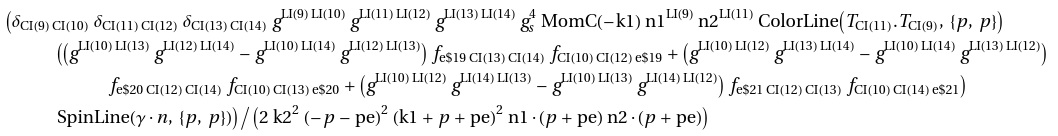
\includegraphics[width=\linewidth]{image7.png}
%	\caption{}
%	\label{fig:image7}
%\end{figure}
\\which translates to
\begin{align}
	&g_s^4\delta(-k_1)\delta_{c13c14}g^{l13l14}n_1^{l10}n_1^{l12}t^{c10}t^{c12}\frac{\bar u(P)\slashed n u(P)}{2k_2^2(-p-p_e)^2(k_1+p+p_e)^2n_1\cdot(p+p_e)n_2\cdot(p+p_e)}
	\notag\\&\bqty{\pqty{g^{l10l13}g^{l12l14}-g^{l10l14}g^{l12l13}}f^{e19c13c14}f^{c10c12e19}+\pqty{g^{l10l12}g^{l13l14}-g^{l10l14}g^{l13l12}}f^{e20c12c14}f^{c10c13e20}\notag\\&+\pqty{g^{l10l12}g^{l14l13}-g^{l10l13}g^{l14l12}}f^{e21c12c13}f^{c10c14e21}}\big|_{p_e=-x P^z\to -p,p=P,n\to z,k_2=l_2,n_1=n_2=n}
\end{align}
Taking $k_1=p+p_e-l_1$, the first line (that's excluding the four-gluon vertex) becomes
\begin{align}
	&g_s^4\delta(-k_1)\delta_{c13c14}g^{l13l14}n_1^{l10}n_1^{l12}t^{c10}t^{c12}\frac{\bar u(P)\slashed n u(P)}{2k_2^2(-p-p_e)^2(k_1+p+p_e)^2n_1\cdot(p+p_e)n_2\cdot(p+p_e)}\\
	=&g_s^4\delta(l_1-p-p_e)\delta_{c13c14}g^{l13l14}n_1^{l10}n_1^{l12}t^{c10}t^{c12}\frac{\bar u(P)\slashed n u(P)}{2l_2^2(-p-p_e)^2(2p+2p_e-l_1)^2n_1\cdot(p+p_e)n_2\cdot(p+p_e)}\\
	=&g_s^4\delta(l_1-p-p_e)\delta_{c13c14}g^{l13l14}n_1^{l10}n_1^{l12}t^{c10}t^{c12}\frac{\bar u(P)\slashed n u(P)}{2l_2^2l_1^2l_1^2n_1\cdot l_1n_2\cdot l_1}
\end{align}

Diagram~\ref{re:143} gives
\begin{align}
	&\frac{-ig_s^4}{2}\bar u(P)\slashed n u(P)
	\int\mm{l_1}\mm{l_2}n_{\tau}t^i\tilde D_G^{\tau\mu,ia}(l_1)\tilde D_G^{\sigma\lambda,dj}(l_1)\tilde D_G^{\nu\rho,bc}(l_2)n_{\lambda}t^j\frac{i}{n\cdot l_1+i\epsilon}\frac{i}{-n\cdot l_1+i\epsilon}\delta(l_1^z-(1-x)P^z) \notag\\&\left[f^{a b e} f^{c d e}\left(g^{\mu \rho} g^{\nu \sigma}-g^{\mu \sigma} g^{\nu \rho}\right)  +f^{a c e} f^{b d e}\left(g^{\mu \nu} g^{\rho \sigma}-g^{\mu \sigma} g^{\nu \rho}\right) +f^{a d e} f^{b c e}\left(g^{\mu \nu} g^{\rho \sigma}-g^{\mu \rho} g^{\nu \sigma}\right)\right]\\
	=&\frac{\overbrace{(-1)^3i^6}^{1}g_s^4}{2}\bar u(P)\slashed n u(P)
	\int\mm{l_1}\mm{l_2}\frac{n^{\mu}n^{\sigma}g^{\nu\rho}t^i\delta^{ia}t^j\delta^{dj}}{\bqty{l_1^2}^2\bqty{l_2^2}\bqty{n\cdot l_1}^2}\delta(l_1^z-(1-x)P^z) \notag\\&\left[f^{a b e} f^{c d e}\left(g^{\mu \rho} g^{\nu \sigma}-g^{\mu \sigma} g^{\nu \rho}\right)  +f^{a c e} f^{b d e}\left(g^{\mu \nu} g^{\rho \sigma}-g^{\mu \sigma} g^{\nu \rho}\right) +f^{a d e} f^{b c e}\left(g^{\mu \nu} g^{\rho \sigma}-g^{\mu \rho} g^{\nu \sigma}\right)\right]
\end{align}
Let's compare the color indices: 
\subsection{Numerical test (massless, ordered as Figure~\ref{re:sc} and Figure~\ref{re:c}, $z=1/4$)}
\subsubsection{Self-conjugated}
\paragraph{10}
\begin{minted}[breaklines]{mathematica}
	-((0.2026423672846755428877589264194553167160520680(3)*10^1)/ep)-0.13142890977(7)*10^2
\end{minted}
\paragraph{11}
\begin{minted}[breaklines]{mathematica}
	-((0.3609567167(4))/ep^2)-(0.16328193(1)*10^1)/ep-0.6455896(1)*10^1
\end{minted}
\paragraph{\textcolor{red}{11 xiong}	\WNNH}

\paragraph{26}
\begin{minted}[breaklines]{mathematica}
	-0.4052847345693513
\end{minted}
\paragraph{\textcolor{red}{26 xiong}}
\begin{minted}[breaklines]{mathematica}
	-0.405285
\end{minted}
\paragraph{27}
\begin{minted}[breaklines]{mathematica}
	-((0.1899772193(3)*10^-1)/ep^2)+(0.871746(1)*10^-2)/ep-0.4783185(9)*10^-1
\end{minted}
\paragraph{\textcolor{red}{27 xiong}}

\paragraph{52}
\begin{minted}[breaklines,breakbefore=-]{mathematica}
	(0.2251581858718617143197321404660614630178356311(1)*10^-1)/ep^3+(0.302543(3)*10^-2)/ep^2-(0.947637(3)*10^-1)/ep-0.692705(2)-I 0.0(1)*10^-5
\end{minted}
\paragraph{71}
\begin{minted}[breaklines,breakbefore=-/*]{mathematica}
	-((0.4052847345693510857755178528389106334321041360(3))/ep^2)-(0.19519788014(4)*10^1)/ep-0.823627359(1)*10^1
\end{minted}
\paragraph{\textcolor{red}{71 xiong}}

\paragraph{87}
\begin{minted}[breaklines]{mathematica}
	-((0.7205061947899574858231428494913966816570740196(4))/ep)-0.5969939054(1)*10^1
\end{minted}
\paragraph{\textcolor{red}{87 xiong}}

\paragraph{100}
\begin{minted}[breaklines]{mathematica}
	-0.1801265486974893714557857123728491704142685049(1)
\end{minted}
\paragraph{116}
\begin{minted}[breaklines]{mathematica}
	(0.6291855(4)*10^-1)/ep^2-(0.5159034(4))/ep-0.1258567(2)*10^1
\end{minted}
\paragraph{\textcolor{red}{116 xiong}	\WNZF AutoEnd Failed @ ALL possible bisections!}

\paragraph{124}
\begin{minted}[breaklines]{mathematica}
	(0.2701898230462340571836785685592737556214027573(3))/ep+0.16983474990(6)*10^1
\end{minted}
\paragraph{\textcolor{red}{124 xiong}}

\paragraph{125}
\begin{minted}[breaklines]{mathematica}
	(0.5066059182(3)*10^-1)/ep^2+(0.19628268(1))/ep+0.76838637(9)
\end{minted}
\paragraph{\textcolor{red}{125 xiong} \WNNH}
\paragraph{128}
\begin{minted}[breaklines]{mathematica}
	(0.7100744(2))/ep+0.1478379(1)*10^1
\end{minted}
\paragraph{\textcolor{red}{128	xiong}}

\paragraph{129}
\begin{minted}[breaklines]{mathematica}
	-((0.2725043(8)*10^-1)/ep^2)-(0.1354903(1))/ep+0.265727(5)*10^-1
\end{minted}
\paragraph{\textcolor{red}{129 xiong}}

\paragraph{133}
\begin{minted}[breaklines]{mathematica}
	(0.2880197(3)*10^-1)/ep^2-(0.1100423(3))/ep+0.1811499(1)*10^1
\end{minted}
\paragraph{\textcolor{red}{133	xiong} AutoEnd Failed @ ALL possible bisections!}

\paragraph{143}
\begin{minted}[breaklines]{mathematica}
	0
\end{minted}
\paragraph{\textcolor{red}{143 xiong}}

\paragraph{144}
\begin{minted}[breaklines]{mathematica}
	0
\end{minted}
\subsubsection{Remaining diagrams}
\paragraph{2	\WNNH}

\subparagraph{\CJ{1}	\WNNH}

\paragraph{3}

\subparagraph{\CJ{83}	\WNNH}
\paragraph{85	\WNNH}
\subparagraph{\CJ{4}}

\paragraph{5	\WNZF}
\subparagraph{\CJ{113}	\WNZF}
\paragraph{7}
\begin{minted}[breaklines]{mathematica}
	0
\end{minted}
\subparagraph{\CJ{6}}
\begin{minted}[breaklines]{mathematica}
	0
\end{minted}
\paragraph{13}
\begin{minted}[breaklines]{mathematica}
	(0.16042520743(9))/ep^2-(0.24060641(3))/ep-0.5034791(3)
\end{minted}
\subparagraph{\CJ{14}}
\begin{minted}[breaklines]{mathematica}
	(0.16042520743(9))/ep^2-(0.24060641(3))/ep-0.5034791(3)
\end{minted}
\paragraph{16}
\begin{minted}[breaklines]{mathematica}
	(0.72172896(3)*10^-1)/ep^2+(0.13916914(8))/ep+0.10188133(7)*10^1
\end{minted}
\subparagraph{\CJ{18}}
\begin{minted}[breaklines]{mathematica}
	(0.72172896(3)*10^-1)/ep^2+(0.13916914(8))/ep+0.10188133(7)*10^1
\end{minted}
\paragraph{25}
\begin{minted}[breaklines]{mathematica}
	(0.8443431970(5)*10^-2)/ep^2+(0.99323076(2)*10^-1)/ep+0.32267783(2)
\end{minted}
\subparagraph{\CJ{22}}
\begin{minted}[breaklines]{mathematica}
	(0.8443431970(5)*10^-2)/ep^2+(0.99323076(2)*10^-1)/ep+0.32267783(2)
\end{minted}
\paragraph{88}
\begin{minted}[breaklines]{mathematica}
	-((0.30021091(3)*10^-1)/ep^3)+(0.11491921(3)+I 0.18862808(2))/ep^2+(0.1510373(2)*10^1+I 0.13143394(4)*10^1)/ep+I 0.669150(1)*10^1+0.1158914(9)*10^2
\end{minted}
\subparagraph{\CJ{30}}
\begin{minted}[breaklines]{mathematica}
	-((0.300210915(7)*10^-1)/ep^3)+(-0.11023898(3)-I 0.18862808(1))/ep^2+(-0.5735834(7)-I 0.13143394(4)*10^1)/ep-0.227073(4)*10^1-I 0.6691519(9)*10^1
\end{minted}
\paragraph{31	\WNOF}

\subparagraph{\CJ{106}	\WNNH	\WNGINAC}
\subparagraph{\ZR{3.11}}
\paragraph{32	\WNOF}

\subparagraph{\CJ{82}	\WNNH}
\subparagraph{\ZR{3.12}}
\paragraph{38}
\begin{minted}[breaklines]{mathematica}
	-((0.4503163717437234286394642809321229260356712622(3)*10^-1)/ep^2)+(-0.26393587(2)+I 0.14147106(4))/ep-0.6590036(3)+I 0.6663843(5)
\end{minted}
\subparagraph{\CJ{62}}
\begin{minted}[breaklines]{mathematica}
	-((0.4503163717437234286394642809321229260356712622(3)*10^-1)/ep^2)+(-0.26393587(2)-I 0.14147106(1))/ep-0.65900358(7)-I 0.6663842(5)
\end{minted}
\paragraph{89 (3MIs)}
\begin{minted}[breaklines,breakbefore=-+]{mathematica}
	(0.1801265486974893714557857123728491704142685049(1))/ep^2+(0.6273774024(2))/ep+0.2771696389(5)*10^1
\end{minted}
\subparagraph{\CJ{39} (2MIs)}
\begin{minted}[breaklines,breakbefore=-+]{mathematica}
	(0.1801265486974893714557857123728491704142685049(1))/ep^2+(0.6273774024(2))/ep+0.2771696389(5)*10^1
\end{minted}
\paragraph{40}
\begin{minted}[breaklines]{mathematica}
	-((0.558142 - 0.565884 I)/ep) - (3.52786 - 2.48104 I)
\end{minted}
\subparagraph{\CJ{97}}
\begin{minted}[breaklines]{mathematica}
	(-0.5581423(1)-I 0.565884242(3))/ep-I 0.24810455(5)*10^1-0.3527861(1)*10^1
\end{minted}
\subparagraph{\ZR{3.15}}
\begin{minted}[breaklines]{mathematica}
	-(0.360253/ep)
\end{minted}
\paragraph{74	\WNZF}
\subparagraph{\CJ{41}	\WNGINAC	\WNDZ}
\paragraph{54}
\begin{minted}[breaklines]{mathematica}
	-((0.72050619478996(4))/ep)-I 0.226353697(2)*10^1-0.45289267(6)*10^1
\end{minted}
\subparagraph{\CJ{80}}
\begin{minted}[breaklines]{mathematica}
	-((0.720506194789957(2))/ep)+I 0.2263536968(3)*10^1-0.45289267(5)*10^1
\end{minted}
\subparagraph{\ZR{4.6}}
\paragraph{81}
\begin{minted}[breaklines]{mathematica}
	(0.1801265486974894(3))/ep^2+(0.78974126(8)-I 0.56588424(2))/ep+0.2441972(1)*10^1-I 0.24810455(7)*10^1
\end{minted}
\subparagraph{\CJ{55}}
\begin{minted}[breaklines]{mathematica}
	(0.18012654869749(3))/ep^2+(0.78974126(9)+I 0.565884242(4))/ep+0.24419718(8)*10^1+I 0.24810453(5)*10^1
\end{minted}
\subparagraph{\ZR{3.14}}

\paragraph{84}
\begin{minted}[breaklines]{mathematica}
	(0.1395356(1)+I 0.1414710(2))/ep^2+(0.6166541(5)+I 0.3512700(5))/ep+I 0.1219312(2)*10^1+0.1898527(2)*10^1
\end{minted}
\subparagraph{\CJ{56}}
\begin{minted}[breaklines]{mathematica}
	(0.1395356(2)-I 0.1414711(2))/ep^2+(0.6166541(7)-I 0.3512700(8))/ep-I 0.1219311(2)*10^1+0.1898527(2)*10^1
\end{minted}
\subparagraph{\ZR{4.2}}
\paragraph{86}
\begin{minted}[breaklines]{mathematica}
	-((0.900632743487447(2)*10^-1)/ep)+I 0.2829421211(4)-0.5661159(5)
\end{minted}
\subparagraph{\CJ{58}}
\begin{minted}[breaklines]{mathematica}
	-((0.90063274348745(5)*10^-1)/ep)-I 0.282942121(3)-0.56611583(7)
\end{minted}
\paragraph{95}
\begin{minted}[breaklines]{mathematica}
	(0.2251581858718617(4)*10^-1)/ep^2+(0.9871766(7)*10^-1-I 0.70735530(2)*10^-1)/ep+0.305247(1)-I 0.3101307(3)
\end{minted}
\subparagraph{\CJ{59}}
\begin{minted}[breaklines]{mathematica}
	(0.22515818587186(3)*10^-1)/ep^2+(0.9871766(1)*10^-1+I 0.707355303(5)*10^-1)/ep+0.3052465(1)+I 0.31013067(6)
\end{minted}
\paragraph{60}
\begin{minted}[breaklines]{mathematica}
	(0.45031637(2)*10^-1)/ep^2+(0.14234890(2)-I 0.70735530(8)*10^-1)/ep+0.2902786(2)-I 0.3562536(3)
\end{minted}
\subparagraph{\CJ{63}}
\begin{minted}[breaklines]{mathematica}
	(0.4503163717437(1)*10^-1)/ep^2+(0.14234890(7)+I 0.70735530(2)*10^-1)/ep+0.2902786(8)+I 0.3562535(2)
\end{minted}
\paragraph{61}
\begin{minted}[breaklines]{mathematica}
	-((0.11257909294(3)*10^-1)/ep^3)+(-0.141816(2)*10^-1+I 0.176839(2)*10^-1)/ep^2+(-0.61242(7)*10^-2+I 0.554395(8)*10^-1)/ep+0.120741(2)+I 0.225341(2)
\end{minted}
\subparagraph{\CJ{101}}
\begin{minted}[breaklines]{mathematica}
	-((0.11257909293593(2)*10^-1)/ep^3)+(-0.1418158(7)*10^-1-I 0.176838826(4)*10^-1)/ep^2+(-0.61242(3)*10^-2-I 0.5543947(5)*10^-1)/ep+0.120741(1)-I 0.2253407(6)
\end{minted}
\paragraph{64}
\begin{minted}[breaklines]{mathematica}
	(0.675474558(3)*10^-1)/ep^3+(0.55505288(5)-I 0.42441318(2))/ep^2+(0.24553798(8)*10^1-I 0.31694700(3)*10^1)/ep+0.5380347(5)*10^1-I 0.17422348(5)*10^2
\end{minted}
\subparagraph{\CJ{104}}
\begin{minted}[breaklines]{mathematica}
	(0.675474558(2)*10^-1)/ep^3+(0.48750543(5)+I 0.42441318(1))/ep^2+(0.19366015(6)*10^1+I 0.31694701(3)*10^1)/ep+0.2877105(4)*10^1+I 0.17422349(4)*10^2
\end{minted}
\paragraph{136}

\subparagraph{\CJ{102}	\WNNH}
\paragraph{103}
\begin{minted}[breaklines]{mathematica}
	(0.750527286(1)*10^-2)/ep^3+(0.13063137(6)*10^-1-I 0.1178926(2)*10^-1)/ep^2+(-0.281112(5)*10^-1+I 0.376194(2)*10^-1)/ep+I 0.243805(2)-0.58512(3)*10^-1
\end{minted}
\subparagraph{\CJ{108}}
\begin{minted}[breaklines]{mathematica}
	(0.7505272862(2)*10^-2)/ep^3+(0.13063137(6)*10^-1+I 0.1178926(2)*10^-1)/ep^2+(-0.281109(4)*10^-1-I 0.376194(2)*10^-1)/ep-I 0.243805(3)-0.58513(2)*10^-1
\end{minted}
\paragraph{127}
\begin{minted}[breaklines]{mathematica}
	-((0.7505272862(2)*10^-2)/ep^3)+(-0.3668912(2)*10^-1+I 0.1178926(4)*10^-1)/ep^2+(-0.1256239(4)-I 0.376194(2)*10^-1)/ep-I 0.24381(1)-0.617659(3)
\end{minted}
\subparagraph{\CJ{105}}
\begin{minted}[breaklines]{mathematica}
	-((0.7505272862(1)*10^-2)/ep^3)+(-0.20284742(6)*10^-1-I 0.1178926(2)*10^-1)/ep^2+(0.569092(5)*10^-1+I 0.1103759(2))/ep+0.312777(2)+I 0.679341(2)
\end{minted}
\paragraph{131}
\begin{minted}[breaklines]{mathematica}
	-((0.21235731(2)*10^-1)/ep^2)-(0.7878081(2)*10^-1)/ep-0.4849994(2)
\end{minted}
\subparagraph{\CJ{110}}
\begin{minted}[breaklines]{mathematica}
	-((0.21235731(2)*10^-1)/ep^2)-(0.7878081(2)*10^-1)/ep-0.4849994(1)
\end{minted}
\paragraph{121}
\begin{minted}[breaklines]{mathematica}
	-((0.4503163717(1)*10^-1)/ep^2)-(0.143889556(4))/ep-0.9841648(2)
\end{minted}
\subparagraph{\CJ{111}}
\begin{minted}[breaklines]{mathematica}
	-((0.4503163717(1)*10^-1)/ep^2)-(0.143889556(4))/ep-0.9841648(2)
\end{minted}
\paragraph{126}
\begin{minted}[breaklines]{mathematica}
	(0.10132118364(2))/ep^2+(0.154882861(5))/ep+0.8068632(2)
\end{minted}
\subparagraph{\CJ{117}}
\begin{minted}[breaklines]{mathematica}
	(0.10132118364(2))/ep^2+(0.154882861(5))/ep+0.8068632(2)
\end{minted}
\paragraph{123}
\begin{minted}[breaklines]{mathematica}
	-((0.2251581859(1)*10^-1)/ep^2)+(0.27844106(4)*10^-1)/ep+0.2197552(4)*10^-1
\end{minted}
\subparagraph{\CJ{119}}
\begin{minted}[breaklines]{mathematica}
	-((0.2251581859(1)*10^-1)/ep^2)+(0.27844106(4)*10^-1)/ep+0.2197552(4)*10^-1
\end{minted}
\paragraph{135}
\begin{minted}[breaklines]{mathematica}
	(0.8824885(6)*10^-2)/ep^2-(0.4259655(6)*10^-1)/ep-0.1357314(2)
\end{minted}
\subparagraph{\CJ{134}}
\begin{minted}[breaklines]{mathematica}
	(0.8824885(5)*10^-2)/ep^2-(0.4259655(5)*10^-1)/ep-0.1357314(2)
\end{minted}
\subparagraph{\ZR{3.4}}
\paragraph{142}
\begin{minted}[breaklines]{mathematica}
	0
\end{minted}
\subparagraph{\CJ{139}}
\begin{minted}[breaklines]{mathematica}
	0
\end{minted}
\subsection{Numerical test (ordered as Figure~\ref{re:sc} and Figure~\ref{re:c}, $z=1/4$)}
\subsubsection{Self-conjugated}
\paragraph{10}
\begin{minted}[breaklines]{mathematica}
	-13.142892209573214 - 2.0264236728467586/ep
\end{minted}
\paragraph{11}
\begin{minted}[breaklines]{mathematica}
	(-0.721913433451656621537641175369309494168040468603083244938 log(s)-0.214490046(8))/ep+0.721913433451656621537641175369309494168040468603083244938 log^2(s)-0.2836658516(3)*10^1 log(s)-0.327680(1)*10^1
\end{minted}
\paragraph{\textcolor{red}{11 xiong}	\WNNH}
\begin{minted}[breaklines]{mathematica}
	968.417+24.7655/ep
\end{minted}
\paragraph{26}
\begin{minted}[breaklines]{mathematica}
	-0.4052847345693513
\end{minted}
\paragraph{\textcolor{red}{26 xiong}}
\begin{minted}[breaklines]{mathematica}
	-0.405285
\end{minted}
\paragraph{27}
\begin{minted}[breaklines]{mathematica}
	(0.95364928(1)*10^-1-0.0379954438658766642914547987036478574722246996482761990896 log(s))/ep+0.0379954438658766642914547987036478574722246996482761990896 log^2(s)-0.1732949391(5) log(s)+0.174213(4)
\end{minted}
\paragraph{\textcolor{red}{27 xiong}}
\begin{minted}[breaklines]{mathematica}
	50.484+1.38493/ep
\end{minted}
\paragraph{52	\WNNH}
\begin{minted}[breaklines]{c}
	NAN=198 v.s. RUN=99
	NAN=198 v.s. RUN=99
	NAN=198 v.s. RUN=99
	NAN=198 v.s. RUN=99
	NAN=198 v.s. RUN=99
	NAN=198 v.s. RUN=99
	NAN=198 v.s. RUN=99
	NAN=198 v.s. RUN=99
	smin = -1, optimized lambda NOT found!
	JPCquasiR: SD.cpp:3732: void HepLib::SD::Integrates(const char*, const char*, int): Assertion `false' failed.
\end{minted}
\paragraph{71}
\begin{minted}[breaklines]{mathematica}
	(0.40528473456935108577551785283891061393612511304014832705485 (-log(s))-0.423786494(1))/ep+0.20264236728467554288775892641945530696806255652007416352742 log^2(s)-0.1528192308(1)*10^1 log(s)-0.49684439(1)*10^1
\end{minted}
\paragraph{\textcolor{red}{71 xiong}}
\begin{minted}[breaklines]{mathematica}
(-0.405285 log(s)-0.423787)/ep+0.202642 log^2(s)-1.52819 log(s)-4.96844
\end{minted}
\paragraph{87}
\begin{minted}[breaklines]{mathematica}
	-((0.7205061947899575(4))/ep)-0.5969939(1)*10^1
\end{minted}
\paragraph{\textcolor{red}{87 xiong}}
\begin{minted}[breaklines]{mathematica}
-5.96994 - 0.720506/ep
\end{minted}
\paragraph{100}
\begin{minted}[breaklines]{mathematica}
	-0.1801265486974893714557859019664687608595103043616168293442
\end{minted}
\paragraph{116	\WNNH}
\begin{minted}[breaklines]{mathematica}
	Failed IDs: {12, 13, 20, 21, 22, }
\end{minted}
\paragraph{\textcolor{red}{116 xiong}	\WNZF AutoEnd Failed @ ALL possible bisections!}

\paragraph{124}
\begin{minted}[breaklines]{mathematica}
	(0.270190 CV(1,3))/ep+1.69835 CV(1,3)
\end{minted}
\paragraph{\textcolor{red}{124 xiong}}
\begin{minted}[breaklines]{mathematica}
(0.27019 CV(1,3))/ep+1.69835 CV(1,3)
\end{minted}
\paragraph{125	\WNNH}
\begin{minted}[breaklines]{mathematica}
	(CV(1,3) (0.101321 log(s)+0.0158833))/ep+0.151982 (-CV(1,3)) log^2(s)-I 0.318310 CV(1,3) log(s)+0.473347 CV(1,3) log(s)+(0.0(5)*10^-7 CV(1,3))/s+(I 0.3(3)*10^-7 CV(1,3))/s+I 0.48(4)*10^1 CV(1,3)+0.83(4)*10^1 CV(1,3)
\end{minted}
\paragraph{\textcolor{red}{125 xiong} \WNNH}
\paragraph{128}
\begin{minted}[breaklines]{mathematica}
	-((0.0(5)*10^-7 CV(1,3))/ep^2)+((0.81056947(3) CV(1,3))/s+0.0(4)*10^-7 CV(1,3) log(s)+0.2026424(3) CV(1,3))/ep+0.5074321(1) CV(1,3) log(s)-(0.810569 CV(1,3) log(s))/s+(0.45612729(2)*10^1 CV(1,3))/s+0.0(2)*10^-7 (-CV(1,3)) log^2(s)+0.13766891(1)*10^2 CV(1,3)
\end{minted}
\paragraph{\textcolor{red}{128	xiong}}
\begin{minted}[breaklines]{mathematica}
	((0.810569 CV(1,3))/s+0.202642 CV(1,3))/ep+(4.56127 CV(1,3))/s-(0.810569 CV(1,3) log(s))/s+0.507432 CV(1,3) log(s)+13.7669 CV(1,3)
\end{minted}
\paragraph{129	\WNNH}
\begin{minted}[breaklines]{mathematica}
	((0.500352 CV(1,3))/s+0.500352 CV(1,3)+(0.0180127 -2.54985*10^-8 I)/s-(9.42776*10^-8+7.15663*10^-8 I))/ep+(2.78522 CV(1,3))/s-(0.500352 CV(1,3) log(s))/s-0.500352 CV(1,3) log(s)+2.78522 CV(1,3)+(0.526293 -0.0565893 I)/s+(0.0725309 -4.81307*10^-8 I) log(s)+(0.253132 -0.452708 I)+(0.148304 log(s))/s
\end{minted}
\paragraph{\textcolor{red}{129 xiong}}
\begin{minted}[breaklines]{mathematica}
((0.810569 CV(1,3))/s+0.202642 CV(1,3))/ep+(4.56127 CV(1,3))/s-(0.810569 CV(1,3) log(s))/s+0.507432 CV(1,3) log(s)+13.7669 CV(1,3)
\end{minted}
\paragraph{133	\WNNH}
\begin{minted}[breaklines]{c}
	AutoEnd Failed @ ALL possible bisections!
	JPCquasiR: SD.cpp:138: std::vector<std::pair<GiNaC::container<std::list>, GiNaC::container<std::list> > > HepLib::SD::AutoEnd(std::pair<GiNaC::container<std::list>, GiNaC::container<std::list> >): Assertion `false' failed.
\end{minted}
\paragraph{\textcolor{red}{133	xiong} AutoEnd Failed @ ALL possible bisections!}

\paragraph{143}
\begin{minted}[breaklines]{mathematica}
	0
\end{minted}
\paragraph{\textcolor{red}{143 xiong}}
\begin{minted}[breaklines]{mathematica}
AutoEnd Failed @ ALL possible bisections!
\end{minted}
\paragraph{144}
\begin{minted}[breaklines]{mathematica}
	0
\end{minted}
\subsubsection{Remaining diagrams}
\paragraph{2}
\begin{minted}[breaklines]{mathematica}
	
\end{minted}
\subparagraph{\CJ{1}	\WNNH}
\begin{minted}[breaklines]{mathematica}
	-((0.455945 log(s)+0.2886892(1)+I 0.143239449(8)*10^1)/ep^2)-(0.227973 (-s) log^2(s)+s (0.0(1)*10^6-I 0.3(3)*10^6)+(1.21585+s (0.424773500(9)*10^1+I 0.15915495(6))) log(s)+0.0(1)*10^6-I 0.3(2)*10^6)/(ep s)-(3.64756 log(s))/s^2-(0.0(4)*10^6)/s^2+(I 1.0(7)*10^6)/s^2-0.0759909 log^3(s)+(0.607927 log^2(s))/s-(22.2444 log(s))/s+(0.0(2)*10^7)/s+(I 0.2(4)*10^7)/s+I 0.7957747(3)*10^-1 log^2(s)+0.212386750(4)*10^1 log^2(s)-I 0.13271482(2)*10^1 log(s)-0.214233808(5)*10^2 log(s)+0.1(2)*10^7+I 0.3(4)*10^7
\end{minted}
\paragraph{3}
\begin{minted}[breaklines]{mathematica}
	-((2.67042 +2.12028 I)/s^2)-((0.260912 -1.01859 I) log(s))/s^2+(14.6734 +1.31932 I)/s-((0.324228 +3.72868*10^-9 I) log^2(s))/s+(0.222907 -5.53015*10^-9 I) log^2(s)+((0.881442 -3.43775 I) log(s))/s+(0.673891 -1.68704 I) log(s)+(13.4354 -26.5232 I)+(-((4.70467*10^-9+1.04672*10^-9 I)/s^2)-(1.49279*10^-8+4.88207*10^-9 I)/s+(-3.02109*10^-8-6.73934*10^-9 I))/ep^2+(1/ep)(-((2.61261*10^-8+1.68009*10^-8 I)/s^2)-((4.70467*10^-9+1.04672*10^-9 I) log(s))/s^2-(1.30934*10^-7+9.62535*10^-8 I)/s-((1.49279*10^-8+4.88207*10^-9 I) log(s))/s-(3.02109*10^-8+6.73934*10^-9 I) log(s)-(3.63837*10^-7+2.4728*10^-7 I))-((3.64128*10^-9+8.50597*10^-10 I) log^2(s))/s^2
\end{minted}
\subparagraph{\CJ{83}	\WNNH}
\paragraph{85	\WNNH}
\subparagraph{\CJ{4}}
\begin{minted}[breaklines]{mathematica}
	-((2.42703 -0.625114 I)/s)+((0.0810569 -3.18897*10^-9 I) log^2(s))/s-(0.0405285 +2.8617*10^-9 I) log^2(s)+((0.0994902 +1.01859 I) log(s))/s+(0.0313118 -0.509296 I) log(s)+(1.1822 +0.196737 I)+((-5.16401*10^-10-3.70072*10^-9 I)-(5.50793*10^-10+3.94743*10^-9 I)/s)/ep^2+(-((2.78596*10^-8+7.69087*10^-8 I)/s)-((5.50793*10^-10+3.94743*10^-9 I) log(s))/s-(5.16401*10^-10+3.70072*10^-9 I) log(s)-(3.69889*10^-8+6.98559*10^-8 I))/ep
\end{minted}
\paragraph{5}
\begin{minted}[breaklines]{mathematica}
	(-((0.3419589947928899786230931883328307387152218491(3))/s)-0.12918450914(7)*10^1)/ep^2+(1/ep)(-((0.10258769843786699358692795649984922168734618543(9)*10^1)/s^2)-0.11398633159762999287436439611094361761455281466(3) log^2(s)+(0.34195899479288997862309318833283074349804313682(7) log(s))/s-(0.8382561761(1)*10^1)/s+0.12918450914(6)*10^1 log(s)-0.1470414820(6)*10^2)-(0.3077630953136009807607838694995476650620431481(3)*10^1)/s^3-(0.35406455127(4)*10^2)/s^2+(0.10258769843786699358692795649984922305000068822(2)*10^1 log(s))/s^2+0.11398633159762999287436439611094360171680492877(1) log^3(s)-(0.51293849218933496793463978249924613414931972596(7) log^2(s))/s-(0.132919978(2)*10^3)/s-0.19124846658(3)*10^1 log^2(s)+(0.104343157298(2)*10^2 log(s))/s+0.2985081056(3)*10^2 log(s)-0.17571608(1)*10^3
\end{minted}
\subparagraph{\CJ{113}}
\begin{minted}[breaklines]{mathematica}
	(-((0.3419589947928899786230931883328307373430847421(3))/s)-0.14184965710(7)*10^1)/ep^2+(1/ep)(-((0.10258769843786699358692795649984922122454579432(9)*10^1)/s^2)-0.11398633159762999287436439611094358537143515056(3) log^2(s)+(0.34195899479288997862309318833283073307983918224(6) log(s))/s-(0.99213772376(4)*10^1)/s+0.14184965710(6)*10^1 log(s)-0.1937716819(6)*10^2)-(0.3077630953136009807607838694995476636730496358(3)*10^1)/s^3-(0.40022901557(1)*10^2)/s^2+(0.10258769843786699358692795649984921992453950185(2)*10^1 log(s))/s^2+0.11398633159762999287436439611094359096909904074(1) log^3(s)-(0.51293849218933496793463978249924612373111577138(6) log^2(s))/s-(0.166808716(2)*10^3)/s-0.24887488978(3)*10^1 log^2(s)+(0.119731312064(2)*10^2 log(s))/s+0.3760146151(3)*10^2 log(s)-0.22781445(1)*10^3
\end{minted}
\paragraph{7}
\begin{minted}[breaklines]{mathematica}
	0
\end{minted}
\subparagraph{\CJ{6}}
\begin{minted}[breaklines]{mathematica}
	0
\end{minted}
\subparagraph{\ZR{4.9}}
\begin{minted}[breaklines]{mathematica}
	0
\end{minted}
\paragraph{13	\WNZF}
\subparagraph{\CJ{14}}
\begin{minted}[breaklines]{mathematica}
	(0.108076/s^2-0.770041/s)/ep+1.09363/s^2-6.67758/s-1.08404*10^-6
\end{minted}
\paragraph{16}
\begin{minted}[breaklines]{mathematica}
	-((0.211474 +1.27324 I)/s^2)+(2.28897 -1.08225 I)/s-(4.7286 -0.668451 I)+(-(6.7167*10^-16/s^2)+0.486342/s-0.729513)/ep-(3.00378*10^-16 log(s))/s^2-(0.486342 log(s))/s+0.729513 log(s)
\end{minted}
\subparagraph{\CJ{18}	\WNZF}
\paragraph{25	\WNZF}
\subparagraph{\CJ{22}}
\begin{minted}[breaklines]{mathematica}
	(0.0810569/s-0.054038/s^2)/ep-0.411721/s^2+0.617579/s
\end{minted}
\paragraph{88	\WNZF}
\subparagraph{\CJ{30}}
\begin{minted}[breaklines]{mathematica}
	-((0.394011 +1.25922*10^-8 I)/s)+(0.782248 -2.46415*10^-8 I)+(0.168118 log(s))/s-0.354249 log(s)
\end{minted}
\paragraph{31	\WNOF}
\begin{minted}[breaklines]{mathematica}
	-((0.162114 +1.91875*10^-8 I)/ep^3)+(-0.324228 log(s)-(92.0766 +2.65448 I))/ep^2+1/ep (-((158.541 +3.48593 I)/s)+(32.6052 +0.63662 I) log(s)-0.0405285 log^2(s)-(1.58061 log(s))/s-(1.91238*10^10+1.98727*10^10 I))-(475.619 +10.4578 I)/s^2-(12502.7 +1351.46 I)/s-(16.9633 +0.31831 I) log^2(s)-(4.74183 log(s))/s^2+0.148604 log^3(s)+(0.790305 log^2(s))/s+(81.2751 log(s))/s+(4.05197*10^10-6.80923*10^10 I) log(s)+(6.59315*10^13-1.55809*10^14 I)
\end{minted}
\subparagraph{\CJ{106}	\WNNH	\WNGINAC}
\subparagraph{\ZR{3.11}}
\paragraph{32	\WNOF}
\begin{minted}[breaklines]{mathematica}
	-((0.162114 +1.91875*10^-8 I)/ep^3)+(-0.324228 log(s)-(92.0766 +2.65448 I))/ep^2+1/ep (-((158.541 +3.48593 I)/s)+(32.6052 +0.63662 I) log(s)-0.0405285 log^2(s)-(1.58061 log(s))/s-(1.91238*10^10+1.98727*10^10 I))-(475.619 +10.4578 I)/s^2-(12502.7 +1351.46 I)/s-(16.9633 +0.31831 I) log^2(s)-(4.74183 log(s))/s^2+0.148604 log^3(s)+(0.790305 log^2(s))/s+(81.2751 log(s))/s+(4.05197*10^10-6.80923*10^10 I) log(s)+(6.59315*10^13-1.55809*10^14 I)
\end{minted}
\subparagraph{\CJ{82}	\WNNH}
\subparagraph{\ZR{3.12}}
\paragraph{31+32}
\begin{minted}[breaklines]{mathematica}
	
\end{minted}
\paragraph{38	\WNZF}
\subparagraph{\CJ{62}	\WNZF}
\paragraph{89	\WNDIV}
\subparagraph{\CJ{39}	\WNDIV}
\paragraph{40}
\begin{minted}[breaklines]{mathematica}
	-((0.3602531(6))/ep)+0.1978893(4) (-log(s))+I 0.5658842(7) log(s)-I 0.72868(2)-0.170150(1)*10^1
\end{minted}
\subparagraph{\CJ{97}}
\begin{minted}[breaklines]{mathematica}
	-((0.3602531(4))/ep)+0.1978892(3) (-log(s))-I 0.5658841(5) log(s)+I 0.72868(1)-0.170150(1)*10^1
\end{minted}
\subparagraph{\ZR{3.15}}
\begin{minted}[breaklines]{mathematica}
	-(0.360253/ep)
\end{minted}
\paragraph{74	\WNZF}
\subparagraph{\CJ{41}	\WNGINAC	\WNDZ}
\paragraph{54}
\begin{minted}[breaklines]{mathematica}
	-((0.72050619478996(4))/ep)-I 0.226353697(2)*10^1-0.45289267(6)*10^1
\end{minted}
\subparagraph{\CJ{80}}
\begin{minted}[breaklines]{mathematica}
	-((0.720506194789957(2))/ep)+I 0.2263536968(3)*10^1-0.4528927(6)*10^1
\end{minted}
\subparagraph{\ZR{4.6}}
\begin{minted}[breaklines]{mathematica}
	-2*(0.720506/ep)
\end{minted}
\paragraph{81}
\begin{minted}[breaklines]{mathematica}
	((0.180127 -9.13154*10^-9 I) log(s)-(0.231946 +7.6754*10^-8 I))/ep+(1.02169 -0.565884 I) log(s)-(0.815813 -0.728676 I)-(5.2095*10^-10+1.21468*10^-8 I)/ep^2+(-0.0900633-4.02323*10^-9 I) log^2(s)
\end{minted}
\subparagraph{\CJ{55}}
\begin{minted}[breaklines]{mathematica}
	((0.288202 -2.40402*10^-8 I)/s-(0.432304 +3.26984*10^-8 I))/ep+(1.81157 +0.905414 I)/s-(2.71736 +1.35812 I)
\end{minted}
\subparagraph{\ZR{3.14}}
\begin{minted}[breaklines]{mathematica}
	2*(0.180127 log(s)-0.231946)/ep
\end{minted}
\paragraph{84}
\begin{minted}[breaklines]{mathematica}
	(-0.900633(1)*10^-1 log(s)-0.154217(3)-I 0.0(4)*10^-5)/ep+I 0.14147106(8) log^2(s)+0.27463050(8) log^2(s)-I 0.364339(2) log(s)-0.823115(2) log(s)+I 0.2156(8)-0.11134(8)*10^1
\end{minted}
\subparagraph{\CJ{56}}
\begin{minted}[breaklines]{mathematica}
	(-0.1125791(1) log(s)+I 0.0(3)*10^-5-0.80192(3)*10^-1)/ep-I 0.1414711(1) log^2(s)+0.2858884(1) log^2(s)+I 0.364340(2) log(s)-0.975562(2) log(s)-0.66278(3)-I 0.0(5)*10^10
\end{minted}
\subparagraph{\ZR{4.2}}
\begin{minted}[breaklines]{mathematica}
	2*(0.115973 -0.0900633 log(s))/ep
\end{minted}
\paragraph{86}
\begin{minted}[breaklines]{mathematica}
	-((0.900632743487447(2)*10^-1)/ep)+I 0.2829421211(4)-0.566116(6)
\end{minted}
\subparagraph{\CJ{58}}
\begin{minted}[breaklines]{mathematica}
	-((0.9006327434874(2)*10^-1)/ep)-I 0.282942121(3)-0.56611583(7)
\end{minted}
\subparagraph{\ZR{4.7}}
\begin{minted}[breaklines]{mathematica}
	-2*(0.0900633/ep)
\end{minted}
\paragraph{95}
\begin{minted}[breaklines]{mathematica}
	(0.225158185872(7)*10^-1 log(s)-0.289932(5)*10^-1)/ep+0.1277109(3) log(s)-0.112579092936(3)*10^-1 log^2(s)-I 0.707355(5)*10^-1 log(s)-0.10198(1)+I 0.9108(1)*10^-1
\end{minted}
\subparagraph{\CJ{59}}
\begin{minted}[breaklines]{mathematica}
	(0.22515818587186171431973214046606133(7)*10^-1 log(s)-0.289932(5)*10^-1)/ep+0.1277109(2) log(s)-0.11257909293593085715986607023303066(3)*10^-1 log^2(s)+I 0.707355(2)*10^-1 log(s)-0.101977(9)-I 0.9108(1)*10^-1
\end{minted}
\subparagraph{\ZR{4.1}}
\begin{minted}[breaklines]{mathematica}
	2*(0.0289932 -0.0225158 log(s))/ep
\end{minted}
\paragraph{60	\WNZF}
\subparagraph{\CJ{63}	\WNZF}
\paragraph{61}
\begin{minted}[breaklines]{mathematica}
	((0.0249708 +0.0565884 I)/s-(0.0409356 +0.113177 I)-(0.0180127 log(s))/s+0.0360253 log(s))/ep+(0.121805 +0.302986 I)/s-((0.0819104 +0.0282942 I) log(s))/s+(0.123545 +0.12025 I) log(s)-(0.132015 +0.412085 I)+((-1.70997*10^-8-7.51261*10^-9 I)-(3.80204*10^-10+2.72486*10^-9 I)/s)/ep^2-1.51762*10^-7/s^2+(0.00900633 log^2(s))/s-0.0180127 log^2(s)
\end{minted}
\subparagraph{\CJ{101}}
\begin{minted}[breaklines]{mathematica}
	((0. -5.44316*10^-9 I) log(s)-(5.06726*10^-8+1.09474*10^-7 I))/ep^2+((0.0301033 -0.0353678 I) log(s)-(0.0200969 -0.045542 I)-(1.32299*10^-8+4.49679*10^-9 I)/s+(-0.0112579-3.05202*10^-9 I) log^2(s))/ep+(0.0112579 -9.07187*10^-10 I) log^3(s)-(0.0593367 -0.0353677 I) log^2(s)+(0.0923378 -0.190433 I) log(s)-(0.0423955 -0.117755 I)-(1.47432*10^-10+8.25276*10^-9 I)/ep^3-(4.6093*10^-7+4.84678*10^-8 I)/s
\end{minted}
\paragraph{64	\WNZF}
\subparagraph{\CJ{104}	\WNZF}
\paragraph{136}
\begin{minted}[breaklines]{mathematica}
	(-((0.00499433 +0.0113178 I)/s)+(0.000695404 +0.00565863 I)+(0.00360253 log(s))/s-0.00180128 log(s))/ep+(0.232843 -0.0984924 I)/s+((0.0363448 +0.0226354 I) log(s))/s+(0.0153548 -1.05329*10^-7 I) log(s)-(0.653916 -3.42529 I)+((-1.16122*10^-8-2.31214*10^-9 I)-(4.75779*10^-9+2.54986*10^-9 I)/s)/ep^2-2.41702*10^-7/s^2-(0.0054038 log^2(s))/s+0.00270189 log^2(s)
\end{minted}
\subparagraph{\CJ{102}	\WNNH}
\paragraph{103	\WNZF}
\subparagraph{\CJ{108}	\WNZF}
\paragraph{127	\WNZF}
\subparagraph{\CJ{105}	\WNZF}
\paragraph{131}
\begin{minted}[breaklines]{mathematica}
	(0.027019 -0.0180127/s)/ep+0.0890396/s+(0.0180127 log(s))/s-0.027019 log(s)+0.197988
\end{minted}
\subparagraph{\CJ{110}	\WNZF}
\paragraph{121	\WNZF}
\subparagraph{\CJ{111}	\WNZF}
\paragraph{126}
\begin{minted}[breaklines]{mathematica}
	-(0.478416/(ep s))-3.57259/s+(0.478416 log(s))/s
\end{minted}
\subparagraph{\CJ{117}}
\begin{minted}[breaklines]{mathematica}
	(0.337737 log(s)+(12.5141 +0.065117 I))/ep+(4.9247 +0.043133 I)/s-(7.6631 +0.248286 I) log(s)+(960.52 -2.012 I)-0.371511 log^2(s)+(0.0506606 log(s))/s
\end{minted}
\paragraph{123	\WNZF}
\subparagraph{\CJ{119}}
\begin{minted}[breaklines]{mathematica}
	((0.108076 CV(1,3))/s-(0.0720506 CV(1,3))/s^2)/ep-(0.621011 CV(1,3))/s^2-(0.221294 CV(1,3))/s+0.51236 CV(1,3) log(s)+0.289007 CV(1,3)
\end{minted}
\paragraph{135}
\begin{minted}[breaklines,breakanywhere]{mathematica}
	-((0.75052728623953904773244046822021(1)*10^-2)/ep^2)+(-((0.2216400892176138750334863257712791698673512155(5)*10^-1)/s)+0.328355687729798333382942704846342(2)*10^-1 log(s)+0.1195769047(6))/ep-(0.6649202676528416251004589773138375479731914560(6)*10^-1)/s^2-(0.46125458376(8))/s-0.403111986217495687167289442761083(2)*10^-1 log^2(s)+(0.22164008921761387503348632577127917203974334809(4)*10^-1 log(s))/s-0.275899853(5)*10^-1 log(s)+0.935583(2)
\end{minted}
\subparagraph{\CJ{134}}
\begin{minted}[breaklines,breakanywhere]{mathematica}
	(0.93815910779942380966555(8)*10^-3)/ep^2+(-((0.1583143494(1)*10^-1)/s)+0.243921368027850190513043(1)*10^-1 log(s)+0.1710538662(7))/ep-(0.4749430483234583036431849837955982459939784269(4)*10^-1)/s^2-(0.321325679(2))/s-0.339786246441034580014865(1)*10^-1 log^2(s)+(0.15831434944(1)*10^-1 log(s))/s-0.917320947(5)*10^-1 log(s)+0.1254593(2)*10^1
\end{minted}
\paragraph{142}
\begin{minted}[breaklines]{mathematica}
	0
\end{minted}
\subparagraph{\CJ{139}}
\begin{minted}[breaklines]{mathematica}
	0
\end{minted}
% \subsection{A first attempt}
% Let's first take a look at the following diagram
% \begin{align}
% 	\begin{tikzpicture}[transform shape,scale=1.2,baseline=($(a)!0.5!(exa)$.base)]
% 		\begin{feynman}
% 			\node[dot] (a);
% 			\node[right=\FDWidth of a,dot] (b);
% 			\vertex at ($(a)!0.5!(b)$) (o);
% 			\vertex[below=\FDHeight of a] (exa);
% 			\vertex[below=\FDHeight of b] (exb);
% 			\vertex at ($(exa)!0.25!(a)$) (a1);
% 			\vertex at ($(exa)!0.75!(a)$) (a2);
% 			\vertex at ($(a1)!0.5!(a2)!1.2!-90:(a2)$) (g1);
% 			\vertex at ($(exb)!0.5!(b)$) (b1);
% 			\diagram*{
% 			(o) --[Eikonal,momentum=\(P-l_1-l_2\)] (b);
% 			(exa) --[fermion,momentum=\(P\)] (a1) --[fermion,momentum=\(l_1\)] (a2) --[fermion,momentum=\(l_1+l_2\)] (a);
% 			(a1) --[gluon,half right,looseness=2] (a2);
% 			(a1) --[quarter right,tikzmom'={0.2}{2mm}{-2pt}{$P-l_1$},draw=none] (g1) --[quarter right,tikzmom'={0.2}{2mm}{-2pt}{$l_2$},draw=none] (a2);
% 			(b) --[fermion,momentum=\(P\)] (exb);
% 			(g1) --[gluon,tikzmom'={0.2}{2mm}{-2pt}{$P-l_1-l_2$}] (o);
% 			};
% 		\end{feynman}
% 	\end{tikzpicture}
% \end{align}
% And

\clearpage
\section{Virtual Diagrams (Excluding Gauge Link Self-Energy Diagrams)}
\subsection{All diagrams}
\renewcommand*\thesubfigure{\roman{subfigure}}
\begin{figure}[!hbtp]
	\centering\hfil
	\subfloat[75]{
		\begin{tikzpicture}[transform shape,scale=1,baseline=($(a)!0.5!(exa)$.base)]
			\begin{feynman}
				\node[dot] (a);
				\node[right=\FDWidth of a,dot] (b);
				\vertex[below=\FDHeight of a] (exa);
				\vertex[below=\FDHeight of b] (exb);
				% 
				\vertex at ($(a)!0.33!(b)$) (o13);
				\vertex at ($(a)!0.66!(b)$) (o23);
				\vertex at ($(a)!0.25!(b)$) (o14);
				\vertex at ($(a)!0.5!(b)$) (o12);
				\vertex at ($(a)!0.75!(b)$) (o34);
				% 
				\vertex at ($(exa)!0.25!(a)$) (a14);
				\vertex at ($(exa)!0.5!(a)$) (a12);
				\vertex at ($(exa)!0.75!(a)$) (a34);
				% 
				\vertex at ($(exb)!0.25!(b)$) (b14);
				\vertex at ($(exb)!0.5!(b)$) (b12);
				\vertex at ($(exb)!0.75!(b)$) (b34);
				% 
				\vertex at ($(a12)!0.33!(b12)$) (ab13);
				\vertex at ($(a12)!0.66!(b12)$) (ab23);
				\vertex at ($(a12)!0.5!(b12)$) (ab12);
				% 
				\diagram*{
				(a) --[Eikonal] (o13);
				(o23) --[Eikonal] (b);
				(exa) --[fermion] (a12) --[fermion] (a);
				(b) --[fermion] (b12) --[fermion] (exb);
				(a12) --[gluon] (o13);
				(o23) --[gluon] (b12);
				};
			\end{feynman}
		\end{tikzpicture}
		\label{}
	}\hfil
	\caption{All self-conjugated virtual diagrams (actually there's only one). }
	\label{vir:sc}
\end{figure}
\begin{figure}[!hbtp]
	\centering\hfil
	\subfloat[8\red{/2.9}]{
		\begin{tikzpicture}[transform shape,scale=1,baseline=($(a)!0.5!(exa)$.base)]
			\begin{feynman}
				\node[dot] (a);
				\node[right=\FDWidth of a,dot] (b);
				\vertex[below=\FDHeight of a] (exa);
				\vertex[below=\FDHeight of b] (exb);
				% 
				\vertex at ($(a)!0.33!(b)$) (o13);
				\vertex at ($(a)!0.66!(b)$) (o23);
				\vertex at ($(a)!0.25!(b)$) (o14);
				\vertex at ($(a)!0.5!(b)$) (o12);
				\vertex at ($(a)!0.75!(b)$) (o34);
				% 
				\vertex at ($(exa)!0.25!(a)$) (a14);
				\vertex at ($(exa)!0.5!(a)$) (a12);
				\vertex at ($(exa)!0.75!(a)$) (a34);
				% 
				\vertex at ($(exb)!0.25!(b)$) (b14);
				\vertex at ($(exb)!0.5!(b)$) (b12);
				\vertex at ($(exb)!0.75!(b)$) (b34);
				% 
				\vertex at ($(a12)!0.33!(b12)$) (ab13);
				\vertex at ($(a12)!0.66!(b12)$) (ab23);
				\vertex at ($(a12)!0.5!(b12)$) (ab12);
				% 
				\vertex at ($(a14)!0.5!(a34)!1.2!-90:(a34)$) (g1);
				\vertex at ($(o12)!0.66!(a12)$) (g13);
				\vertex at ($(o12)!0.33!(a12)$) (g23);
				% 
				\diagram*{
				(a) --[Eikonal] (o12);
				(exa) --[fermion] (a12) --[fermion] (a);
				(b) --[fermion] (exb);
				(a12) --[gluon] (g13);
				(g13) --[gluon] (g23);
				(g23) --[gluon] (o12);
				(g13) --[gluon,half right] (g23);
				};
			\end{feynman}
		\end{tikzpicture}
		\label{}
	}\hfil
	\subfloat[17\red{/2.12}]{
		\begin{tikzpicture}[transform shape,scale=1,baseline=($(a)!0.5!(exa)$.base)]
			\begin{feynman}
				\node[dot] (a);
				\node[right=\FDWidth of a,dot] (b);
				\vertex[below=\FDHeight of a] (exa);
				\vertex[below=\FDHeight of b] (exb);
				% 
				\vertex at ($(a)!0.33!(b)$) (o13);
				\vertex at ($(a)!0.66!(b)$) (o23);
				\vertex at ($(a)!0.25!(b)$) (o14);
				\vertex at ($(a)!0.5!(b)$) (o12);
				\vertex at ($(a)!0.75!(b)$) (o34);
				% 
				\vertex at ($(exa)!0.25!(a)$) (a14);
				\vertex at ($(exa)!0.5!(a)$) (a12);
				\vertex at ($(exa)!0.75!(a)$) (a34);
				% 
				\vertex at ($(exb)!0.25!(b)$) (b14);
				\vertex at ($(exb)!0.5!(b)$) (b12);
				\vertex at ($(exb)!0.75!(b)$) (b34);
				% 
				\vertex at ($(a12)!0.33!(b12)$) (ab13);
				\vertex at ($(a12)!0.66!(b12)$) (ab23);
				\vertex at ($(a12)!0.5!(b12)$) (ab12);
				% 
				\vertex at ($(a14)!0.5!(a34)!1.2!-90:(a34)$) (g1);
				\vertex at ($(o12)!0.66!(a12)$) (g13);
				\vertex at ($(o12)!0.33!(a12)$) (g23);
				% 
				\diagram*{
				(a) --[Eikonal] (o12);
				(exa) --[fermion] (a14) --[fermion] (a34) --[fermion] (a);
				(b) --[fermion] (exb);
				(ab12) --[gluon] (o12);
				(a14) --[gluon] (ab12);
				(a34) --[gluon] (ab12);
				};
			\end{feynman}
		\end{tikzpicture}
		\label{}
	}\hfil
	\subfloat[21\red{/2.9}]{
		\begin{tikzpicture}[transform shape,scale=1,baseline=($(a)!0.5!(exa)$.base)]
			\begin{feynman}
				\node[dot] (a);
				\node[right=\FDWidth of a,dot] (b);
				\vertex[below=\FDHeight of a] (exa);
				\vertex[below=\FDHeight of b] (exb);
				% 
				\vertex at ($(a)!0.33!(b)$) (o13);
				\vertex at ($(a)!0.66!(b)$) (o23);
				\vertex at ($(a)!0.25!(b)$) (o14);
				\vertex at ($(a)!0.5!(b)$) (o12);
				\vertex at ($(a)!0.75!(b)$) (o34);
				% 
				\vertex at ($(exa)!0.25!(a)$) (a14);
				\vertex at ($(exa)!0.5!(a)$) (a12);
				\vertex at ($(exa)!0.75!(a)$) (a34);
				% 
				\vertex at ($(exb)!0.25!(b)$) (b14);
				\vertex at ($(exb)!0.5!(b)$) (b12);
				\vertex at ($(exb)!0.75!(b)$) (b34);
				% 
				\vertex at ($(a12)!0.33!(b12)$) (ab13);
				\vertex at ($(a12)!0.66!(b12)$) (ab23);
				\vertex at ($(a12)!0.5!(b12)$) (ab12);
				% 
				\vertex at ($(a14)!0.5!(a34)!1.2!-90:(a34)$) (g1);
				\vertex at ($(o12)!0.66!(a12)$) (g13);
				\vertex at ($(o12)!0.33!(a12)$) (g23);
				% 
				\diagram*{
				(a) --[Eikonal] (o12);
				(exa) --[fermion] (a12) --[fermion] (a);
				(b) --[fermion] (exb);
				(a12) --[gluon] (g13);
				(g13) --[ghost] (g23);
				(g23) --[gluon] (o12);
				(g13) --[ghost,half right] (g23);
				};
			\end{feynman}
		\end{tikzpicture}
		\label{}
	}\hfil
	\subfloat[34\red{/2.8}]{
		\begin{tikzpicture}[transform shape,scale=1,baseline=($(a)!0.5!(exa)$.base)]
			\begin{feynman}
				\node[dot] (a);
				\node[right=\FDWidth of a,dot] (b);
				\vertex[below=\FDHeight of a] (exa);
				\vertex[below=\FDHeight of b] (exb);
				% 
				\vertex at ($(a)!0.33!(b)$) (o13);
				\vertex at ($(a)!0.66!(b)$) (o23);
				\vertex at ($(a)!0.25!(b)$) (o14);
				\vertex at ($(a)!0.5!(b)$) (o12);
				\vertex at ($(a)!0.75!(b)$) (o34);
				% 
				\vertex at ($(a)!0.2!(b)$) (o15);
				\vertex at ($(a)!0.4!(b)$) (o25);
				\vertex at ($(a)!0.6!(b)$) (o35);
				\vertex at ($(a)!0.8!(b)$) (o45);
				% 
				\vertex at ($(exa)!0.25!(a)$) (a14);
				\vertex at ($(exa)!0.5!(a)$) (a12);
				\vertex at ($(exa)!0.75!(a)$) (a34);
				% 
				\vertex at ($(exb)!0.25!(b)$) (b14);
				\vertex at ($(exb)!0.5!(b)$) (b12);
				\vertex at ($(exb)!0.75!(b)$) (b34);
				% 
				\vertex at ($(a12)!0.33!(b12)$) (ab13);
				\vertex at ($(a12)!0.66!(b12)$) (ab23);
				\vertex at ($(a12)!0.5!(b12)$) (ab12);
				% 
				\vertex at ($(a14)!0.5!(a34)!1.2!-90:(a34)$) (g1);
				\vertex at ($(o12)!0.66!(a12)$) (g13);
				\vertex at ($(o12)!0.33!(a12)$) (g23);
				% 
				\diagram*{
				(a) --[Eikonal] (o15) --[Eikonal] (o25) --[Eikonal] (o35);
				(exa) --[fermion] (a12) --[fermion] (a);
				(b) --[fermion] (exb);
				(a12) --[gluon] (o35);
				(o25) --[gluon,half right] (o15);
				};
			\end{feynman}
		\end{tikzpicture}
		\label{}
	}\hfil\null\\\null\hfil
	\subfloat[45\red{/2.5}]{
		\begin{tikzpicture}[transform shape,scale=1,baseline=($(a)!0.5!(exa)$.base)]
			\begin{feynman}
				\node[dot] (a);
				\node[right=\FDWidth of a,dot] (b);
				\vertex[below=\FDHeight of a] (exa);
				\vertex[below=\FDHeight of b] (exb);
				% 
				\vertex at ($(a)!0.33!(b)$) (o13);
				\vertex at ($(a)!0.66!(b)$) (o23);
				\vertex at ($(a)!0.25!(b)$) (o14);
				\vertex at ($(a)!0.5!(b)$) (o12);
				\vertex at ($(a)!0.75!(b)$) (o34);
				% 
				\vertex at ($(a)!0.2!(b)$) (o15);
				\vertex at ($(a)!0.4!(b)$) (o25);
				\vertex at ($(a)!0.6!(b)$) (o35);
				\vertex at ($(a)!0.8!(b)$) (o45);
				% HOWTO: One can modify this to get vertexes lower than the gauge link line. 
				\vertex at ($(o13)+1/4*(0,-\FDHeight)$) (o13m);
				\vertex at ($(o23)+1/4*(0,-\FDHeight)$) (o23m);
				% 
				\vertex at ($(exa)!0.25!(a)$) (a14);
				\vertex at ($(exa)!0.5!(a)$) (a12);
				\vertex at ($(exa)!0.75!(a)$) (a34);
				\vertex at ($(exa)!0.33!(a)$) (a13);
				\vertex at ($(exa)!0.66!(a)$) (a23);
				% 
				\vertex at ($(exb)!0.25!(b)$) (b14);
				\vertex at ($(exb)!0.5!(b)$) (b12);
				\vertex at ($(exb)!0.75!(b)$) (b34);
				\vertex at ($(exb)!0.33!(b)$) (b13);
				\vertex at ($(exb)!0.66!(b)$) (b23);
				% 
				\vertex at ($(a12)!0.33!(b12)$) (ab13);
				\vertex at ($(a12)!0.66!(b12)$) (ab23);
				\vertex at ($(a12)!0.5!(b12)$) (ab12);
				% 
				\vertex at ($(a14)!0.5!(a34)!1.2!-90:(a34)$) (g1);
				% 
				\diagram*{
				(a) --[Eikonal] (o13) --[Eikonal] (o23);
				(exa) --[fermion] (a13) --[fermion] (a23) --[fermion] (a);
				(b) --[fermion] (exb);
				(a13) --[gluon] (o23);
				(a23) --[gluon] (o13);
				};
			\end{feynman}
		\end{tikzpicture}
		\label{}
	}\hfil
	\subfloat[46\red{/2.13}]{
		\centering
		\begin{tikzpicture}[transform shape,scale=1,baseline=($(a)!0.5!(exa)$.base)]
			\begin{feynman}
				\node[dot] (a);
				\node[right=\FDWidth of a,dot] (b);
				\vertex[below=\FDHeight of a] (exa);
				\vertex[below=\FDHeight of b] (exb);
				% 
				\vertex at ($(a)!0.33!(b)$) (o13);
				\vertex at ($(a)!0.66!(b)$) (o23);
				\vertex at ($(a)!0.25!(b)$) (o14);
				\vertex at ($(a)!0.5!(b)$) (o12);
				\vertex at ($(a)!0.75!(b)$) (o34);
				% 
				\vertex at ($(exa)!0.25!(a)$) (a14);
				\vertex at ($(exa)!0.5!(a)$) (a12);
				\vertex at ($(exa)!0.75!(a)$) (a34);
				% 
				\vertex at ($(exb)!0.25!(b)$) (b14);
				\vertex at ($(exb)!0.5!(b)$) (b12);
				\vertex at ($(exb)!0.75!(b)$) (b34);
				% 
				\vertex at ($(a12)!0.33!(b12)$) (ab13);
				\vertex at ($(a12)!0.66!(b12)$) (ab23);
				\vertex at ($(a12)!0.5!(b12)$) (ab12);
				% 
				\vertex at ($(a14)!0.5!(a34)!1.2!-90:(a34)$) (g1);
				\vertex at ($(a12)!0.5!(o23)$) (g2);
				% 
				\diagram*{
				(a) --[Eikonal] (o13) --[Eikonal] (o23);
				(exa) --[fermion] (a12) --[fermion] (a);
				(b) --[fermion] (exb);
				(o13) --[gluon] (ab13) --[gluon] (a12);
				(o23) --[gluon] (ab13);
				};
			\end{feynman}
		\end{tikzpicture}
		\label{}
	}\hfil
	\subfloat[51\red{/2.11}]{
		\begin{tikzpicture}[transform shape,scale=1,baseline=($(a)!0.5!(exa)$.base)]
			\begin{feynman}
				\node[dot] (a);
				\node[right=\FDWidth of a,dot] (b);
				\vertex[below=\FDHeight of a] (exa);
				\vertex[below=\FDHeight of b] (exb);
				% 
				\vertex at ($(a)!0.33!(b)$) (o13);
				\vertex at ($(a)!0.66!(b)$) (o23);
				\vertex at ($(a)!0.25!(b)$) (o14);
				\vertex at ($(a)!0.5!(b)$) (o12);
				\vertex at ($(a)!0.75!(b)$) (o34);
				% 
				\vertex at ($(a)!0.2!(b)$) (o15);
				\vertex at ($(a)!0.4!(b)$) (o25);
				\vertex at ($(a)!0.6!(b)$) (o35);
				\vertex at ($(a)!0.8!(b)$) (o45);
				% 
				\vertex at ($(exa)!0.25!(a)$) (a14);
				\vertex at ($(exa)!0.5!(a)$) (a12);
				\vertex at ($(exa)!0.75!(a)$) (a34);
				% 
				\vertex at ($(exb)!0.25!(b)$) (b14);
				\vertex at ($(exb)!0.5!(b)$) (b12);
				\vertex at ($(exb)!0.75!(b)$) (b34);
				% 
				\vertex at ($(a12)!0.33!(b12)$) (ab13);
				\vertex at ($(a12)!0.66!(b12)$) (ab23);
				\vertex at ($(a12)!0.5!(b12)$) (ab12);
				% 
				\vertex at ($(a14)!0.5!(a34)!1.2!-90:(a34)$) (g1);
				\vertex at ($(o12)!0.66!(a12)$) (g13);
				\vertex at ($(o12)!0.33!(a12)$) (g23);
				% 
				\diagram*{
				(a) --[Eikonal] (o14) --[Eikonal] (o12) --[Eikonal] (o34);
				(exa) --[fermion] (a12) --[fermion] (a);
				(b) --[fermion] (exb);
				(a12) --[gluon] (o12);
				(o34) --[gluon,half right,looseness=1.5] (o14);
				};
			\end{feynman}
		\end{tikzpicture}
		\label{}
	}\hfil
	\subfloat[57\red{/2.6}]{
		\begin{tikzpicture}[transform shape,scale=1,baseline=($(a)!0.5!(exa)$.base)]
			\begin{feynman}
				\node[dot] (a);
				\node[right=\FDWidth of a,dot] (b);
				\vertex[below=\FDHeight of a] (exa);
				\vertex[below=\FDHeight of b] (exb);
				% 
				\vertex at ($(a)!0.33!(b)$) (o13);
				\vertex at ($(a)!0.66!(b)$) (o23);
				\vertex at ($(a)!0.25!(b)$) (o14);
				\vertex at ($(a)!0.5!(b)$) (o12);
				\vertex at ($(a)!0.75!(b)$) (o34);
				% 
				\vertex at ($(a)!0.2!(b)$) (o15);
				\vertex at ($(a)!0.4!(b)$) (o25);
				\vertex at ($(a)!0.6!(b)$) (o35);
				\vertex at ($(a)!0.8!(b)$) (o45);
				% HOWTO: One can modify this to get vertexes lower than the gauge link line. 
				\vertex at ($(o13)+1/4*(0,-\FDHeight)$) (o13m);
				\vertex at ($(o23)+1/4*(0,-\FDHeight)$) (o23m);
				% 
				\vertex at ($(exa)!0.25!(a)$) (a14);
				\vertex at ($(exa)!0.5!(a)$) (a12);
				\vertex at ($(exa)!0.75!(a)$) (a34);
				\vertex at ($(exa)!0.33!(a)$) (a13);
				\vertex at ($(exa)!0.66!(a)$) (a23);
				% 
				\vertex at ($(exb)!0.25!(b)$) (b14);
				\vertex at ($(exb)!0.5!(b)$) (b12);
				\vertex at ($(exb)!0.75!(b)$) (b34);
				\vertex at ($(exb)!0.33!(b)$) (b13);
				\vertex at ($(exb)!0.66!(b)$) (b23);
				% 
				\vertex at ($(a12)!0.33!(b12)$) (ab13);
				\vertex at ($(a12)!0.66!(b12)$) (ab23);
				\vertex at ($(a12)!0.5!(b12)$) (ab12);
				% 
				\vertex at ($(a14)!0.5!(a34)!1.2!-90:(a34)$) (g1);
				% 
				\diagram*{
				(a23) --[gluon] (o23);
				(a13) --[white, line width=3mm] (o13);
				(a) --[Eikonal] (o13) --[Eikonal] (o23);
				(exa) --[fermion] (a13) --[fermion] (a23) --[fermion] (a);
				(b) --[fermion] (exb);
				(a13) --[gluon] (o13);
				};
			\end{feynman}
		\end{tikzpicture}
		\label{}
	}\hfil\null\\\null\hfil
	\subfloat[107\red{/2.7}]{
		\begin{tikzpicture}[transform shape,scale=1,baseline=($(a)!0.5!(exa)$.base)]
			\begin{feynman}
				\node[dot] (a);
				\node[right=\FDWidth of a,dot] (b);
				\vertex[below=\FDHeight of a] (exa);
				\vertex[below=\FDHeight of b] (exb);
				% 
				\vertex at ($(a)!0.33!(b)$) (o13);
				\vertex at ($(a)!0.66!(b)$) (o23);
				\vertex at ($(a)!0.25!(b)$) (o14);
				\vertex at ($(a)!0.5!(b)$) (o12);
				\vertex at ($(a)!0.75!(b)$) (o34);
				% 
				\vertex at ($(a)!0.2!(b)$) (o15);
				\vertex at ($(a)!0.4!(b)$) (o25);
				\vertex at ($(a)!0.6!(b)$) (o35);
				\vertex at ($(a)!0.8!(b)$) (o45);
				% HOWTO: One can modify this to get vertexes lower than the gauge link line. 
				\vertex at ($(o13)+1/4*(0,-\FDHeight)$) (o13m);
				\vertex at ($(o23)+1/4*(0,-\FDHeight)$) (o23m);
				% 
				\vertex at ($(exa)!0.25!(a)$) (a14);
				\vertex at ($(exa)!0.5!(a)$) (a12);
				\vertex at ($(exa)!0.75!(a)$) (a34);
				\vertex at ($(exa)!0.33!(a)$) (a13);
				\vertex at ($(exa)!0.66!(a)$) (a23);
				% 
				\vertex at ($(exb)!0.25!(b)$) (b14);
				\vertex at ($(exb)!0.5!(b)$) (b12);
				\vertex at ($(exb)!0.75!(b)$) (b34);
				\vertex at ($(exb)!0.33!(b)$) (b13);
				\vertex at ($(exb)!0.66!(b)$) (b23);
				% 
				\vertex at ($(a12)!0.33!(b12)$) (ab13);
				\vertex at ($(a12)!0.66!(b12)$) (ab23);
				\vertex at ($(a12)!0.5!(b12)$) (ab12);
				% 
				\vertex at ($(a14)!0.5!(a34)!1.2!-90:(a34)$) (g1);
				% 
				\diagram*{
				(a) --[Eikonal] (o12);
				(exa) --[fermion] (a14) --[fermion] (a12) --[fermion] (a34) --[fermion] (a);
				(b) --[fermion] (exb);
				(a14) --[gluon] (o12);
				(a34) --[gluon,half right] (a12);
				};
			\end{feynman}
		\end{tikzpicture}
		\label{}
	}\hfil
	\subfloat[130\red{/2.10}]{
		\begin{tikzpicture}[transform shape,scale=1,baseline=($(a)!0.5!(exa)$.base)]
			\begin{feynman}
				\node[dot] (a);
				\node[right=\FDWidth of a,dot] (b);
				\vertex[below=\FDHeight of a] (exa);
				\vertex[below=\FDHeight of b] (exb);
				% 
				\vertex at ($(a)!0.33!(b)$) (o13);
				\vertex at ($(a)!0.66!(b)$) (o23);
				\vertex at ($(a)!0.25!(b)$) (o14);
				\vertex at ($(a)!0.5!(b)$) (o12);
				\vertex at ($(a)!0.75!(b)$) (o34);
				% 
				\vertex at ($(a)!0.2!(b)$) (o15);
				\vertex at ($(a)!0.4!(b)$) (o25);
				\vertex at ($(a)!0.6!(b)$) (o35);
				\vertex at ($(a)!0.8!(b)$) (o45);
				% HOWTO: One can modify this to get vertexes lower than the gauge link line. 
				\vertex at ($(o13)+1/4*(0,-\FDHeight)$) (o13m);
				\vertex at ($(o23)+1/4*(0,-\FDHeight)$) (o23m);
				% 
				\vertex at ($(exa)!0.25!(a)$) (a14);
				\vertex at ($(exa)!0.5!(a)$) (a12);
				\vertex at ($(exa)!0.75!(a)$) (a34);
				\vertex at ($(exa)!0.33!(a)$) (a13);
				\vertex at ($(exa)!0.66!(a)$) (a23);
				% 
				\vertex at ($(exb)!0.25!(b)$) (b14);
				\vertex at ($(exb)!0.5!(b)$) (b12);
				\vertex at ($(exb)!0.75!(b)$) (b34);
				\vertex at ($(exb)!0.33!(b)$) (b13);
				\vertex at ($(exb)!0.66!(b)$) (b23);
				% 
				\vertex at ($(a12)!0.33!(b12)$) (ab13);
				\vertex at ($(a12)!0.66!(b12)$) (ab23);
				\vertex at ($(a12)!0.5!(b12)$) (ab12);
				% 
				\vertex at ($(a14)!0.5!(a34)!1.2!-90:(a34)$) (g1);
				% 
				\diagram*{
				(a) --[Eikonal] (o12);
				(exa) --[fermion] (a14) --[fermion] (a12) --[fermion] (a34) --[fermion] (a);
				(b) --[fermion] (exb);
				(a12) --[gluon] (o12);
				(a34) --[gluon,half right,looseness=1.5] (a14);
				};
			\end{feynman}
		\end{tikzpicture}
		\label{}
	}\hfil
	\subfloat[118\red{/2.9}]{
		\begin{tikzpicture}[transform shape,scale=1,baseline=($(a)!0.5!(exa)$.base)]
			\begin{feynman}
				\node[dot] (a);
				\node[right=\FDWidth of a,dot] (b);
				\vertex[below=\FDHeight of a] (exa);
				\vertex[below=\FDHeight of b] (exb);
				% 
				\vertex at ($(a)!0.33!(b)$) (o13);
				\vertex at ($(a)!0.66!(b)$) (o23);
				\vertex at ($(a)!0.25!(b)$) (o14);
				\vertex at ($(a)!0.5!(b)$) (o12);
				\vertex at ($(a)!0.75!(b)$) (o34);
				% 
				\vertex at ($(exa)!0.25!(a)$) (a14);
				\vertex at ($(exa)!0.5!(a)$) (a12);
				\vertex at ($(exa)!0.75!(a)$) (a34);
				% 
				\vertex at ($(exb)!0.25!(b)$) (b14);
				\vertex at ($(exb)!0.5!(b)$) (b12);
				\vertex at ($(exb)!0.75!(b)$) (b34);
				% 
				\vertex at ($(a12)!0.33!(b12)$) (ab13);
				\vertex at ($(a12)!0.66!(b12)$) (ab23);
				\vertex at ($(a12)!0.5!(b12)$) (ab12);
				% 
				\vertex at ($(a14)!0.5!(a34)!1.2!-90:(a34)$) (g1);
				\vertex at ($(o12)!0.66!(a12)$) (g13);
				\vertex at ($(o12)!0.33!(a12)$) (g23);
				% 
				\diagram*{
				(a) --[Eikonal] (o12);
				(exa) --[fermion] (a12) --[fermion] (a);
				(b) --[fermion] (exb);
				(a12) --[gluon] (g13);
				(g23) --[gluon] (o12);
				(g13) --[fermion] (g23);
				(g23) --[fermion,half left] (g13);
				};
			\end{feynman}
		\end{tikzpicture}
		\label{}
	}\hfil
	\subfloat[138\red{/2.9}]{
		\begin{tikzpicture}[transform shape,scale=1,baseline=($(a)!0.5!(exa)$.base)]
			\begin{feynman}
				\node[dot] (a);
				\node[right=\FDWidth of a,dot] (b);
				\vertex[below=\FDHeight of a] (exa);
				\vertex[below=\FDHeight of b] (exb);
				% 
				\vertex at ($(a)!0.33!(b)$) (o13);
				\vertex at ($(a)!0.66!(b)$) (o23);
				\vertex at ($(a)!0.25!(b)$) (o14);
				\vertex at ($(a)!0.5!(b)$) (o12);
				\vertex at ($(a)!0.75!(b)$) (o34);
				% 
				\vertex at ($(exa)!0.25!(a)$) (a14);
				\vertex at ($(exa)!0.5!(a)$) (a12);
				\vertex at ($(exa)!0.75!(a)$) (a34);
				% 
				\vertex at ($(exb)!0.25!(b)$) (b14);
				\vertex at ($(exb)!0.5!(b)$) (b12);
				\vertex at ($(exb)!0.75!(b)$) (b34);
				% 
				\vertex at ($(a12)!0.33!(b12)$) (ab13);
				\vertex at ($(a12)!0.66!(b12)$) (ab23);
				\vertex at ($(a12)!0.5!(b12)$) (ab12);
				% 
				\vertex at ($(a14)!0.5!(a34)!1.2!-90:(a34)$) (g1);
				\vertex at ($(o12)!0.5!(a12)$) (g12);
				\vertex at ($(g12)!1.!-90:(o12)$) (gtad);
				% 
				\diagram*{
				(a) --[Eikonal] (o12);
				(exa) --[fermion] (a12) --[fermion] (a);
				(b) --[fermion] (exb);
				(a12) --[gluon] (g12);
				(g12) --[gluon] (o12);
				(g12) --[gluon,out=-90,in=-135] (gtad) --[gluon,out=45,in=0] (g12);
				};
			\end{feynman}
		\end{tikzpicture}
		\label{}
	}\hfil
	\caption{All virtual diagrams (excluding conjugated and self-conjugated diagrams), \red{red n.i marks the diagram number in Ji\&Zhang's paper}. }
	\label{vir:c}
\end{figure}
\renewcommand*\thesubfigure{\alph{subfigure}}

\subsection{Numerical test (ordered as Figure~\ref{vir:sc} and Figure~\ref{re:c}, $z=1/4$)}
\subsubsection{Self-conjugated}
\paragraph{75}

\subsubsection{Remaining diagrams (exclude conjugated ones)}
\clearpage
\section{Gauge Link Self-Energy Diagrams}
\subsection{All diagrams}
\renewcommand*\thesubfigure{\roman{subfigure}}
\begin{figure}[!hbtp]
	\centering\hfil
	\subfloat[8]{
		\begin{tikzpicture}[transform shape,scale=1,baseline=($(a)!0.5!(exa)$.base)]
			\begin{feynman}
				\node[dot] (a);
				\node[right=\FDWidth of a,dot] (b);
				\vertex[below=\FDHeight of a] (exa);
				\vertex[below=\FDHeight of b] (exb);
				% 
				\vertex at ($(a)!0.33!(b)$) (o13);
				\vertex at ($(a)!0.66!(b)$) (o23);
				\vertex at ($(a)!0.25!(b)$) (o14);
				\vertex at ($(a)!0.5!(b)$) (o12);
				\vertex at ($(a)!0.75!(b)$) (o34);
				% 
				\vertex at ($(a)!0.2!(b)$) (o15);
				\vertex at ($(a)!0.4!(b)$) (o25);
				\vertex at ($(a)!0.6!(b)$) (o35);
				\vertex at ($(a)!0.8!(b)$) (o45);
				% 
				\vertex at ($(exa)!0.25!(a)$) (a14);
				\vertex at ($(exa)!0.5!(a)$) (a12);
				\vertex at ($(exa)!0.75!(a)$) (a34);
				% 
				\vertex at ($(exb)!0.25!(b)$) (b14);
				\vertex at ($(exb)!0.5!(b)$) (b12);
				\vertex at ($(exb)!0.75!(b)$) (b34);
				% 
				\vertex at ($(a12)!0.33!(b12)$) (ab13);
				\vertex at ($(a12)!0.66!(b12)$) (ab23);
				\vertex at ($(a12)!0.5!(b12)$) (ab12);
				% 
				\diagram*{
				(a) --[Eikonal] (o15) --[Eikonal] (o25);
				(o35) --[Eikonal] (o45) --[Eikonal] (b);
				(exa) --[fermion] (a);
				(b) --[fermion] (exb);
				(o15) --[gluon,half right] (o25);
				(o35) --[gluon,half right] (o45);
				};
			\end{feynman}
		\end{tikzpicture}
		\label{}
	}\hfil
	\caption{All self-conjugated gauge link self-energy diagrams (actually there's only one). }
	\label{}
\end{figure}
\begin{figure}[!hbtp]
	\centering\null\hfil
	\subfloat[12]{
		\begin{tikzpicture}[transform shape,scale=1,baseline=($(a)!0.5!(exa)$.base)]
			\begin{feynman}
				\node[dot] (a);
				\node[right=\FDWidth of a,dot] (b);
				\vertex[below=\FDHeight of a] (exa);
				\vertex[below=\FDHeight of b] (exb);
				% 
				\vertex at ($(a)!0.33!(b)$) (o13);
				\vertex at ($(a)!0.66!(b)$) (o23);
				\vertex at ($(a)!0.25!(b)$) (o14);
				\vertex at ($(a)!0.5!(b)$) (o12);
				\vertex at ($(a)!0.75!(b)$) (o34);
				% 
				\vertex at ($(a)!0.2!(b)$) (o15);
				\vertex at ($(a)!0.4!(b)$) (o25);
				\vertex at ($(a)!0.6!(b)$) (o35);
				\vertex at ($(a)!0.8!(b)$) (o45);
				% 
				\vertex at ($(o13)+1/4*(0,-\FDHeight)$) (o13m);
				\vertex at ($(o23)+1/4*(0,-\FDHeight)$) (o23m);
				% 
				\vertex at ($(exa)!0.25!(a)$) (a14);
				\vertex at ($(exa)!0.5!(a)$) (a12);
				\vertex at ($(exa)!0.75!(a)$) (a34);
				\vertex at ($(exa)!0.33!(a)$) (a13);
				\vertex at ($(exa)!0.66!(a)$) (a23);
				% 
				\vertex at ($(exb)!0.25!(b)$) (b14);
				\vertex at ($(exb)!0.5!(b)$) (b12);
				\vertex at ($(exb)!0.75!(b)$) (b34);
				\vertex at ($(exb)!0.33!(b)$) (b13);
				\vertex at ($(exb)!0.66!(b)$) (b23);
				% 
				\vertex at ($(a12)!0.33!(b12)$) (ab13);
				\vertex at ($(a12)!0.66!(b12)$) (ab23);
				\vertex at ($(a12)!0.5!(b12)$) (ab12);
				% 
				\vertex at ($(a14)!0.5!(a34)!1.2!-90:(a34)$) (g1);
				% 
				\diagram*{
				(a) --[Eikonal] (o13) --[Eikonal] (o23);
				(exa) --[fermion] (a);
				(b) --[fermion] (exb);
				(o13) --[gluon] (o13m);
				(o23) --[gluon] (o23m);
				(o13m) --[gluon,half right,looseness=1.5] (o23m);
				(o13m) --[gluon] (o23m);
				};
			\end{feynman}
		\end{tikzpicture}
		\label{}
	}\hfil
	\subfloat[24]{
		\begin{tikzpicture}[transform shape,scale=1,baseline=($(a)!0.5!(exa)$.base)]
			\begin{feynman}
				\node[dot] (a);
				\node[right=\FDWidth of a,dot] (b);
				\vertex[below=\FDHeight of a] (exa);
				\vertex[below=\FDHeight of b] (exb);
				% 
				\vertex at ($(a)!0.33!(b)$) (o13);
				\vertex at ($(a)!0.66!(b)$) (o23);
				\vertex at ($(a)!0.25!(b)$) (o14);
				\vertex at ($(a)!0.5!(b)$) (o12);
				\vertex at ($(a)!0.75!(b)$) (o34);
				% 
				\vertex at ($(a)!0.2!(b)$) (o15);
				\vertex at ($(a)!0.4!(b)$) (o25);
				\vertex at ($(a)!0.6!(b)$) (o35);
				\vertex at ($(a)!0.8!(b)$) (o45);
				% 
				\vertex at ($(o13)+1/4*(0,-\FDHeight)$) (o13m);
				\vertex at ($(o23)+1/4*(0,-\FDHeight)$) (o23m);
				% 
				\vertex at ($(exa)!0.25!(a)$) (a14);
				\vertex at ($(exa)!0.5!(a)$) (a12);
				\vertex at ($(exa)!0.75!(a)$) (a34);
				\vertex at ($(exa)!0.33!(a)$) (a13);
				\vertex at ($(exa)!0.66!(a)$) (a23);
				% 
				\vertex at ($(exb)!0.25!(b)$) (b14);
				\vertex at ($(exb)!0.5!(b)$) (b12);
				\vertex at ($(exb)!0.75!(b)$) (b34);
				\vertex at ($(exb)!0.33!(b)$) (b13);
				\vertex at ($(exb)!0.66!(b)$) (b23);
				% 
				\vertex at ($(a12)!0.33!(b12)$) (ab13);
				\vertex at ($(a12)!0.66!(b12)$) (ab23);
				\vertex at ($(a12)!0.5!(b12)$) (ab12);
				% 
				\vertex at ($(a14)!0.5!(a34)!1.2!-90:(a34)$) (g1);
				% 
				\diagram*{
				(a) --[Eikonal] (o13) --[Eikonal] (o23);
				(exa) --[fermion] (a);
				(b) --[fermion] (exb);
				(o13) --[gluon] (o13m);
				(o23) --[gluon] (o23m);
				(o13m) --[ghost,half right,looseness=1.5] (o23m);
				(o13m) --[ghost] (o23m);
				};
			\end{feynman}
		\end{tikzpicture}
		\label{}
	}\hfil
	\subfloat[33\red{/4.4}]{
		\begin{tikzpicture}[transform shape,scale=1,baseline=($(a)!0.5!(exa)$.base)]
			\begin{feynman}
				\node[dot] (a);
				\node[right=\FDWidth of a,dot] (b);
				\vertex[below=\FDHeight of a] (exa);
				\vertex[below=\FDHeight of b] (exb);
				% 
				\vertex at ($(a)!0.33!(b)$) (o13);
				\vertex at ($(a)!0.66!(b)$) (o23);
				\vertex at ($(a)!0.25!(b)$) (o14);
				\vertex at ($(a)!0.5!(b)$) (o12);
				\vertex at ($(a)!0.75!(b)$) (o34);
				% 
				\vertex at ($(a)!0.2!(b)$) (o15);
				\vertex at ($(a)!0.4!(b)$) (o25);
				\vertex at ($(a)!0.6!(b)$) (o35);
				\vertex at ($(a)!0.8!(b)$) (o45);
				% 
				\vertex at ($(exa)!0.25!(a)$) (a14);
				\vertex at ($(exa)!0.5!(a)$) (a12);
				\vertex at ($(exa)!0.75!(a)$) (a34);
				% 
				\vertex at ($(exb)!0.25!(b)$) (b14);
				\vertex at ($(exb)!0.5!(b)$) (b12);
				\vertex at ($(exb)!0.75!(b)$) (b34);
				% 
				\vertex at ($(a12)!0.33!(b12)$) (ab13);
				\vertex at ($(a12)!0.66!(b12)$) (ab23);
				\vertex at ($(a12)!0.5!(b12)$) (ab12);
				% 
				\vertex at ($(a14)!0.5!(a34)!1.2!-90:(a34)$) (g1);
				\vertex at ($(o12)!0.66!(a12)$) (g13);
				\vertex at ($(o12)!0.33!(a12)$) (g23);
				% 
				\diagram*{
				(a) --[Eikonal] (o15) --[Eikonal] (o25);
				(o35) --[Eikonal] (b);
				(exa) --[fermion] (a12) --[fermion] (a);
				(b) --[fermion] (exb);
				(a12) --[gluon] (o35);
				(o15) --[gluon,half right] (o25);
				};
			\end{feynman}
		\end{tikzpicture}
		\label{}
	}\hfil
	\subfloat[35]{
		\begin{tikzpicture}[transform shape,scale=1,baseline=($(a)!0.5!(exa)$.base)]
			\begin{feynman}
				\node[dot] (a);
				\node[right=\FDWidth of a,dot] (b);
				\vertex[below=\FDHeight of a] (exa);
				\vertex[below=\FDHeight of b] (exb);
				% 
				\vertex at ($(a)!0.33!(b)$) (o13);
				\vertex at ($(a)!0.66!(b)$) (o23);
				\vertex at ($(a)!0.25!(b)$) (o14);
				\vertex at ($(a)!0.5!(b)$) (o12);
				\vertex at ($(a)!0.75!(b)$) (o34);
				% 
				\vertex at ($(a)!0.2!(b)$) (o15);
				\vertex at ($(a)!0.4!(b)$) (o25);
				\vertex at ($(a)!0.6!(b)$) (o35);
				\vertex at ($(a)!0.8!(b)$) (o45);
				% 
				\vertex at ($(exa)!0.25!(a)$) (a14);
				\vertex at ($(exa)!0.5!(a)$) (a12);
				\vertex at ($(exa)!0.75!(a)$) (a34);
				% 
				\vertex at ($(exb)!0.25!(b)$) (b14);
				\vertex at ($(exb)!0.5!(b)$) (b12);
				\vertex at ($(exb)!0.75!(b)$) (b34);
				% 
				\vertex at ($(a12)!0.33!(b12)$) (ab13);
				\vertex at ($(a12)!0.66!(b12)$) (ab23);
				\vertex at ($(a12)!0.5!(b12)$) (ab12);
				% 
				\vertex at ($(a14)!0.5!(a34)!1.2!-90:(a34)$) (g1);
				\vertex at ($(o12)!0.66!(a12)$) (g13);
				\vertex at ($(o12)!0.33!(a12)$) (g23);
				% 
				\diagram*{
				(a) --[Eikonal] (o15) --[Eikonal] (o25);
				(o35) --[Eikonal] (b);
				(exa) --[fermion] (a);
				(b) --[fermion] (b12) --[fermion] (exb);
				(b12) --[gluon] (o35);
				(o15) --[gluon,half right] (o25);
				};
			\end{feynman}
		\end{tikzpicture}
		\label{}
	}\hfil\null\\\null\hfil
	\subfloat[36\red{/4.5}]{
		\begin{tikzpicture}[transform shape,scale=1,baseline=($(a)!0.5!(exa)$.base)]
			\begin{feynman}
				\node[dot] (a);
				\node[right=\FDWidth of a,dot] (b);
				\vertex[below=\FDHeight of a] (exa);
				\vertex[below=\FDHeight of b] (exb);
				% 
				\vertex at ($(a)!0.33!(b)$) (o13);
				\vertex at ($(a)!0.66!(b)$) (o23);
				\vertex at ($(a)!0.25!(b)$) (o14);
				\vertex at ($(a)!0.5!(b)$) (o12);
				\vertex at ($(a)!0.75!(b)$) (o34);
				% 
				\vertex at ($(a)!0.2!(b)$) (o15);
				\vertex at ($(a)!0.4!(b)$) (o25);
				\vertex at ($(a)!0.6!(b)$) (o35);
				\vertex at ($(a)!0.8!(b)$) (o45);
				% HOWTO: One can modify this to get vertexes lower than the gauge link line. 
				\vertex at ($(o13)+1/4*(0,-\FDHeight)$) (o13m);
				\vertex at ($(o23)+1/4*(0,-\FDHeight)$) (o23m);
				% 
				\vertex at ($(exa)!0.25!(a)$) (a14);
				\vertex at ($(exa)!0.5!(a)$) (a12);
				\vertex at ($(exa)!0.75!(a)$) (a34);
				\vertex at ($(exa)!0.33!(a)$) (a13);
				\vertex at ($(exa)!0.66!(a)$) (a23);
				% 
				\vertex at ($(exb)!0.25!(b)$) (b14);
				\vertex at ($(exb)!0.5!(b)$) (b12);
				\vertex at ($(exb)!0.75!(b)$) (b34);
				\vertex at ($(exb)!0.33!(b)$) (b13);
				\vertex at ($(exb)!0.66!(b)$) (b23);
				% 
				\vertex at ($(a12)!0.33!(b12)$) (ab13);
				\vertex at ($(a12)!0.66!(b12)$) (ab23);
				\vertex at ($(a12)!0.5!(b12)$) (ab12);
				% 
				\vertex at ($(a14)!0.5!(a34)!1.2!-90:(a34)$) (g1);
				% 
				\diagram*{
				(a) --[Eikonal] (o13) --[Eikonal] (o23);
				(exa) --[fermion] (a12) --[fermion] (a);
				(b) --[fermion] (b12) --[fermion] (exb);
				(a12) --[gluon] (b12);
				(o13) --[gluon,half right] (o23);
				};
			\end{feynman}
		\end{tikzpicture}
		\label{}
	}\hfil
	\subfloat[37]{
		\begin{tikzpicture}[transform shape,scale=1,baseline=($(a)!0.5!(exa)$.base)]
			\begin{feynman}
				\node[dot] (a);
				\node[right=\FDWidth of a,dot] (b);
				\vertex[below=\FDHeight of a] (exa);
				\vertex[below=\FDHeight of b] (exb);
				% 
				\vertex at ($(a)!0.33!(b)$) (o13);
				\vertex at ($(a)!0.66!(b)$) (o23);
				\vertex at ($(a)!0.25!(b)$) (o14);
				\vertex at ($(a)!0.5!(b)$) (o12);
				\vertex at ($(a)!0.75!(b)$) (o34);
				% 
				\vertex at ($(a)!0.2!(b)$) (o15);
				\vertex at ($(a)!0.4!(b)$) (o25);
				\vertex at ($(a)!0.6!(b)$) (o35);
				\vertex at ($(a)!0.8!(b)$) (o45);
				% HOWTO: One can modify this to get vertexes lower than the gauge link line. 
				\vertex at ($(o13)+1/4*(0,-\FDHeight)$) (o13m);
				\vertex at ($(o23)+1/4*(0,-\FDHeight)$) (o23m);
				% 
				\vertex at ($(exa)!0.25!(a)$) (a14);
				\vertex at ($(exa)!0.5!(a)$) (a12);
				\vertex at ($(exa)!0.75!(a)$) (a34);
				\vertex at ($(exa)!0.33!(a)$) (a13);
				\vertex at ($(exa)!0.66!(a)$) (a23);
				% 
				\vertex at ($(exb)!0.25!(b)$) (b14);
				\vertex at ($(exb)!0.5!(b)$) (b12);
				\vertex at ($(exb)!0.75!(b)$) (b34);
				\vertex at ($(exb)!0.33!(b)$) (b13);
				\vertex at ($(exb)!0.66!(b)$) (b23);
				% 
				\vertex at ($(a12)!0.33!(b12)$) (ab13);
				\vertex at ($(a12)!0.66!(b12)$) (ab23);
				\vertex at ($(a12)!0.5!(b12)$) (ab12);
				% 
				\vertex at ($(a14)!0.5!(a34)!1.2!-90:(a34)$) (g1);
				% 
				\diagram*{
				(a) --[Eikonal] (o15) --[Eikonal] (o25) --[Eikonal] (o35) --[Eikonal] (o45);
				(exa) --[fermion] (a);
				(b) --[fermion] (exb);
				(o15) --[gluon,half right] (o45);
				(o25) --[gluon,half right] (o35);
				};
			\end{feynman}
		\end{tikzpicture}
		\label{}
	}\hfil
	\subfloat[43]{
		\begin{tikzpicture}[transform shape,scale=1,baseline=($(a)!0.5!(exa)$.base)]
			\begin{feynman}
				\node[dot] (a);
				\node[right=\FDWidth of a,dot] (b);
				\vertex[below=\FDHeight of a] (exa);
				\vertex[below=\FDHeight of b] (exb);
				% 
				\vertex at ($(a)!0.33!(b)$) (o13);
				\vertex at ($(a)!0.66!(b)$) (o23);
				\vertex at ($(a)!0.25!(b)$) (o14);
				\vertex at ($(a)!0.5!(b)$) (o12);
				\vertex at ($(a)!0.75!(b)$) (o34);
				% 
				\vertex at ($(a)!0.2!(b)$) (o15);
				\vertex at ($(a)!0.4!(b)$) (o25);
				\vertex at ($(a)!0.6!(b)$) (o35);
				\vertex at ($(a)!0.8!(b)$) (o45);
				% HOWTO: One can modify this to get vertexes lower than the gauge link line. 
				\vertex at ($(o13)+1/4*(0,-\FDHeight)$) (o13m);
				\vertex at ($(o23)+1/4*(0,-\FDHeight)$) (o23m);
				% 
				\vertex at ($(exa)!0.25!(a)$) (a14);
				\vertex at ($(exa)!0.5!(a)$) (a12);
				\vertex at ($(exa)!0.75!(a)$) (a34);
				\vertex at ($(exa)!0.33!(a)$) (a13);
				\vertex at ($(exa)!0.66!(a)$) (a23);
				% 
				\vertex at ($(exb)!0.25!(b)$) (b14);
				\vertex at ($(exb)!0.5!(b)$) (b12);
				\vertex at ($(exb)!0.75!(b)$) (b34);
				\vertex at ($(exb)!0.33!(b)$) (b13);
				\vertex at ($(exb)!0.66!(b)$) (b23);
				% 
				\vertex at ($(a12)!0.33!(b12)$) (ab13);
				\vertex at ($(a12)!0.66!(b12)$) (ab23);
				\vertex at ($(a12)!0.5!(b12)$) (ab12);
				% 
				\vertex at ($(a14)!0.5!(a34)!1.2!-90:(a34)$) (g1);
				% 
				\diagram*{
				(a) --[Eikonal] (o15) --[Eikonal] (o25) --[Eikonal] (o35) --[Eikonal] (o45);
				(exa) --[fermion] (a);
				(b) --[fermion] (exb);
				(o15) --[gluon,half right] (o25);
				(o35) --[gluon,half right] (o45);
				};
			\end{feynman}
		\end{tikzpicture}
		\label{}
	}\hfil
	\subfloat[44]{
		\begin{tikzpicture}[transform shape,scale=1,baseline=($(a)!0.5!(exa)$.base)]
			\begin{feynman}
				\node[dot] (a);
				\node[right=\FDWidth of a,dot] (b);
				\vertex[below=\FDHeight of a] (exa);
				\vertex[below=\FDHeight of b] (exb);
				% 
				\vertex at ($(a)!0.33!(b)$) (o13);
				\vertex at ($(a)!0.66!(b)$) (o23);
				\vertex at ($(a)!0.25!(b)$) (o14);
				\vertex at ($(a)!0.5!(b)$) (o12);
				\vertex at ($(a)!0.75!(b)$) (o34);
				% 
				\vertex at ($(a)!0.2!(b)$) (o15);
				\vertex at ($(a)!0.4!(b)$) (o25);
				\vertex at ($(a)!0.6!(b)$) (o35);
				\vertex at ($(a)!0.8!(b)$) (o45);
				% HOWTO: One can modify this to get vertexes lower than the gauge link line. 
				\vertex at ($(o13)+1/4*(0,-\FDHeight)$) (o13m);
				\vertex at ($(o23)+1/4*(0,-\FDHeight)$) (o23m);
				% 
				\vertex at ($(exa)!0.25!(a)$) (a14);
				\vertex at ($(exa)!0.5!(a)$) (a12);
				\vertex at ($(exa)!0.75!(a)$) (a34);
				\vertex at ($(exa)!0.33!(a)$) (a13);
				\vertex at ($(exa)!0.66!(a)$) (a23);
				% 
				\vertex at ($(exb)!0.25!(b)$) (b14);
				\vertex at ($(exb)!0.5!(b)$) (b12);
				\vertex at ($(exb)!0.75!(b)$) (b34);
				\vertex at ($(exb)!0.33!(b)$) (b13);
				\vertex at ($(exb)!0.66!(b)$) (b23);
				% 
				\vertex at ($(a12)!0.33!(b12)$) (ab13);
				\vertex at ($(a12)!0.66!(b12)$) (ab23);
				\vertex at ($(a12)!0.5!(b12)$) (ab12);
				% 
				\vertex at ($(a14)!0.5!(a34)!1.2!-90:(a34)$) (g1);
				% 
				\diagram*{
				(a) --[Eikonal] (o25) --[Eikonal] (o35) --[Eikonal] (o45);
				(exa) --[fermion] (a12) --[fermion] (a);
				(b) --[fermion] (exb);
				(a12) --[gluon] (o25);
				(o35) --[gluon,half right] (o45);
				};
			\end{feynman}
		\end{tikzpicture}
		\label{}
	}\hfil\null\\\null\hfil
	\subfloat[47]{
		\begin{tikzpicture}[transform shape,scale=1,baseline=($(a)!0.5!(exa)$.base)]
			\begin{feynman}
				\node[dot] (a);
				\node[right=\FDWidth of a,dot] (b);
				\vertex[below=\FDHeight of a] (exa);
				\vertex[below=\FDHeight of b] (exb);
				% 
				\vertex at ($(a)!0.33!(b)$) (o13);
				\vertex at ($(a)!0.66!(b)$) (o23);
				\vertex at ($(a)!0.25!(b)$) (o14);
				\vertex at ($(a)!0.5!(b)$) (o12);
				\vertex at ($(a)!0.75!(b)$) (o34);
				% 
				\vertex at ($(exa)!0.25!(a)$) (a14);
				\vertex at ($(exa)!0.5!(a)$) (a12);
				\vertex at ($(exa)!0.75!(a)$) (a34);
				% 
				\vertex at ($(exb)!0.25!(b)$) (b14);
				\vertex at ($(exb)!0.5!(b)$) (b12);
				\vertex at ($(exb)!0.75!(b)$) (b34);
				% 
				\vertex at ($(a12)!0.33!(b12)$) (ab13);
				\vertex at ($(a12)!0.66!(b12)$) (ab23);
				\vertex at ($(a12)!0.5!(b12)$) (ab12);
				% 
				\vertex at ($(a14)!0.5!(a34)!1.2!-90:(a34)$) (g1);
				\vertex at ($(ab12)+(0,1/5*\FDHeight)$) (ab123);
				% 
				\diagram*{
				(a) --[Eikonal] (o14) --[Eikonal] (o12) --[Eikonal] (o34);
				(exa) --[fermion] (a);
				(b) --[fermion] (exb);
				(o14) --[gluon, quarter right] (ab123);
				(o12) --[gluon] (ab123);
				(o34) --[gluon, quarter left] (ab123);
				};
			\end{feynman}
		\end{tikzpicture}
		\label{}
	}\hfil
	\subfloat[79\red{/4.3}]{
		\begin{tikzpicture}[transform shape,scale=1,baseline=($(a)!0.5!(exa)$.base)]
			\begin{feynman}
				\node[dot] (a);
				\node[right=\FDWidth of a,dot] (b);
				\vertex[below=\FDHeight of a] (exa);
				\vertex[below=\FDHeight of b] (exb);
				% 
				\vertex at ($(a)!0.33!(b)$) (o13);
				\vertex at ($(a)!0.66!(b)$) (o23);
				\vertex at ($(a)!0.25!(b)$) (o14);
				\vertex at ($(a)!0.5!(b)$) (o12);
				\vertex at ($(a)!0.75!(b)$) (o34);
				% 
				\vertex at ($(a)!0.2!(b)$) (o15);
				\vertex at ($(a)!0.4!(b)$) (o25);
				\vertex at ($(a)!0.6!(b)$) (o35);
				\vertex at ($(a)!0.8!(b)$) (o45);
				% 
				\vertex at ($(exa)!0.25!(a)$) (a14);
				\vertex at ($(exa)!0.5!(a)$) (a12);
				\vertex at ($(exa)!0.75!(a)$) (a34);
				% 
				\vertex at ($(exb)!0.25!(b)$) (b14);
				\vertex at ($(exb)!0.5!(b)$) (b12);
				\vertex at ($(exb)!0.75!(b)$) (b34);
				% 
				\vertex at ($(a12)!0.33!(b12)$) (ab13);
				\vertex at ($(a12)!0.66!(b12)$) (ab23);
				\vertex at ($(a12)!0.5!(b12)$) (ab12);
				% 
				\vertex at ($(a14)!0.5!(a34)!1.2!-90:(a34)$) (g1);
				\vertex at ($(o12)!0.66!(a12)$) (g13);
				\vertex at ($(o12)!0.33!(a12)$) (g23);
				% 
				\diagram*{
				(o14) --[Eikonal] (o12) --[Eikonal] (o34) --[Eikonal] (b);
				(exa) --[fermion] (a12) --[fermion] (a);
				(b) --[fermion] (exb);
				(o34) --[gluon] (a12);
				(o12) --[gluon,half right] (o14);
				};
			\end{feynman}
		\end{tikzpicture}
		\label{}
	}\hfil
	\subfloat[77\red{/4.8}]{
		\begin{tikzpicture}[transform shape,scale=1,baseline=($(a)!0.5!(exa)$.base)]
			\begin{feynman}
				\node[dot] (a);
				\node[right=\FDWidth of a,dot] (b);
				\vertex[below=\FDHeight of a] (exa);
				\vertex[below=\FDHeight of b] (exb);
				% 
				\vertex at ($(a)!0.33!(b)$) (o13);
				\vertex at ($(a)!0.66!(b)$) (o23);
				\vertex at ($(a)!0.25!(b)$) (o14);
				\vertex at ($(a)!0.5!(b)$) (o12);
				\vertex at ($(a)!0.75!(b)$) (o34);
				% 
				\vertex at ($(a)!0.2!(b)$) (o15);
				\vertex at ($(a)!0.4!(b)$) (o25);
				\vertex at ($(a)!0.6!(b)$) (o35);
				\vertex at ($(a)!0.8!(b)$) (o45);
				% HOWTO: One can modify this to get vertexes lower than the gauge link line. 
				\vertex at ($(o13)+1/4*(0,-\FDHeight)$) (o13m);
				\vertex at ($(o23)+1/4*(0,-\FDHeight)$) (o23m);
				% 
				\vertex at ($(exa)!0.25!(a)$) (a14);
				\vertex at ($(exa)!0.5!(a)$) (a12);
				\vertex at ($(exa)!0.75!(a)$) (a34);
				\vertex at ($(exa)!0.33!(a)$) (a13);
				\vertex at ($(exa)!0.66!(a)$) (a23);
				% 
				\vertex at ($(exb)!0.25!(b)$) (b14);
				\vertex at ($(exb)!0.5!(b)$) (b12);
				\vertex at ($(exb)!0.75!(b)$) (b34);
				\vertex at ($(exb)!0.33!(b)$) (b13);
				\vertex at ($(exb)!0.66!(b)$) (b23);
				% 
				\vertex at ($(a12)!0.33!(b12)$) (ab13);
				\vertex at ($(a12)!0.66!(b12)$) (ab23);
				\vertex at ($(a12)!0.5!(b12)$) (ab12);
				% 
				\vertex at ($(a14)!0.5!(a34)!1.2!-90:(a34)$) (g1);
				% 
				\diagram*{
				(a) --[Eikonal] (o15);
				(o25) --[Eikonal] (o35) --[Eikonal] (o45) --[Eikonal] (b);
				(exa) --[fermion] (a);
				(b) --[fermion] (exb);
				(o15) --[gluon,half right] (o45);
				(o25) --[gluon,half right] (o35);
				};
			\end{feynman}
		\end{tikzpicture}
		\label{}
	}\hfil
	\subfloat[50]{
		\begin{tikzpicture}[transform shape,scale=1,baseline=($(a)!0.5!(exa)$.base)]
			\begin{feynman}
				\node[dot] (a);
				\node[right=\FDWidth of a,dot] (b);
				\vertex[below=\FDHeight of a] (exa);
				\vertex[below=\FDHeight of b] (exb);
				% 
				\vertex at ($(a)!0.33!(b)$) (o13);
				\vertex at ($(a)!0.66!(b)$) (o23);
				\vertex at ($(a)!0.25!(b)$) (o14);
				\vertex at ($(a)!0.5!(b)$) (o12);
				\vertex at ($(a)!0.75!(b)$) (o34);
				% 
				\vertex at ($(a)!0.2!(b)$) (o15);
				\vertex at ($(a)!0.4!(b)$) (o25);
				\vertex at ($(a)!0.6!(b)$) (o35);
				\vertex at ($(a)!0.8!(b)$) (o45);
				% HOWTO: One can modify this to get vertexes lower than the gauge link line. 
				\vertex at ($(o13)+1/4*(0,-\FDHeight)$) (o13m);
				\vertex at ($(o23)+1/4*(0,-\FDHeight)$) (o23m);
				% 
				\vertex at ($(exa)!0.25!(a)$) (a14);
				\vertex at ($(exa)!0.5!(a)$) (a12);
				\vertex at ($(exa)!0.75!(a)$) (a34);
				\vertex at ($(exa)!0.33!(a)$) (a13);
				\vertex at ($(exa)!0.66!(a)$) (a23);
				% 
				\vertex at ($(exb)!0.25!(b)$) (b14);
				\vertex at ($(exb)!0.5!(b)$) (b12);
				\vertex at ($(exb)!0.75!(b)$) (b34);
				\vertex at ($(exb)!0.33!(b)$) (b13);
				\vertex at ($(exb)!0.66!(b)$) (b23);
				% 
				\vertex at ($(a12)!0.33!(b12)$) (ab13);
				\vertex at ($(a12)!0.66!(b12)$) (ab23);
				\vertex at ($(a12)!0.5!(b12)$) (ab12);
				% 
				\vertex at ($(a14)!0.5!(a34)!1.2!-90:(a34)$) (g1);
				% 
				\diagram*{
				(a) --[Eikonal] (o15) --[Eikonal] (o25) --[Eikonal] (o35) --[Eikonal] (o45);
				(exa) --[fermion] (a);
				(b) --[fermion] (exb);
				(o35) --[gluon,half right,looseness=1.5] (o15);
				(o25) --[gluon,half right,looseness=1.5] (o45);
				};
			\end{feynman}
		\end{tikzpicture}
		\label{}
	}\hfil\null\\\null\hfil
	\subfloat[122]{
		\begin{tikzpicture}[transform shape,scale=1,baseline=($(a)!0.5!(exa)$.base)]
			\begin{feynman}
				\node[dot] (a);
				\node[right=\FDWidth of a,dot] (b);
				\vertex[below=\FDHeight of a] (exa);
				\vertex[below=\FDHeight of b] (exb);
				% 
				\vertex at ($(a)!0.33!(b)$) (o13);
				\vertex at ($(a)!0.66!(b)$) (o23);
				\vertex at ($(a)!0.25!(b)$) (o14);
				\vertex at ($(a)!0.5!(b)$) (o12);
				\vertex at ($(a)!0.75!(b)$) (o34);
				% 
				\vertex at ($(a)!0.2!(b)$) (o15);
				\vertex at ($(a)!0.4!(b)$) (o25);
				\vertex at ($(a)!0.6!(b)$) (o35);
				\vertex at ($(a)!0.8!(b)$) (o45);
				% 
				\vertex at ($(o13)+1/4*(0,-\FDHeight)$) (o13m);
				\vertex at ($(o23)+1/4*(0,-\FDHeight)$) (o23m);
				% 
				\vertex at ($(exa)!0.25!(a)$) (a14);
				\vertex at ($(exa)!0.5!(a)$) (a12);
				\vertex at ($(exa)!0.75!(a)$) (a34);
				\vertex at ($(exa)!0.33!(a)$) (a13);
				\vertex at ($(exa)!0.66!(a)$) (a23);
				% 
				\vertex at ($(exb)!0.25!(b)$) (b14);
				\vertex at ($(exb)!0.5!(b)$) (b12);
				\vertex at ($(exb)!0.75!(b)$) (b34);
				\vertex at ($(exb)!0.33!(b)$) (b13);
				\vertex at ($(exb)!0.66!(b)$) (b23);
				% 
				\vertex at ($(a12)!0.33!(b12)$) (ab13);
				\vertex at ($(a12)!0.66!(b12)$) (ab23);
				\vertex at ($(a12)!0.5!(b12)$) (ab12);
				% 
				\vertex at ($(a14)!0.5!(a34)!1.2!-90:(a34)$) (g1);
				% 
				\diagram*{
				(a) --[Eikonal] (o13) --[Eikonal] (o23);
				(exa) --[fermion] (a);
				(b) --[fermion] (exb);
				(o13) --[gluon] (o13m);
				(o23) --[gluon] (o23m);
				(o23m) --[fermion,half left,looseness=1.5] (o13m);
				(o13m) --[fermion] (o23m);
				};
			\end{feynman}
		\end{tikzpicture}
		\label{}
	}\hfil
	\subfloat[141]{
		\begin{tikzpicture}[transform shape,scale=1,baseline=($(a)!0.5!(exa)$.base)]
			\begin{feynman}
				\node[dot] (a);
				\node[right=\FDWidth of a,dot] (b);
				\vertex[below=\FDHeight of a] (exa);
				\vertex[below=\FDHeight of b] (exb);
				% 
				\vertex at ($(a)!0.33!(b)$) (o13);
				\vertex at ($(a)!0.66!(b)$) (o23);
				\vertex at ($(a)!0.25!(b)$) (o14);
				\vertex at ($(a)!0.5!(b)$) (o12);
				\vertex at ($(a)!0.75!(b)$) (o34);
				% 
				\vertex at ($(a)!0.2!(b)$) (o15);
				\vertex at ($(a)!0.4!(b)$) (o25);
				\vertex at ($(a)!0.6!(b)$) (o35);
				\vertex at ($(a)!0.8!(b)$) (o45);
				% HOWTO: One can modify this to get vertexes lower than the gauge link line. 
				\vertex at ($(o13)+1/4*(0,-\FDHeight)$) (o13m);
				\vertex at ($(o23)+1/4*(0,-\FDHeight)$) (o23m);
				% 
				\vertex at ($(exa)!0.25!(a)$) (a14);
				\vertex at ($(exa)!0.5!(a)$) (a12);
				\vertex at ($(exa)!0.75!(a)$) (a34);
				\vertex at ($(exa)!0.33!(a)$) (a13);
				\vertex at ($(exa)!0.66!(a)$) (a23);
				% 
				\vertex at ($(exb)!0.25!(b)$) (b14);
				\vertex at ($(exb)!0.5!(b)$) (b12);
				\vertex at ($(exb)!0.75!(b)$) (b34);
				\vertex at ($(exb)!0.33!(b)$) (b13);
				\vertex at ($(exb)!0.66!(b)$) (b23);
				% 
				\vertex at ($(a12)!0.33!(b12)$) (ab13);
				\vertex at ($(a12)!0.66!(b12)$) (ab23);
				\vertex at ($(a12)!0.5!(b12)$) (ab12);
				% 
				\vertex at ($(o12)!1.3!-90:(o23)$) (g1);
				\vertex at ($(g1)+1/4*(0,-\FDHeight)$) (gtad);
				% 
				\diagram*{
				(a) --[Eikonal] (o13) --[Eikonal] (o23);
				(exa) --[fermion] (a);
				(b) --[fermion] (exb);
				(o13) --[gluon,half right] (o23);
				(g1) --[gluon,out=-135,in=180] (gtad) --[gluon,out=0,in=-45] (g1);
				};
			\end{feynman}
		\end{tikzpicture}
		\label{}
	}\hfil\null
	\caption{All gauge link self-energy diagrams (excluding conjugated and self-conjugated diagrams), \red{red n.i marks the diagram number in Ji\&Zhang's paper}. }
	\label{}
\end{figure}
\renewcommand*\thesubfigure{\alph{subfigure}}

\clearpage

\section{Diagrams with Direct Contracting $\bar\psi(z)\psi(0)$}
\subsection{All diagrams}
\begin{figure}[!hbtp]
	\centering\null\hfil
	\subfloat[53]{
		\begin{tikzpicture}[transform shape,scale=1,baseline=($(a)!0.5!(exa)$.base)]
			\begin{feynman}
				\node[dot] (a);
				\node[right=\FDWidth of a,dot] (b);
				\vertex[below=\FDHeight of a] (exa);
				\vertex[below=\FDHeight of b] (exb);
				% 
				\vertex at ($(a)!0.33!(b)$) (o13);
				\vertex at ($(a)!0.66!(b)$) (o23);
				\vertex at ($(a)!0.25!(b)$) (o14);
				\vertex at ($(a)!0.5!(b)$) (o12);
				\vertex at ($(a)!0.75!(b)$) (o34);
				% 
				\vertex at ($(a)!0.2!(b)$) (o15);
				\vertex at ($(a)!0.4!(b)$) (o25);
				\vertex at ($(a)!0.6!(b)$) (o35);
				\vertex at ($(a)!0.8!(b)$) (o45);
				% HOWTO: One can modify this to get vertexes lower than the gauge link line. 
				\vertex at ($(o13)+1/4*(0,-\FDHeight)$) (o13m);
				\vertex at ($(o23)+1/4*(0,-\FDHeight)$) (o23m);
				% 
				\vertex at ($(exa)!0.25!(a)$) (a14);
				\vertex at ($(exa)!0.5!(a)$) (a12);
				\vertex at ($(exa)!0.75!(a)$) (a34);
				\vertex at ($(exa)!0.33!(a)$) (a13);
				\vertex at ($(exa)!0.66!(a)$) (a23);
				% 
				\vertex at ($(exb)!0.25!(b)$) (b14);
				\vertex at ($(exb)!0.5!(b)$) (b12);
				\vertex at ($(exb)!0.75!(b)$) (b34);
				\vertex at ($(exb)!0.33!(b)$) (b13);
				\vertex at ($(exb)!0.66!(b)$) (b23);
				% 
				\vertex at ($(a12)!0.33!(b12)$) (ab13);
				\vertex at ($(a12)!0.66!(b12)$) (ab23);
				\vertex at ($(a12)!0.5!(b12)$) (ab12);
				% 
				\vertex at ($(a14)!0.5!(a34)!1.2!-90:(a34)$) (g1);
				% 
				\diagram*{
					(a13) --[gluon] (o23);
					(b13) --[white,line width=3mm] (o13);
					(a) --[Eikonal] (o13);
					(o23) --[Eikonal] (b);
					(exa) --[fermion] (a13) --[fermion] (b13) --[fermion] (exb);
					(b13) --[gluon] (o13);
					(b) --[fermion,half right,looseness=1] (a);
				};
			\end{feynman}
		\end{tikzpicture}
		\label{}
	}\hfil
	\subfloat[76]{
		\begin{tikzpicture}[transform shape,scale=1,baseline=($(a)!0.5!(exa)$.base)]
			\begin{feynman}
				\node[dot] (a);
				\node[right=\FDWidth of a,dot] (b);
				\vertex[below=\FDHeight of a] (exa);
				\vertex[below=\FDHeight of b] (exb);
				% 
				\vertex at ($(a)!0.33!(b)$) (o13);
				\vertex at ($(a)!0.66!(b)$) (o23);
				\vertex at ($(a)!0.25!(b)$) (o14);
				\vertex at ($(a)!0.5!(b)$) (o12);
				\vertex at ($(a)!0.75!(b)$) (o34);
				% 
				\vertex at ($(a)!0.2!(b)$) (o15);
				\vertex at ($(a)!0.4!(b)$) (o25);
				\vertex at ($(a)!0.6!(b)$) (o35);
				\vertex at ($(a)!0.8!(b)$) (o45);
				% HOWTO: One can modify this to get vertexes lower than the gauge link line. 
				\vertex at ($(o13)+1/4*(0,-\FDHeight)$) (o13m);
				\vertex at ($(o23)+1/4*(0,-\FDHeight)$) (o23m);
				% 
				\vertex at ($(exa)!0.25!(a)$) (a14);
				\vertex at ($(exa)!0.5!(a)$) (a12);
				\vertex at ($(exa)!0.75!(a)$) (a34);
				\vertex at ($(exa)!0.33!(a)$) (a13);
				\vertex at ($(exa)!0.66!(a)$) (a23);
				% 
				\vertex at ($(exb)!0.25!(b)$) (b14);
				\vertex at ($(exb)!0.5!(b)$) (b12);
				\vertex at ($(exb)!0.75!(b)$) (b34);
				\vertex at ($(exb)!0.33!(b)$) (b13);
				\vertex at ($(exb)!0.66!(b)$) (b23);
				% 
				\vertex at ($(a12)!0.33!(b12)$) (ab13);
				\vertex at ($(a12)!0.66!(b12)$) (ab23);
				\vertex at ($(a12)!0.5!(b12)$) (ab12);
				% 
				\vertex at ($(a14)!0.5!(a34)!1.2!-90:(a34)$) (g1);
				% 
				\diagram*{
					(a) --[Eikonal] (o13);
					(o23) --[Eikonal] (b);
					(exa) --[fermion] (a13) --[fermion] (b13) --[fermion] (exb);
					(a13) --[gluon] (o13);
					(b13) --[gluon] (o23);
					(b) --[fermion,half right,looseness=1] (a);
				};
			\end{feynman}
		\end{tikzpicture}
		\label{}
	}\hfil\null
	\caption{All self-conjugated quark contraction diagrams}
	\label{}
\end{figure}
\begin{figure}[!hbtp]
	\centering\null\hfil
	\subfloat[28]{
		\begin{tikzpicture}[transform shape,scale=1,baseline=($(a)!0.5!(exa)$.base)]
			\begin{feynman}
				\node[dot] (a);
				\node[right=\FDWidth of a,dot] (b);
				\vertex[below=\FDHeight of a] (exa);
				\vertex[below=\FDHeight of b] (exb);
				% 
				\vertex at ($(a)!0.33!(b)$) (o13);
				\vertex at ($(a)!0.66!(b)$) (o23);
				\vertex at ($(a)!0.25!(b)$) (o14);
				\vertex at ($(a)!0.5!(b)$) (o12);
				\vertex at ($(a)!0.75!(b)$) (o34);
				% 
				\vertex at ($(a)!0.2!(b)$) (o15);
				\vertex at ($(a)!0.4!(b)$) (o25);
				\vertex at ($(a)!0.6!(b)$) (o35);
				\vertex at ($(a)!0.8!(b)$) (o45);
				% HOWTO: One can modify this to get vertexes lower than the gauge link line. 
				\vertex at ($(o13)+1/4*(0,-\FDHeight)$) (o13m);
				\vertex at ($(o23)+1/4*(0,-\FDHeight)$) (o23m);
				% 
				\vertex at ($(exa)!0.25!(a)$) (a14);
				\vertex at ($(exa)!0.5!(a)$) (a12);
				\vertex at ($(exa)!0.75!(a)$) (a34);
				\vertex at ($(exa)!0.33!(a)$) (a13);
				\vertex at ($(exa)!0.66!(a)$) (a23);
				% 
				\vertex at ($(exb)!0.25!(b)$) (b14);
				\vertex at ($(exb)!0.5!(b)$) (b12);
				\vertex at ($(exb)!0.75!(b)$) (b34);
				\vertex at ($(exb)!0.33!(b)$) (b13);
				\vertex at ($(exb)!0.66!(b)$) (b23);
				% 
				\vertex at ($(a12)!0.33!(b12)$) (ab13);
				\vertex at ($(a12)!0.66!(b12)$) (ab23);
				\vertex at ($(a12)!0.5!(b12)$) (ab12);
				% 
				\vertex at ($(a14)!0.5!(a34)!1.2!-90:(a34)$) (g1);
				% 
				\diagram*{
					(a13) --[gluon] (o23);
					(b13) --[white,line width=3mm] (o13);
					(a) --[Eikonal] (o13) --[Eikonal] (o23);
					(exa) --[fermion] (a13) --[fermion] (b13) --[fermion] (exb);
					(b13) --[gluon] (o13);
					(b) --[fermion,half right,looseness=1] (a);
				};
			\end{feynman}
		\end{tikzpicture}
		\label{}
	}\hfil
	\subfloat[29]{
		\begin{tikzpicture}[transform shape,scale=1,baseline=($(a)!0.5!(exa)$.base)]
			\begin{feynman}
				\node[dot] (a);
				\node[right=\FDWidth of a,dot] (b);
				\vertex[below=\FDHeight of a] (exa);
				\vertex[below=\FDHeight of b] (exb);
				% 
				\vertex at ($(a)!0.33!(b)$) (o13);
				\vertex at ($(a)!0.66!(b)$) (o23);
				\vertex at ($(a)!0.25!(b)$) (o14);
				\vertex at ($(a)!0.5!(b)$) (o12);
				\vertex at ($(a)!0.75!(b)$) (o34);
				% 
				\vertex at ($(a)!0.2!(b)$) (o15);
				\vertex at ($(a)!0.4!(b)$) (o25);
				\vertex at ($(a)!0.6!(b)$) (o35);
				\vertex at ($(a)!0.8!(b)$) (o45);
				% HOWTO: One can modify this to get vertexes lower than the gauge link line. 
				\vertex at ($(o13)+1/4*(0,-\FDHeight)$) (o13m);
				\vertex at ($(o23)+1/4*(0,-\FDHeight)$) (o23m);
				% 
				\vertex at ($(exa)!0.25!(a)$) (a14);
				\vertex at ($(exa)!0.5!(a)$) (a12);
				\vertex at ($(exa)!0.75!(a)$) (a34);
				\vertex at ($(exa)!0.33!(a)$) (a13);
				\vertex at ($(exa)!0.66!(a)$) (a23);
				% 
				\vertex at ($(exb)!0.25!(b)$) (b14);
				\vertex at ($(exb)!0.5!(b)$) (b12);
				\vertex at ($(exb)!0.75!(b)$) (b34);
				\vertex at ($(exb)!0.33!(b)$) (b13);
				\vertex at ($(exb)!0.66!(b)$) (b23);
				% 
				\vertex at ($(a12)!0.33!(b12)$) (ab13);
				\vertex at ($(a12)!0.66!(b12)$) (ab23);
				\vertex at ($(a12)!0.5!(b12)$) (ab12);
				% 
				\vertex at ($(a14)!0.5!(a34)!1.2!-90:(a34)$) (g1);
				% 
				\diagram*{
					(a13) --[gluon] (o13);
					(b13) --[white,line width=3mm] (o23);
					(a) --[Eikonal] (o13) --[Eikonal] (o23);
					(exa) --[fermion] (a13) --[fermion] (b13) --[fermion] (exb);
					(b13) --[gluon] (o23);
					(b) --[fermion,half right,looseness=1] (a);
				};
			\end{feynman}
		\end{tikzpicture}
		\label{}
	}\hfil
	\subfloat[42]{
		\begin{tikzpicture}[transform shape,scale=1,baseline=($(a)!0.5!(exa)$.base)]
			\begin{feynman}
				\node[dot] (a);
				\node[right=\FDWidth of a,dot] (b);
				\vertex[below=\FDHeight of a] (exa);
				\vertex[below=\FDHeight of b] (exb);
				% 
				\vertex at ($(a)!0.33!(b)$) (o13);
				\vertex at ($(a)!0.66!(b)$) (o23);
				\vertex at ($(a)!0.25!(b)$) (o14);
				\vertex at ($(a)!0.5!(b)$) (o12);
				\vertex at ($(a)!0.75!(b)$) (o34);
				% 
				\vertex at ($(a)!0.2!(b)$) (o15);
				\vertex at ($(a)!0.4!(b)$) (o25);
				\vertex at ($(a)!0.6!(b)$) (o35);
				\vertex at ($(a)!0.8!(b)$) (o45);
				% HOWTO: One can modify this to get vertexes lower than the gauge link line. 
				\vertex at ($(o13)+1/4*(0,-\FDHeight)$) (o13m);
				\vertex at ($(o23)+1/4*(0,-\FDHeight)$) (o23m);
				% 
				\vertex at ($(exa)!0.25!(a)$) (a14);
				\vertex at ($(exa)!0.5!(a)$) (a12);
				\vertex at ($(exa)!0.75!(a)$) (a34);
				\vertex at ($(exa)!0.33!(a)$) (a13);
				\vertex at ($(exa)!0.66!(a)$) (a23);
				% 
				\vertex at ($(exb)!0.25!(b)$) (b14);
				\vertex at ($(exb)!0.5!(b)$) (b12);
				\vertex at ($(exb)!0.75!(b)$) (b34);
				\vertex at ($(exb)!0.33!(b)$) (b13);
				\vertex at ($(exb)!0.66!(b)$) (b23);
				% 
				\vertex at ($(a12)!0.33!(b12)$) (ab13);
				\vertex at ($(a12)!0.66!(b12)$) (ab23);
				\vertex at ($(a12)!0.5!(b12)$) (ab12);
				% 
				\vertex at ($(a14)!0.5!(a34)!1.2!-90:(a34)$) (g1);
				\vertex at ($(o12)+(0,1/3*\FDHeight)$) (o123);
				% 
				\diagram*{
					(a13) --[gluon] (o123);
					(a) --[white,line width=3mm] (o12);
					(a) --[Eikonal] (o12);
					(exa) --[fermion] (a13) --[fermion] (b13) --[fermion] (exb);
					(b13) --[gluon] (o12);
					(b) --[fermion,out=90,in=0] (o123) --[fermion,out=180,in=90] (a);
				};
			\end{feynman}
		\end{tikzpicture}
		\label{}
	}\hfil
	\subfloat[132]{
		\begin{tikzpicture}[transform shape,scale=1,baseline=($(a)!0.5!(exa)$.base)]
			\begin{feynman}
				\node[dot] (a);
				\node[right=\FDWidth of a,dot] (b);
				\vertex[below=\FDHeight of a] (exa);
				\vertex[below=\FDHeight of b] (exb);
				% 
				\vertex at ($(a)!0.33!(b)$) (o13);
				\vertex at ($(a)!0.66!(b)$) (o23);
				\vertex at ($(a)!0.25!(b)$) (o14);
				\vertex at ($(a)!0.5!(b)$) (o12);
				\vertex at ($(a)!0.75!(b)$) (o34);
				% 
				\vertex at ($(a)!0.2!(b)$) (o15);
				\vertex at ($(a)!0.4!(b)$) (o25);
				\vertex at ($(a)!0.6!(b)$) (o35);
				\vertex at ($(a)!0.8!(b)$) (o45);
				% HOWTO: One can modify this to get vertexes lower than the gauge link line. 
				\vertex at ($(o13)+1/4*(0,-\FDHeight)$) (o13m);
				\vertex at ($(o23)+1/4*(0,-\FDHeight)$) (o23m);
				% 
				\vertex at ($(exa)!0.25!(a)$) (a14);
				\vertex at ($(exa)!0.5!(a)$) (a12);
				\vertex at ($(exa)!0.75!(a)$) (a34);
				\vertex at ($(exa)!0.33!(a)$) (a13);
				\vertex at ($(exa)!0.66!(a)$) (a23);
				% 
				\vertex at ($(exb)!0.25!(b)$) (b14);
				\vertex at ($(exb)!0.5!(b)$) (b12);
				\vertex at ($(exb)!0.75!(b)$) (b34);
				\vertex at ($(exb)!0.33!(b)$) (b13);
				\vertex at ($(exb)!0.66!(b)$) (b23);
				% 
				\vertex at ($(a12)!0.33!(b12)$) (ab13);
				\vertex at ($(a12)!0.66!(b12)$) (ab23);
				\vertex at ($(a12)!0.5!(b12)$) (ab12);
				% 
				\vertex at ($(a14)!0.5!(a34)!1.2!-90:(a34)$) (g1);
				\vertex at ($(o12)+(0,1/3*\FDHeight)$) (o123);
				% 
				\diagram*{
					(b13) --[gluon] (o123);
					(a) --[Eikonal] (o12);
					(exa) --[fermion] (a13) --[fermion] (b13) --[fermion] (exb);
					(a13) --[gluon] (o12);
					(b) --[fermion,out=90,in=0] (o123) --[fermion,out=180,in=90] (a);
				};
			\end{feynman}
		\end{tikzpicture}
		\label{}
	}\hfil\null
	\caption{All quark contraction diagrams (excluding conjugated and self-conjugated diagrams). }
	\label{}
\end{figure}

\section{HQET Correspondence}


\clearpage
\printendnotes

\bibliography{../Bib}
\bibliographystyle{apsrev4-1}
\end{document}